\documentclass[12pt, oneside]{book}
\usepackage[utf8]{inputenc}
\usepackage[letterpaper,left=2.5cm,right=2.5cm,top=2.5cm,bottom=2.5cm]{geometry}
\usepackage{graphicx}
\usepackage{changepage}
\usepackage{url}
\urlstyle{same}
\usepackage{siunitx}
\usepackage{float}
\usepackage{import}
\usepackage[numbers,sort&compress]{natbib}
\usepackage{setspace}
\usepackage{chemformula}
\usepackage{makecell}
\usepackage{titlesec}
\usepackage{calc}
\usepackage{titling}
\usepackage{hyperref}
\usepackage{tabularx}
\usepackage{longtable}
\usepackage{multicol}
\usepackage{multirow}
\usepackage{array}
\usepackage[T1]{fontenc}
%\usepackage{amsmath}
\usepackage[bottom]{footmisc}
\usepackage{times}
\usepackage{pdfpages}
\usepackage{fancyhdr}
\usepackage[bottom]{footmisc}
\usepackage{colortbl} % Pour \cellcolor
\usepackage{xcolor} 
\usepackage{subcaption}
%Feuille de couverture
\title{
\vspace{-3.0cm}
{\Large \textbf{UNIVERSIDAD TÉCNICA FEDERICO SANTA MARÍA}}\\
{\large DEPARTAMENTO DE INGENIERÍA QUÍMICA Y AMBIENTAL}\\
\vspace{0.5cm}
\includegraphics[width=7cm]{Logo_UTFSM.png}\\
\vspace{0.35cm}
{\Large TÍTULO DEL TRABAJO}\\
{\Large (EN LAS LÍNEAS QUE CORRESPONDA)}\\
\vspace{0.35cm}
{\large \textbf{NOMBRE COMPLETO DEL/LA ALUMNO/A}}\\
\vspace{0.35cm}
{\normalsize MEMORIA PARA OPTAR AL TÍTULO DE INGENIERO/A CIVIL QUÍMICO/A}\\
\vspace{1.25cm}
{\normalsize PROFESOR/A GUÍA: NOMBRE COMPLETO}\\
{\normalsize PROFESOR/ES CO-REFERENTE/S: NOMBRE COMPLETO}\\
{\normalsize (UNA LÍNEA POR PROFESOR/A)}\\
\vspace{1.0cm}
{\normalsize MES-AAAA}
}
\author{\vspace{-5ex}} %dejar así
\date{\vspace{-5ex}} %dejar así
\titleformat{\chapter}[display]
  {\normalfont\huge\bfseries\centering}
  {\chaptertitlename\ \thechapter}{20pt}{\Huge}

%----------

%Este bloque es para adaptar los nombres a español


\renewcommand{\figurename}{Figure}
\renewcommand{\tablename}{Tableau}
\renewcommand{\listfigurename}{Liste des figures}
\renewcommand{\listtablename}{Liste des tableaux}
\renewcommand{\contentsname}{Table des matières}
\renewcommand{\chaptername}{Chapitre}
\renewcommand{\maketitlehooka}{\null\mbox{}\vfill}
\renewcommand{\maketitlehookd}{\vfill\null}
\setlength{\arrayrulewidth}{0.1mm}
\setlength{\tabcolsep}{15pt}
\renewcommand{\arraystretch}{1.5}
%----------
\usepackage{times}%Police d'écriture
\usepackage{pdfpages}
%Contrôle de l'en-tête et du pied de page
\pagestyle{fancy}
\fancyhead[L]{\nouppercase\leftmark} %pour afficher le nom du chapitre ? gauche
\fancyhead[C]{}
\fancyhead[R]{\nouppercase\rightmark} %pour afficher le nom de la section ? droite

\setlength{\headheight}{15pt}
\renewcommand{\headrulewidth}{0pt}
\fancyhf{}
\rhead{}
\lhead{}
\cfoot{\thepage}
%----------
\graphicspath{{./images/}}
\PassOptionsToPackage{russian}{babel}
\begin{document}
\pagenumbering{roman} %commence par un chiffre romain pour les pages
% 
\includepdf{Page-Garde}
% 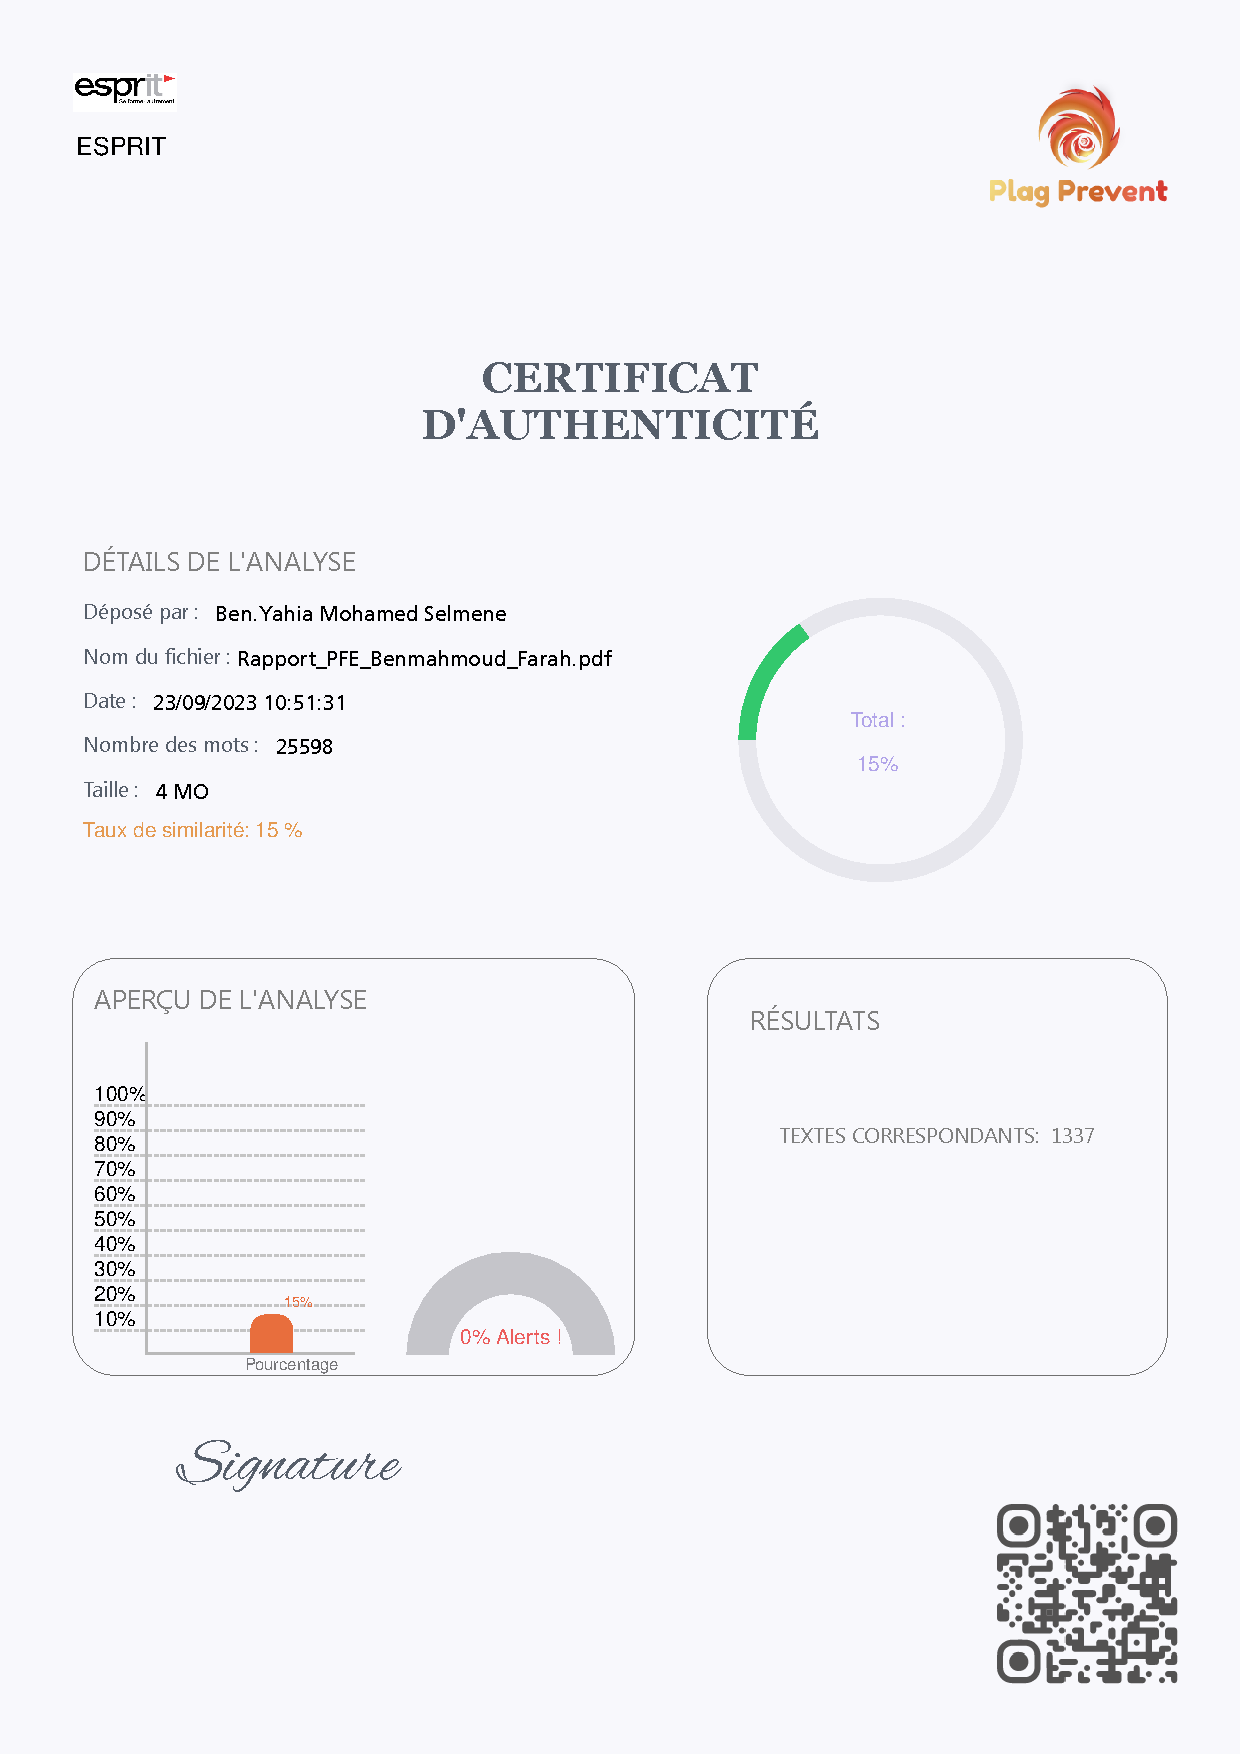
\includepdf{certif.pdf}
% 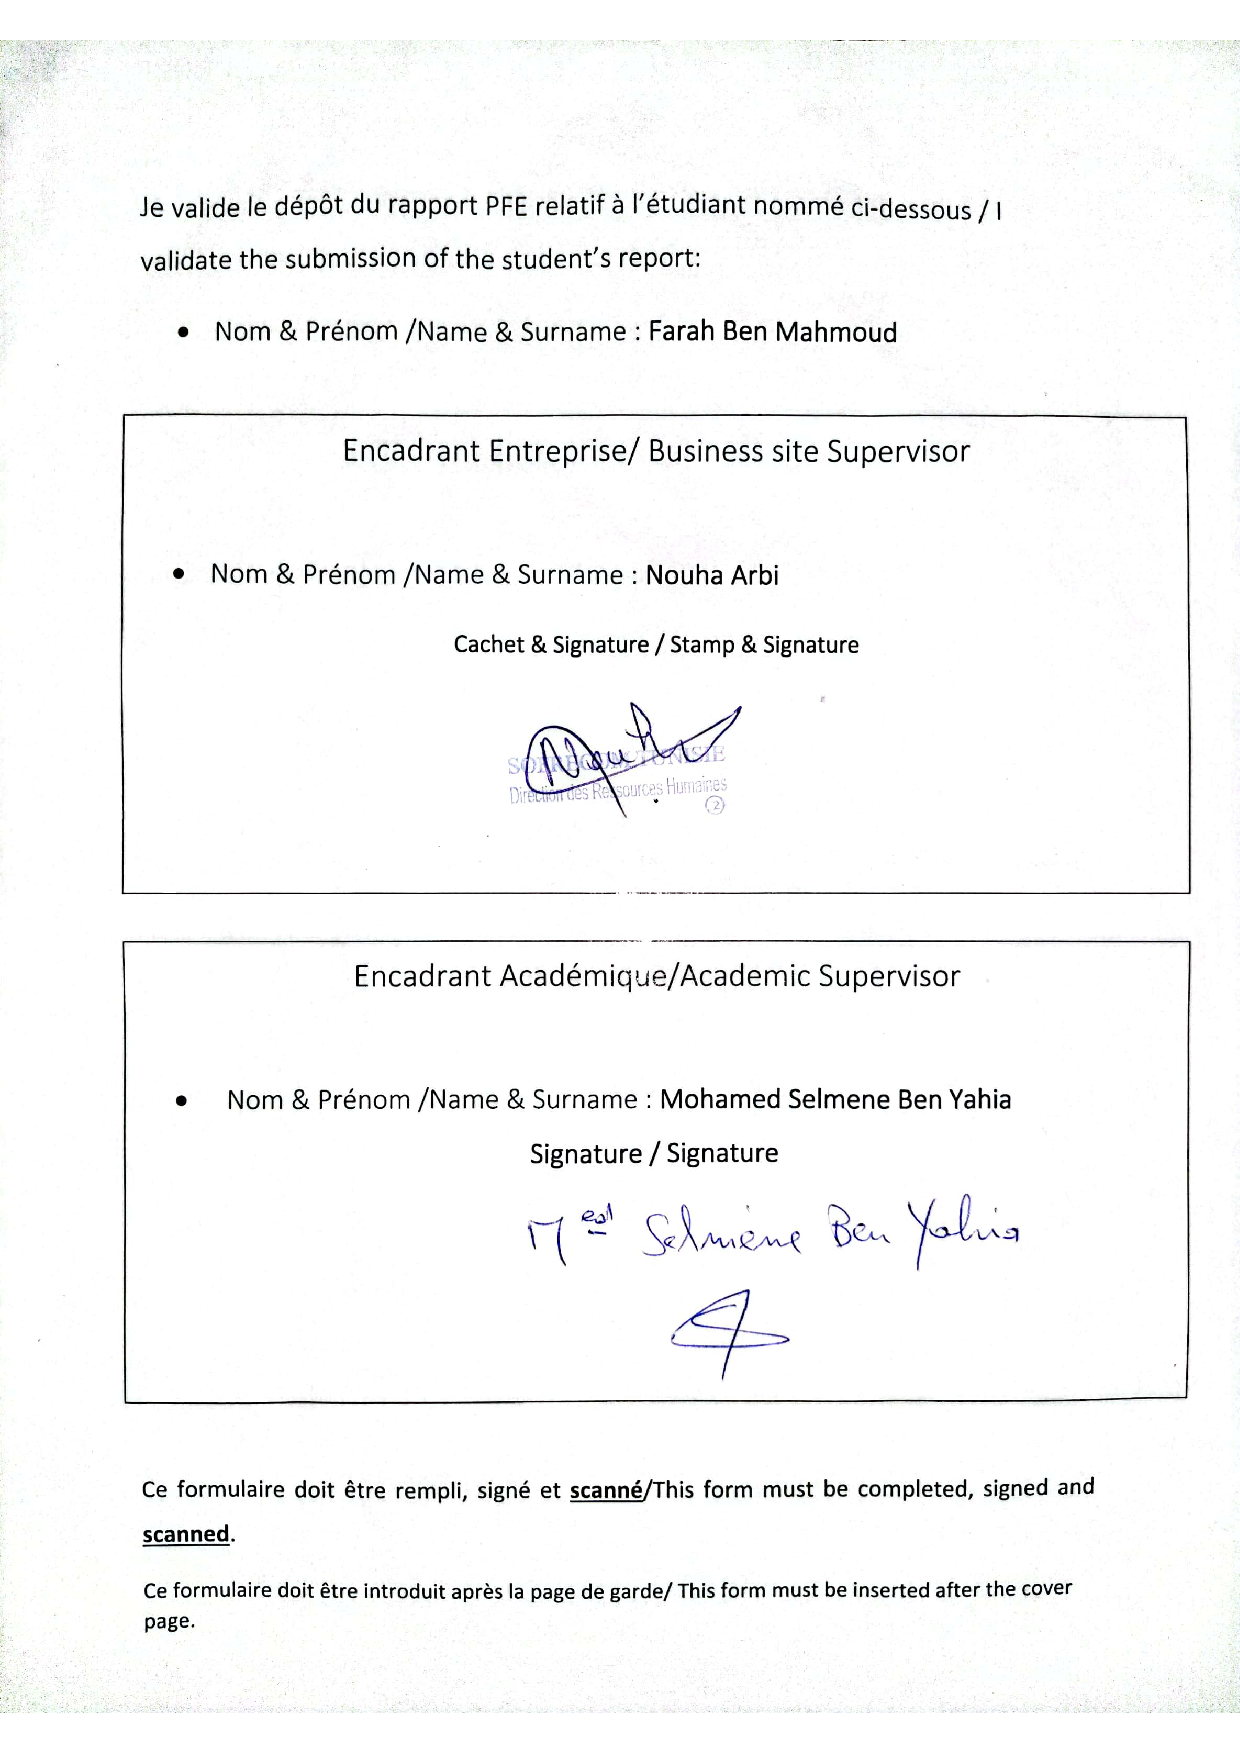
\includepdf{pagegarde.pdf}
\newpage


\addtocontents{toc}{\protect\setcounter{tocdepth}{0}}
    \include{Dedicaces}
    \clearpage
\addtocontents{toc}{\protect\setcounter{tocdepth}{1}} 

\addtocontents{toc}{\protect\setcounter{tocdepth}{0}}
    \chapter*{\huge Remerciements}

\begin{center}
Je tiens à adresser mes plus sincères remerciements à toutes les personnes qui ont contribué, directement ou indirectement, à la réalisation de ce projet. Ces mots de gratitude marquent le début de mon rapport.

\vspace{0.6\baselineskip}
Tout d’abord, je souhaite exprimer ma profonde reconnaissance aux membres du jury pour avoir accepté d’évaluer mon projet de stage de fin d’études.

\vspace{0.6\baselineskip}
Je tiens à adresser mes vifs remerciements à mon encadrant au sein de SIGA, M. Iheb YOUSFI. Son accompagnement, ses conseils avisés et son soutien constant ont été précieux tout au long de ce projet. Sa disponibilité et son expertise m’ont grandement motivé et guidé.

\vspace{0.6\baselineskip}
Mes remerciements vont également à mon encadrante académique, Mme Sahar BEN AZIZA. Ses remarques pertinentes, sa disponibilité et ses orientations ont enrichi mon travail et m’ont permis de progresser.

\vspace{0.6\baselineskip}
Je remercie chaleureusement l’ensemble du corps enseignant de l’École supérieure privée d’ingénierie et de technologie (ESPRIT) pour les bases solides qu’ils m’ont transmises, essentielles à ma première expérience professionnelle.

\vspace{0.6\baselineskip}
Enfin, je tiens à exprimer ma gratitude à l’équipe technique et administrative de SIGA pour leur accueil, leur professionnalisme et l’environnement de travail favorable qu’ils ont su créer, contribuant ainsi au succès de ce projet.

\end{center}
    \clearpage

%Ces 3 listes seront créées automatiquement, en fonction des chapitres et sections du document 
         %lista figuras y tablas no afecta numeración de referencias  
\tableofcontents
\addcontentsline{toc}{chapter}{\listfigurename}
\listoffigures
\addcontentsline{toc}{chapter}{\listtablename}
\listoftables
\addcontentsline{toc}{chapter}{Terminologie}
\chapter*{Terminologie}
%\addcontentsline{toc}{chapter}{Liste des abréviations}
\markboth{Liste des abréviations }{}


\textbf{Automatisation} : c’est lorsque un processus est complètement automatisé et ne requiert aucune intervention d’un utilisateur.
\\

\textbf{Environnement de développement}
: n’est pas seulement un IDE (Integrated
Development Environment) comme Eclipse ou Visual Studio mais les librairies,
les fichiers de configuration et les serveurs en font partie aussi.\\

\textbf{Intégration}
: est la combinaison des parties de code source séparées dont le but
est de déterminer comment elles fonctionnent comme un tout.\\

\textbf{Build}
: présente l’ensemble d’activités dont l’objectif est la construction de l’application. Il comprend plusieurs tâches comme :
\begin{itemize}
    \item La mise à jour du code source depuis le gestionnaire de version
    \item La compilation du code source de l’application
    \item La génération des artefacts\\
\end{itemize}

\textbf{Une tâche (Job)}
: est un ensemble d’instructions que le runner doit exécuter. \cite{ref3}
L’ensemble des jobs est défini dans un fichier YAML. Nous pouvons voir en temps réel le résultat d’une tâche afin que les développeurs puissent savoir si le job a été exécuté avec succès ou bien il a échoué.
Un job peut être automatiquement lancé lorsqu’un commit est poussé ou bien manuellement exécuté. En effet, le job manuel peut être utile, par exemple, pour
automatiser un déploiement, mais ne le déployer que lorsque quelqu’un l’approuve manuellement. En plus, il existe des moyens qui limitent le nombre de personnes
pouvant exécuter un job.\\

\textbf{Artefact (Artifact)}
: est généré par un job en cas d’exécution avec succès. Les
utilisateurs peuvent télécharger cet artefact pour le tester ou bien l’utiliser
directement \cite{ref3}.\\

\textbf{Pipeline}
: est un groupe de jobs exécutés par étapes. En effet, tous les jobs d’une même étape sont exécutés en parallèle s’il y a suffisamment de Runners simultanés disponibles \cite{ref4}.
Le pipeline passe à l’étape suivante lorsque les jobs en cours terminent leur exécution sans erreurs. En cas d’échec d’au moins un job, l'exécution de pipeline s'arrête.\\

\textbf{Runner}
 : est une machine virtuelle, un container Docker ou un cluster de containers. Son rôle principal est de personnaliser l’environnement d’exécution du job \cite{ref4}.
En particulier, GitLab Runner est un projet Open Source utilisé dans la fonctionnalité d’intégration continue GitLab. Ce dernier communique avec le Runner
à travers une API pour exécuter les scripts écrits dans la configuration GitLab-CI.
\\

\textbf{GOROCO}
 : permet de récupérer la valeur exacte de la version \cite{ref5}. Il se décompose en:
 \begin{enumerate}
     \item \textbf{G}eneration: la génération du logiciel
     \item \textbf{R}evision: les services pack (le cas d’un nombre impaire implique que la version a encore des Bugs à éliminer pour la révision suivante)
     \item \textbf{C}orrection: les mises à jour
 \end{enumerate}

 
 
\addcontentsline{toc}{chapter}{Liste des abréviations}
\include{Acronymes}
\addtocontents{toc}{\protect\setcounter{tocdepth}{2}}
 %liste des tables
      %liste des figures
\clearpage
%incluye lo contenido en nomenclatura.tex

\pagenumbering{arabic}
    \addcontentsline{toc}{chapter}{Introduction générale}
    \include{Introduction}
    \clearpage
%incluye lo contenido en introduccion.tex



\chapter{Contexte général}
\section*{Introduction}



Dans ce premier chapitre, nous allons poser les bases de notre travail en explorant son contexte général. Nous débuterons par une présentation de l’organisme d’accueil, la société SIGA, en mettant en lumière son domaine d’expertise et son rôle. Ensuite, nous introduirons le projet en détail, avant d’examiner l’existant afin d’identifier ses limites et les opportunités d’amélioration que notre solution vise à concrétiser. Enfin, nous exposerons la méthodologie suivie pour concevoir ce projet ainsi que les grandes lignes de la solution proposée.



  
% Une section

% Exemple d'une section qui porte une référence à une bibliographie
% NB: il faut bien suivre le syntaxe pour ne pas tomber dans le cas où il y a une référence dans la table des matières.
\section[Organisme d'accueil]{Organisme d'accueil}

\subsection{SIGA}

Créée en 1996, SIGA (Système Informatique et Gestion Automatisée) s’est imposée comme un acteur majeur dans le domaine du développement de logiciels et des solutions informatiques en Tunisie. Basée à Tunis, l’entreprise regroupe une équipe de plus de vingt ingénieurs et six consultants seniors, cumulant entre 5 et 25 ans d’expérience dans la conception et l’intégration de systèmes d’information. Depuis sa fondation, SIGA se distingue par son expertise multidisciplinaire, offrant des services qui couvrent l’ensemble du cycle de vie d’un produit informatique : de l’analyse des besoins à la mise en œuvre, en passant par le développement, la formation et la maintenance.
\begin{figure}[H]
\centering
\includegraphics[scale=0.5]{images/siga.png}
\caption{Logo de SIGA}
\label{fig:Siga_logo}
\end{figure}
    \newpage
\subsection{Secteur d'activité}
SIGA déploie son expertise dans divers secteurs, proposant des solutions technologiques adaptées aux besoins spécifiques de ses clients. Ses principaux domaines d’intervention incluent :
\begin{itemize}
    \item \textbf{Banque et assurance : }développement de systèmes pour optimiser la gestion des processus financiers et administratifs.
    \item \textbf{Industrie : }conception de logiciels pour améliorer la gestion de la production et des ressources.
    \item \textbf{Transports : }mise en place de solutions facilitant la logistique et la coordination opérationnelle.
    \item \textbf{Télécommunications : }création de systèmes pour rationaliser les interactions et la gestion des données.
    \item \textbf{Autres secteurs :}accompagnement à la digitalisation des opérations pour des entreprises variées, avec une présence étendue en Tunisie et dans plusieurs pays africains (Mali, Côte d’Ivoire, Tchad, Mauritanie).
\end{itemize}

\section{Présentation du Projet}
Le projet que j’ai réalisé s’inscrit dans le cadre de mon projet de fin d’études en dernière année à l’École Supérieure Privée d’Ingénierie et de Technologie (ESPRIT). J’ai effectué mon stage au sein de SIGA, une entreprise reconnue pour son expertise dans le développement de logiciels et de solutions informatiques innovantes en Tunisie.

Dans cette section, nous présentons notre projet en détaillant, dans un premier temps, un aperçu du « Portail de Gestion des Approbations avec Workflows Dynamiques et Déploiement Automatisé » et ses spécificités. Dans un second temps, nous aborderons la problématique, l’étude de l’existant, notre contribution ainsi que la méthodologie adoptée pour mener à bien cette mission.
\subsection{Présentation du Portail de Gestion des Approbations}
Le projet « Portail de Gestion des Approbations avec Workflows Dynamiques et Déploiement Automatisé » est une solution conçue pour centraliser et optimiser la gestion des processus d’approbation au sein des organisations. Son objectif principal est de simplifier la soumission, le suivi et la validation des demandes – telles que les congés ou les autorisations – en offrant une interface intuitive et des mécanismes automatisés. Ce portail se distingue par sa capacité à adapter dynamiquement les workflows en fonction des besoins spécifiques de chaque demande, garantissant ainsi une flexibilité et une personnalisation optimales.\\
\\
    \newpage
Le portail prend en charge divers types de demandes et génère des outputs variés, notamment des notifications par email ou push notification, des statuts en temps réel, et des rapports analytiques sous forme de tableaux de bord. À terme, il vise à gérer un volume significatif de requêtes quotidiennes tout en assurant une traçabilité complète des actions effectuées. Développé avec Angular pour le frontend, Spring Boot pour le backend, et Camunda pour l’orchestration des workflows, le système repose sur une architecture moderne déployée via Docker et orchestrée par Kubernetes. Il est hébergé sur plusieurs environnements distincts : développement (DEV), tests (TEST) et production (PROD), avec une infrastructure évolutive adaptée à chaque contexte.\\
\\
Chez SIGA, ce projet joue un rôle clé dans la digitalisation des processus internes, et toute interruption pourrait affecter la fluidité des opérations, rendant sa disponibilité une priorité essentielle.

\subsection{Spécificités du Portail de Gestion des Approbations}
Le portail est un outil de gestion des processus qui permet aux utilisateurs de soumettre et de suivre des demandes via différents canaux et fonctionnalités, notamment : \begin{itemize}
    \item \textbf{Workflows dynamiques: }des processus personnalisables définis avec Camunda.
    \item \textbf{Suivi en temps réel: }un statut actualisé et un historique des actions.
    \item \textbf{Reporting: }des tableaux de bord pour analyser les processus.
    \item \textbf{Notifications: }des alertes automatiques par email ou temps réel.
\end{itemize}
\subsection{ Problématique } 
Dans de nombreuses organisations, les processus d’approbation sont encore réalisés de manière manuelle. Cela engendre plusieurs problématiques :
\begin{itemize}
  \item \textbf{Lenteur des traitements: }Les délais sont souvent rallongés à cause des allers-retours entre les différents acteurs.
  \item \textbf{Manque de traçabilité :} Il est difficile de connaître l’état d’avancement d’une demande ou de retracer les actions passées.
  \item \textbf{Risque d’erreurs humaines : }En raison du manque d’automatisation, certaines étapes peuvent être oubliées ou mal exécutées.
\end{itemize}

\subsection{ Situation actuelle et Critiques } 
Actuellement, pour obtenir une approbation (congé, autorisation...), le processus suit généralement les étapes suivantes :
\begin{enumerate}
    \item Remplissage manuel d’un formulaire papier ou d’un document bureautique (Word, Excel).
    \item Transmission physique ou par email au supérieur hiérarchique.
    \item Approbation manuelle, parfois verbale, sans traçabilité.
    \item Notification au demandeur uniquement si ce dernier relance.
\end{enumerate}
\subsubsection*{Inconvénients:}
\begin{itemize}
    \item \textbf{Non-centralisation} : Les demandes sont éparpillées (emails, papiers, discussions).
    \item \textbf{Perte de temps} : Les relances sont fréquentes.
    \item \textbf{Absence de supervision globale} : Aucune visibilité d’ensemble pour l’administration.
    \item \textbf{Aucune possibilité d’analyse} : Pas de données statistiques sur les demandes, les délais, les refus, etc.
\end{itemize}

\section{Solution proposée}

Afin de répondre aux limites identifiées dans le processus actuel, il est proposé de mettre en place un \textbf{Portail Web de Gestion des Approbations} moderne, centralisé et automatisé. Ce portail repose sur une architecture modulaire et des technologies éprouvées pour assurer une solution performante, évolutive et facilement maintenable.

\subsection*{Automatisation des workflows avec Camunda BPM}

Le cœur de la solution repose sur l'intégration de \textbf{Camunda BPM}, un moteur de workflow open-source basé sur le standard BPMN (Business Process Model and Notation). Chaque type de demande (congé, achat, autorisation, etc.) est modélisé sous forme de processus graphique. Ces workflows définissent les différentes étapes à suivre, les rôles impliqués et les règles de validation.

L’utilisation de Camunda permet :
\begin{itemize}
    \item La \textbf{définition claire et visuelle} des processus métiers.
    \item L’\textbf{exécution automatique} des étapes selon les règles définies.
    \item La \textbf{flexibilité} de modifier les processus sans redéployer l’application.
    \item L’\textbf{assignation dynamique} des tâches aux utilisateurs concernés.
\end{itemize}

\subsection*{Digitalisation de la soumission des demandes}

L’interface utilisateur, développée avec \textbf{Angular}, permet aux utilisateurs de soumettre leurs demandes via des formulaires en ligne ergonomiques et adaptés au type de demande. Chaque formulaire est connecté à une instance de processus Camunda qui orchestre automatiquement les étapes suivantes. Cette digitalisation permet de :
\begin{itemize}
    \item Réduire les erreurs de saisie grâce à des contrôles intégrés.
    \item Gagner du temps en supprimant les supports papier.
    \item Standardiser la soumission et le traitement des demandes.
\end{itemize}
\newpage
\subsection*{Suivi en temps réel et notifications automatiques}

Chaque utilisateur peut suivre en temps réel le statut de ses demandes (approuvée, rejetée ou en cours de traitement). Le portail intègre un système de \textbf{notifications en temps réel} directement dans l’interface de l’application, basé sur des technologies de type WebSocket:

\begin{itemize}
    \item Alerte à l'approbateur lorsqu’une tâche lui est assignée.
    \item Notification au demandeur une fois la décision prise.
    \item Rappels pour les tâches non traitées dans un délai défini.
\end{itemize}

Ce mécanisme renforce la réactivité des acteurs et limite les retards.

\subsection*{Infrastructure moderne, scalable et résiliente}

L’ensemble de l’application est conteneurisé à l’aide de \textbf{Docker} afin de garantir une portabilité maximale et un déploiement simplifié. Le déploiement se fait sur un cluster \textbf{Kubernetes} pour bénéficier :
\begin{itemize}
    \item D’une haute disponibilité des services.
    \item D’un équilibrage de charge automatique.
    \item D’une scalabilité horizontale en fonction de la charge.
\end{itemize}

\subsection*{Pipeline DevOps pour l’intégration et le déploiement continus}

Un pipeline CI/CD est mis en place avec \textbf{ArgoCD} pour automatiser :
\begin{itemize}
    \item La compilation et les tests des composants backend et frontend.
    \item La construction des images Docker.
    \item Le déploiement automatique sur l’environnement de production.
\end{itemize}

Cela permet de garantir la rapidité, la fiabilité et la répétabilité du processus de livraison.

\subsection*{Analyse des performances et tableaux de bord}

Des tableaux de bord sont mis à disposition des administrateurs pour visualiser :
\begin{itemize}
    \item Le nombre de demandes traitées par type ou par service.
    \item Les délais moyens de traitement.
    \item Les goulets d’étranglement dans les workflows.
\end{itemize}

Ces indicateurs permettent d’optimiser les processus métier et de prendre des décisions basées sur des données concrètes.


\newpage
\section{Méthodologie de gestion de projet}
\normalsize{

Afin d'assurer le bon déroulement de notre projet, tout en respectant les contraintes de qualité, de délais et les attentes fonctionnelles, il est essentiel d’adopter une méthodologie adaptée qui structure et optimise les différentes phases de travail.
\subsection{Méthodologies agiles}
Les méthodologies agiles représentent une nouvelle génération d’approches de gestion de projet, axées sur des cycles itératifs, adaptatifs et incrémentaux. Elles permettent une réévaluation régulière des besoins, facilitent l’évolution des exigences et garantissent une livraison progressive et maîtrisée des fonctionnalités. \cite{ref10}.\\ 
Ces méthodes reposent sur des principes forts, tels que :
\begin{itemize}
    \item L’acceptation du changement tout au long du cycle de développement.
    \item La collaboration constante avec le client, considéré comme partie prenante active.
    \item L’accent mis sur la valeur fonctionnelle livrée à chaque itération.
    \item La priorité donnée aux interactions humaines plutôt qu’aux processus rigides.
\end{itemize}
Les méthodes agiles favorisent ainsi la réactivité, l’amélioration continue et l’adaptabilité face à un environnement en perpétuelle évolution.
\subsection{Méthode Scrum }
Parmi les différentes approches agiles, la méthodologie Scrum s’est imposée comme une référence incontournable. Elle fournit un cadre structuré mais souple permettant d’organiser efficacement le travail d’équipe, tout en maximisant la productivité et la qualité du produit livré.\\
\\
Nous avons opté pour Scrum, car cette méthodologie répond parfaitement aux besoins des projets complexes en nous offrant une flexibilité optimale et une forte capacité d’adaptation face aux imprévus.\\
\\
Le contexte méthodologique de Scrum s'articule, tel que le montre la figure  \ref{scrumSpirale}, autour de la définition des fonctions, d'un tempo bien rythmé, d'éléments concrets et des réunions particulières.
 

\begin{figure}[H]
\centering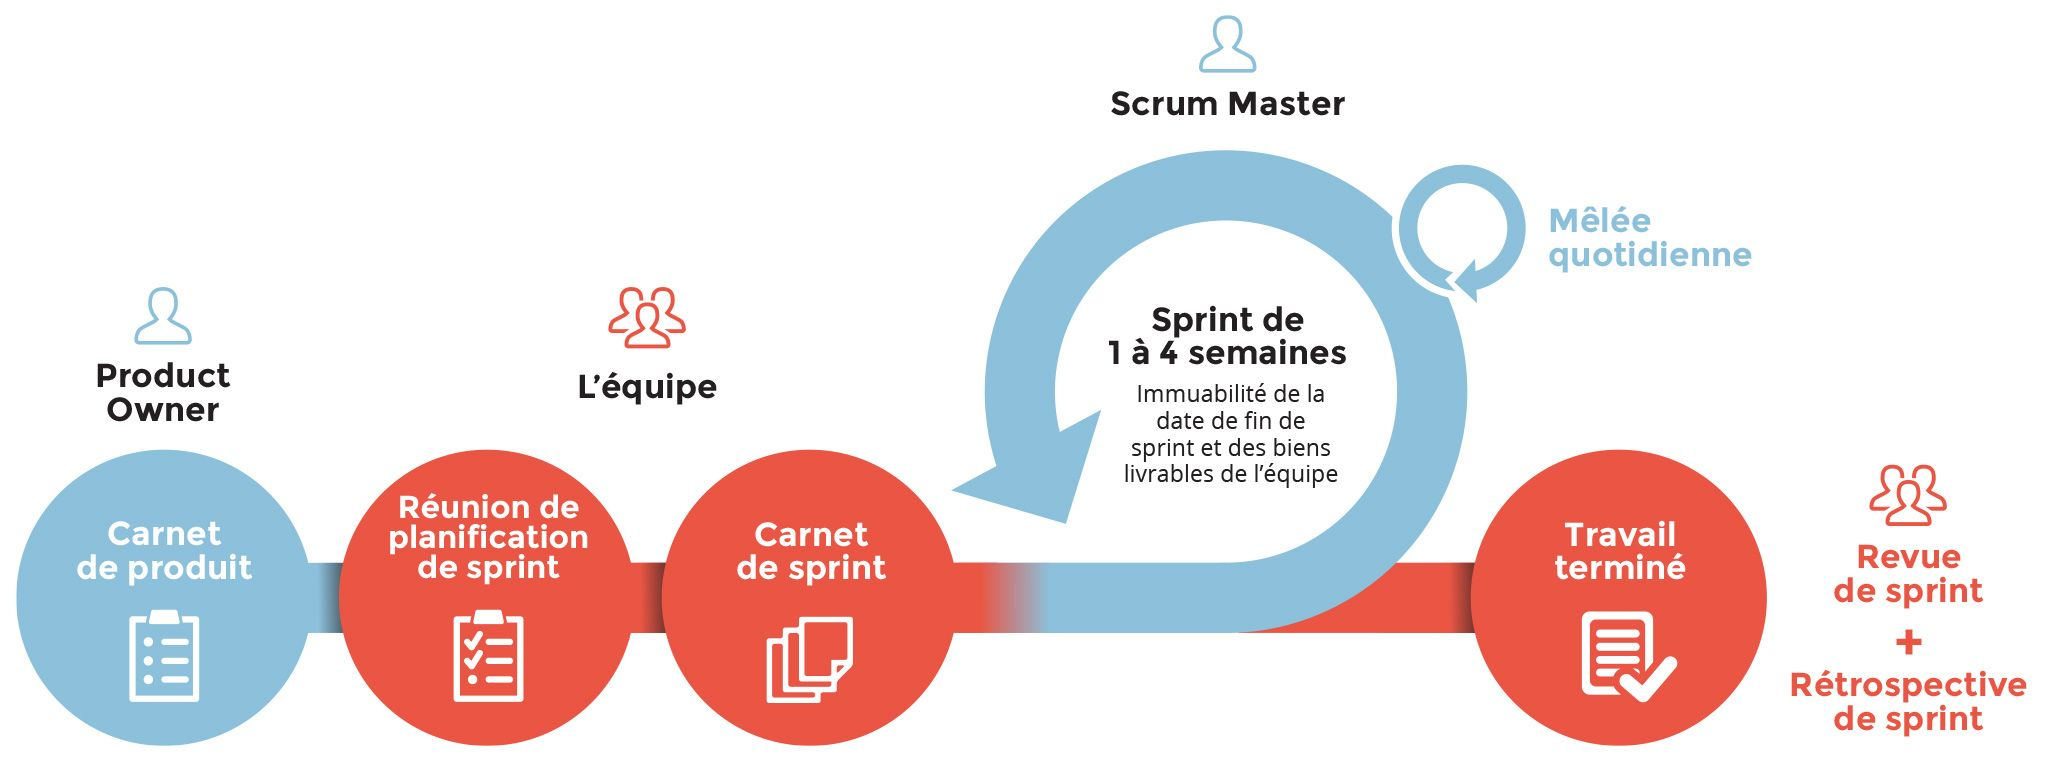
\includegraphics[scale=0.21]{images/scrum.jpeg}
\caption{Le cycle de vie en Scrum}
\label{scrumSpirale}
\end{figure}


\noindent \bfseries Les Rôles \mdseries : \\
Scrum définit trois rôles clés, indispensables à la réussite du projet :
\begin{itemize}
\item \noindent \bfseries Le Product Owner  \mdseries : Il est fréquent qu'un spécialiste de domaine assume le rôle de représentant officiel du client au sein d'un projet Scrum. Son rôle principal consiste à définir les besoins fonctionnels, établit les priorités dans le Product Backlog et veille à la satisfaction du client.\newline

\item \noindent \bfseries Le Scrum Master \mdseries : Garant de la méthode Scrum, il facilite le travail de l’équipe en supprimant les obstacles et en s’assurant que les pratiques agiles sont correctement appliquées.\\

\item \noindent \bfseries L’Équipe \mdseries : Les membres responsable de la conception, du développement, des tests et de la livraison des fonctionnalités à la fin de chaque sprint. Ils sont auto-organisés et multidisciplinaires. 
\end{itemize}

\noindent \bfseries Le Rythme Itératif \mdseries : 
\begin{itemize}
\item \noindent \bfseries Sprint  \mdseries : Le travail est organisé en cycles courts appelés sprints, d’une durée généralement comprise entre 2 et 4 semaines. À chaque sprint, une version incrémentale du produit est développée, testée et potentiellement livrable.

\end{itemize}

\noindent \bfseries Les Artefacts \mdseries : 
\begin{itemize}
\item \noindent \bfseries Product Backlog  \mdseries :  Liste hiérarchisée de toutes les fonctionnalités à développer, rédigées sous forme de User Stories. Ce backlog est régulièrement mis à jour en fonction des retours du client.

\item \noindent \bfseries Sprint Backlog  \mdseries : Sous-ensemble du Product Backlog sélectionné pour être réalisé lors d’un sprint donné. Il contient les User Stories détaillées et les tâches associées.
\end{itemize}
\newpage
\noindent \bfseries les Evénements \mdseries : 
\begin{itemize}
\item \noindent \bfseries Sprint Planning  \mdseries : Réunion de planification marquant le début de chaque sprint. L’équipe sélectionne les éléments à développer et définit les objectifs à atteindre.
\item \noindent \bfseries Daily Scrum (Mêlée quotidienne)  \mdseries : Courte réunion quotidienne, souvent appelée "stand-up" en raison de sa brièveté (15 minutes maximum), visant à synchroniser les efforts de l’équipe. Chaque membre partage trois points : ce qu’il a accompli depuis la dernière mêlée, ce qu’il prévoit de faire avant la prochaine, et les éventuels blocages rencontrés. Facilitée par le Scrum Master, cette rencontre n’est pas destinée à résoudre les problèmes sur-le-champ, mais à les identifier pour un traitement ultérieur. Elle favorise la transparence, renforce la collaboration et permet d’ajuster rapidement le plan du sprint si nécessaire.
\item \noindent \bfseries Definition of Done (DoD) \mdseries :
Ensemble de critères définissant qu’une tâche est considérée comme terminée (tests réussis, documentation rédigée, code relu, etc.).
\item \noindent \bfseries Definition of Ready (DoR) \mdseries :
Ce concept repose sur une compréhension commune des préparatifs requis pour une tâche, intégrant une liste de contrôle pour établir les User Stories. Pour être considérées comme prêtes à être mises en œuvre, les User Stories doivent répondre à plusieurs exigences, notamment la description exhaustive des scénarios d'utilisation, la disponibilité des ressources essentielles, des critères d'acceptation clairement définis et vérifiables, une taille adaptée, une présentation à l'équipe par le propriétaire du produit, des méthodes de test fonctionnelles, une estimation fiable de leur taille relative basée sur l'expérience utilisateur, ainsi que la spécification des appareils ciblés.

\item \noindent \bfseries Revue de Sprint  \mdseries : Réunion organisée à la fin de chaque sprint pour évaluer le travail accompli. L’équipe présente l’incrément terminé au Product Owner et aux parties prenantes, qui valident sa conformité aux attentes. Si nécessaire, des ajustements sont apportés au "Product Backlog" pour refléter l’évolution des besoins ou des priorités. D’une durée maximale de 4 heures pour un sprint d’un mois, cette étape vise à garantir que le projet progresse efficacement, tout en maintenant un alignement constant avec les objectifs stratégiques et les exigences changeantes.

\item \noindent \bfseries Rétrospective de Sprint  \mdseries : 
Rencontre tenue immédiatement après la revue, dédiée à l’amélioration continue. L’équipe, guidée par le Scrum Master, analyse le sprint écoulé en identifiant ce qui a bien fonctionné, les difficultés rencontrées, et les opportunités d’optimisation. Des actions concrètes sont définies pour le sprint suivant, comme ajuster les processus ou résoudre des blocages récurrents. Limitée à 3 heures pour un sprint d’un mois, cette réunion renforce l’auto-organisation de l’équipe et assure une progression constante dans la qualité et l’efficacité du travail.

\end{itemize}
\newpage
\section{Langage de modélisation : UML}
Le langage UML (Unified Modeling Language) est un langage standardisé de modélisation utilisé dans la conception orientée objet des systèmes logiciels. Il permet de représenter, visualiser, spécifier, construire et documenter de manière formelle les différents aspects d’un système, tant structurels que comportementaux.\\
\\
UML repose sur un ensemble de diagrammes graphiques permettant de décrire les éléments clés d’un système : les classes, les objets, les interactions, les activités, les cas d'utilisation, etc. Ces représentations facilitent la communication entre les différents acteurs du projet (développeurs, analystes, chefs de projet) et garantissent une compréhension commune du fonctionnement global du système.\\
\\
Dans le cadre de notre projet, nous avons choisi d’utiliser UML pour modéliser les différentes composantes de notre application. Ce choix s’explique par la richesse expressive d’UML, sa capacité à structurer efficacement un système complexe, et sa large adoption dans l’industrie comme outil de conception et de documentation. La figure \ref{umlLogo} présente le logo du language de modélisation UML.\\

\begin{figure}[H]
\centering
\includegraphics[scale=0.5]{images/UML_logo.png}
\caption{Interface de ClickUp}
\label{umlLogo}
\end{figure}
\section{Outils adoptés pour la gestion de projet}
\normalsize{
Pour assurer le succès de notre projet et garantir une livraison réussie de notre produit, nous avons mis en place un ensemble d'outils de gestion de projet stratégiques, parmi lesquels nous pouvons citer :
\begin{itemize}
    \item \noindent \bfseries Git \mdseries : Un système de contrôle de version permettant de suivre les modifications apportées aux fichiers de code, facilitant ainsi une collaboration fluide et efficace entre plusieurs contributeurs.
    \item \noindent \bfseries GitLab \mdseries : Une plateforme de gestion de dépôts basée sur Git, qui simplifie le suivi et l’organisation de nos ressources tout en optimisant leur gestion.
    \item \noindent \bfseries Microsoft Teams \mdseries : Un outil collaboratif de communication qui renforce les interactions au sein de l’équipe, favorisant une coordination transparente et une communication améliorée.
    \newpage
    \item \noindent \bfseries ClickUp \mdseries : Une solution open source de gestion de projet, essentielle pour planifier, suivre et gérer les tâches, contribuant ainsi à une administration efficace et structurée de l’ensemble du projet. La figure \ref{clickup} présente l'interface de ClickUp.
\end{itemize}

\begin{figure}[H]
\centering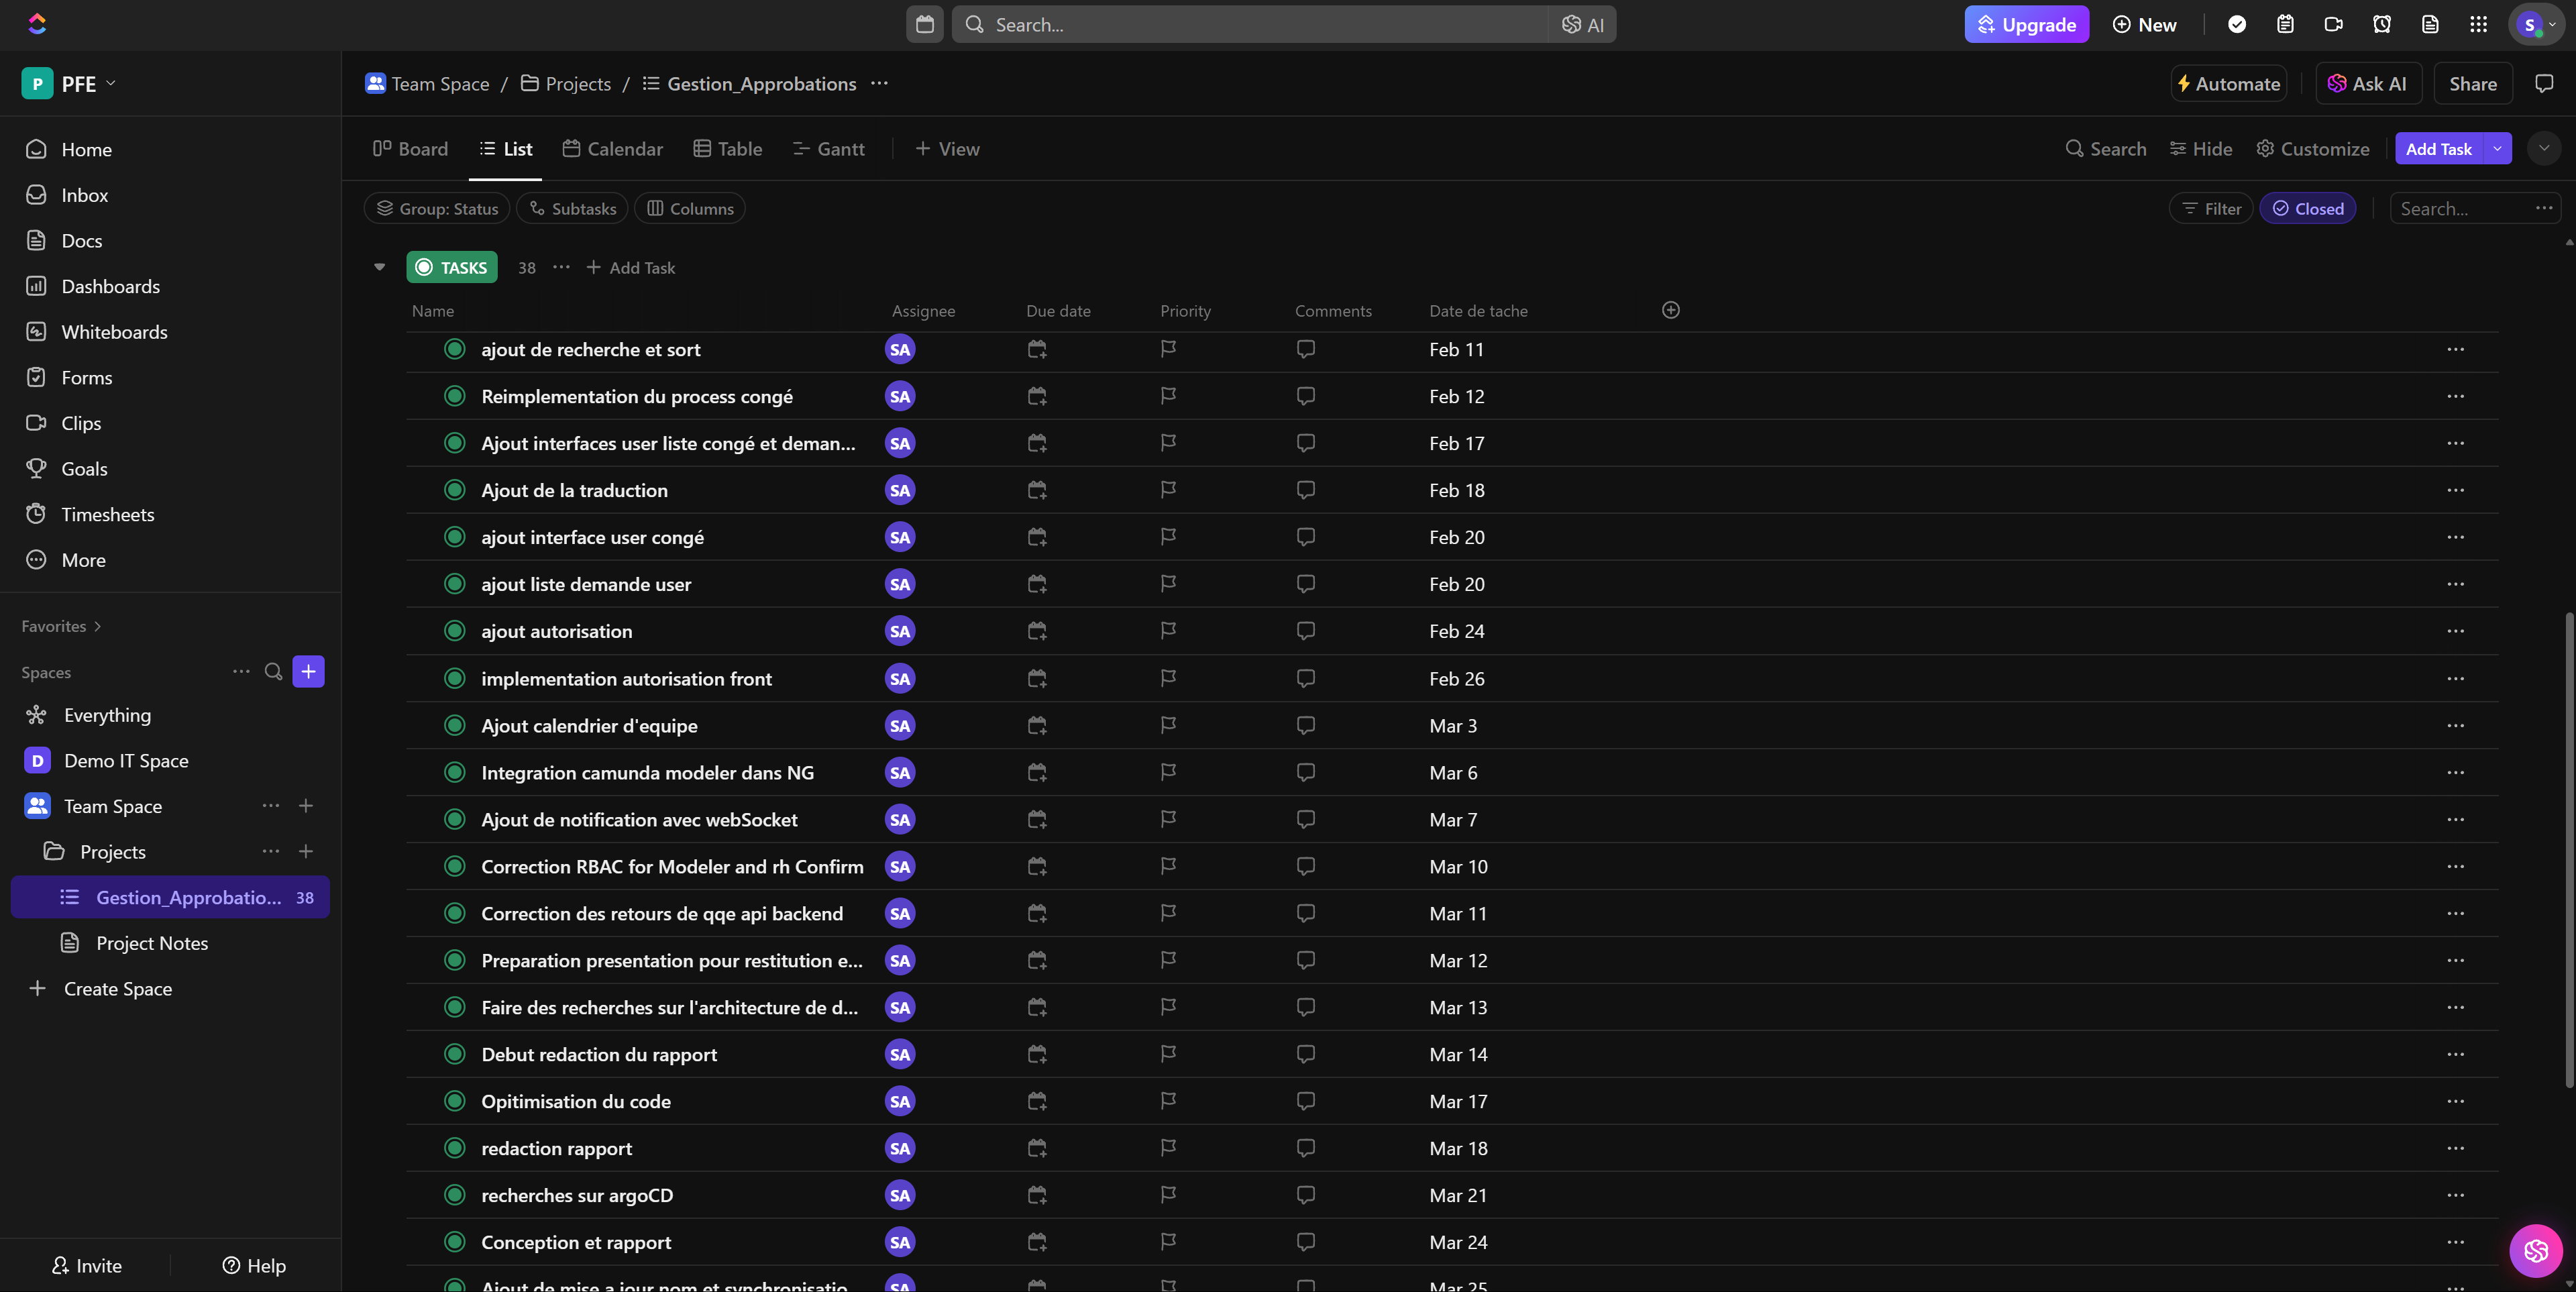
\includegraphics[scale=0.32]{images/clickUp.png}
\caption{Interface de ClickUp}
\label{clickup}
\end{figure}

\section*{Conclusion}

\normalsize{

Dans ce premier chapitre, nous avons introduit l’organisme d’accueil tout en offrant un aperçu général de la problématique et des objectifs du projet. \\
Nous avons également décrit la méthodologie retenue ainsi que le formalisme encadrant le processus mis en œuvre pour le développement de notre application. \\
Le chapitre suivant se concentrera sur l’analyse de la solution existante, en mettant en lumière ses limites et en proposant une nouvelle solution à concevoir.

}

}
}

\clearpage

\chapter{Sprint 0 : Analyse et Spécification des besoins}
\section{Introduction}
Ce chapitre est consacré à l’analyse des besoins pour le développement du Portail de Gestion des Approbations. Nous y identifions les exigences fonctionnelles et non fonctionnelles du système, puis nous illustrons la modélisation à l’aide de diagrammes UML tels que les cas d’utilisation et le diagramme de classes.\\
Nous présentons ensuite le Backlog produit défini selon la méthodologie Scrum, avant de conclure par une présentation des principaux outils utilisés dans cette phase.
\section{Capture des besoins}
Dans cette section nous présentons les acteurs du système,les besoins fonctionnels et non
fonctionnels présents dans le projet.
\subsection{Identification des acteurs}
Notre système contient quatre acteurs ,illustrés dans la figure \ref{tab:actors}, qui sont :
\begin{itemize}
    \item \textbf{Administrateur} : Gère l’ensemble du système, incluant les utilisateurs et les configurations globales (e.g., permissions, intégrations).
    \item \textbf{Manager} : Soumet, consulte et traite les demandes (validation/rejet) des employés qu’il supervise.
    \item \textbf{RH (Ressources Humaines)} : Gère les congés, soumet, consulte et traite les demandes, tout en assurant le suivi des politiques RH.
    \item \textbf{Utilisateur} : Employé qui soumet des demandes (congés, absences) et consulte ses propres demandes et soldes de congés.
\end{itemize}
\begin{figure}[h]
\vspace*{-2cm}
    \centering
    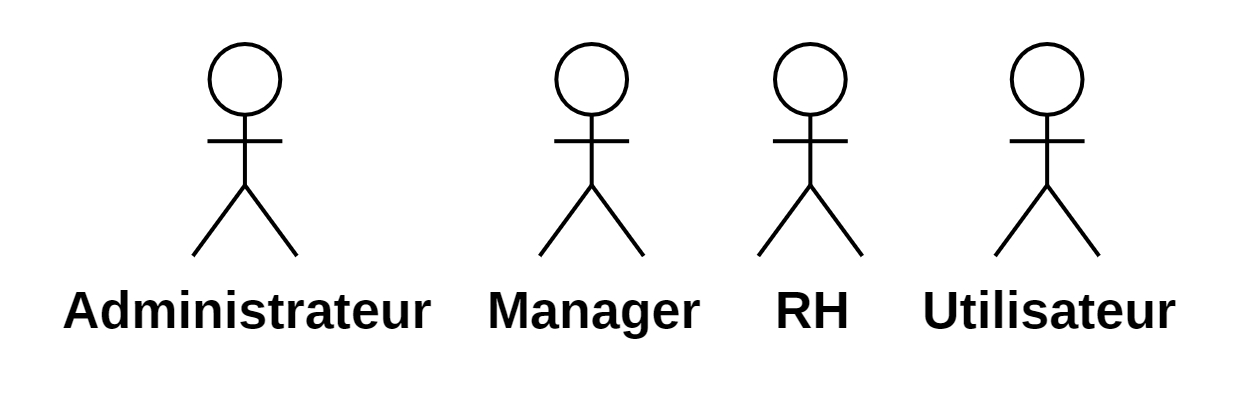
\includegraphics[width=6cm]{images/actors.jpg} 
    \caption{Les acteurs}
    \label{tab:actors}
\end{figure}
 \subsection{Identification des besoins fonctionnels}
Les besoins fonctionnels sont les interactions entre l'acteur(Une personne,un matériel ou un logiciel) et le système de manière à exploiter les fonctionnalités de ce dernier.
Notre système offre aux acteurs la possibilité de faire certaines tâches. \\
\vspace*{-0.5cm}
\begin{table}[!ht]
Le tableau \ref{tab:actors} illustre le rôle de chaque acteur dans ce système.
\begin{center}
\vspace*{-0.5cm}
\caption{tab:Les rôles des acteurs}
\begin{tabular}{ | m{4cm} | m{9cm}| } 
\hline
Administrateur &
- S'authentifier. \vskip0.05cm
- Se déconnecter. \vskip0.05cm
- Gérer les utilisateurs.\vskip0.05cm
- Consulter les processus métiers. \vskip0.05cm
- Consulter les demandes d'approbations.
 \\ 
\hline
Utilisateur &
- S’authentifier.\vskip0.05cm
- Se déconnecter.\vskip0.05cm
- Consulter ses demandes.\vskip0.05cm
- Consulter ses congés.\vskip0.05cm
- Soumettre une demande.\vskip0.05cm
- Recevoir une notifications.\vskip0.05cm
- Consulter les rapports.\vskip0.05cm
- Gérer son profil.\vskip0.05cm
- Consulter le calendrier d'équipe.\vskip0.05cm
- Consulter les membres d'équipe.\vskip0.05cm
- Consulter ses crédits.
\\
\hline
Manager / RH &
- S’authentifier.\vskip0.05cm
- Se déconnecter.\vskip0.05cm
- Consulter ses demandes.\vskip0.05cm
- Consulter ses congés.\vskip0.05cm
- Soumettre une demande.\vskip0.05cm
- Recevoir une notifications.\vskip0.05cm
- Consulter les rapports.\vskip0.05cm
- Gérer son profil.\vskip0.05cm
- Consulter le calendrier d'équipe.\vskip0.05cm
- Consulter les membres d'équipe.\vskip0.05cm
- Consulter ses crédits.\vskip0.05cm
- Consulter ses taches accomplies. \vskip0.05cm
- Traiter une Demande.
\\
\hline
\end{tabular}
\label{1}
\end{center}
\end{table}
\newpage
\subsection{Identification des cas d'utilisation}
\begin{itemize}
 \item \textbf{S'authentifier:} L'authentification est le cas d'utilisation qui permet à tous les utilisateurs (Administrateur, Utilisateur, Manager, RH) d'accéder à la plateforme. Il contient deux champs à remplir, qui sont le nom d'utilisateur et le mot de passe, et un bouton de validation pour accéder aux fonctionnalités de la plateforme en cas de succès de l'authentification.
 
 \item \textbf{Se déconnecter:} Les utilisateurs (Administrateur, Utilisateur, Manager, RH) peuvent se déconnecter du système en cliquant sur le bouton "Déconnexion". Le système vérifie l'existence et la conformité des coordonnées de l'utilisateur avant de le quitter.

 \item \textbf{Gérer les utilisateurs:} À travers ce cas d'utilisation, l'Administrateur est le seul à avoir le droit de gérer les utilisateurs de la plateforme, en incluant l'ajout, la consultation, la modification et la suppression des utilisateurs

 \item \textbf{Consulter les processus métiers:} L'Administrateur a la possibilité de consulter les différents processus métiers définis dans le système pour mieux comprendre les opérations internes et leur suivi.

 \item \textbf{Consulter les demandes d'approbation:} L'Administrateur peut accéder aux demandes d'approbation soumises pour les consulter.

 \item \textbf{Consulter ses demandes:} Les Utilisateurs, les Managers et les RH peuvent consulter l'historique de leurs demandes dans la plateforme.

 \item \textbf{Consulter ses congés:} Les utilisateurs, les Managers et les RH peuvent consulter la liste de leurs congés, passés et à venir, ainsi que leur solde restant.

 \item \textbf{Soumettre une demande:} Les Utilisateurs, les Managers et les RH peuvent soumettre une nouvelle demande via la plateforme. Cette demande peut concerner des congés, des absences ou d'autres requêtes spécifiques.

 \item \textbf{Recevoir une notification:} Ce cas permet aux Utilisateurs, Managers et aux RH de recevoir des notifications concernant les actions importantes, comme la validation d’une demande, ou des rappels de tâches.

 \item \textbf{Consulter les rapports:} Les Utilisateurs, les Managers et les RH peuvent consulter les rapports concernant leurs activités, comme les demandes soumises, les congés, les tâches accomplies, etc.

 \item \textbf{Gérer son profil:} Ce cas permet à chaque acteur (Utilisateur, Manager, RH) de gérer son profil personnel en modifiant ses informations comme son mot de passe, son adresse e-mail, etc.

 \item \textbf{Consulter le calendrier d'équipe:} Ce cas permet à l'Utilisateur, au Manager et au RH de consulter le calendrier de leur équipe, afin de voir les absences, les congés et les événements à venir.
\newpage
 \item \textbf{Consulter les membres de l'équipe:} Les Utilisateurs, les Managers et les RH peuvent consulter la liste des membres de leur équipe, leurs informations et les tâches qui leur sont attribuées.\\

 \item \textbf{Consulter ses crédits:} Ce cas permet aux Utilisateurs, aux Managers et aux RH de consulter le solde de leurs crédits de congé ou autres types de crédits sur la plateforme.

 \item \textbf{Consulter ses tâches accomplies:} Les Managers et les RH peuvent consulter les tâches accomplies par ses subordonnés, pour le suivi des activités et des performances.

 \item \textbf{Traiter une demande:} Le Manager  et l'RH sont en charge de traiter les demandes soumises, en les validant ou en les rejetant, selon les critères définis dans la plateforme.
\end{itemize}
\subsection{Identification des besoins non fonctionnels}

Les besoins non fonctionnels décrivent les contraintes et les exigences de qualité que doit respecter le système. Ils garantissent la performance, la fiabilité et la sécurité de l'application. Voici les principaux besoins non fonctionnels identifiés pour notre projet :

\begin{itemize}
    \item \textbf{Performance :} Le système doit offrir une bonne réactivité, avec un temps de réponse inférieur à 2 secondes pour l'affichage des principales fonctionnalités. Il doit également supporter un nombre élevé de connexions simultanées sans dégradation notable des performances.
    
    \item \textbf{Sécurité :} Le système doit garantir la confidentialité, l’intégrité et la disponibilité des données. L’authentification des utilisateurs doit être sécurisée, et les accès doivent être strictement contrôlés selon le rôle de chaque utilisateur.
    
    \item \textbf{Fiabilité :} Le système doit être capable de fonctionner de manière continue sans erreurs critiques, avec un taux de disponibilité supérieur à 99.5\%.

    \item \textbf{Scalabilité :} Le système doit pouvoir évoluer facilement pour prendre en charge un plus grand nombre d’utilisateurs ou de données sans refonte majeure de l’architecture.
    
    \item \textbf{Traçabilité :} Le système doit enregistrer les actions importantes effectuées par les utilisateurs (audit logs) pour permettre un suivi en cas d’incident ou d’investigation.
\end{itemize}
\newpage
\section{Diagramme de cas d'utilisation globale}
Le diagramme de cas d'utilisation globale illustré dans la figure \ref{usecaseDiagram} consiste à décrire les fonctions fondamentales et identifie , également la relation et les interactions entre le système et ses acteurs.
\begin{figure}[H]
\begin{adjustwidth}{-2.7cm}{-2cm} % reduce left and right margins locally
\centering
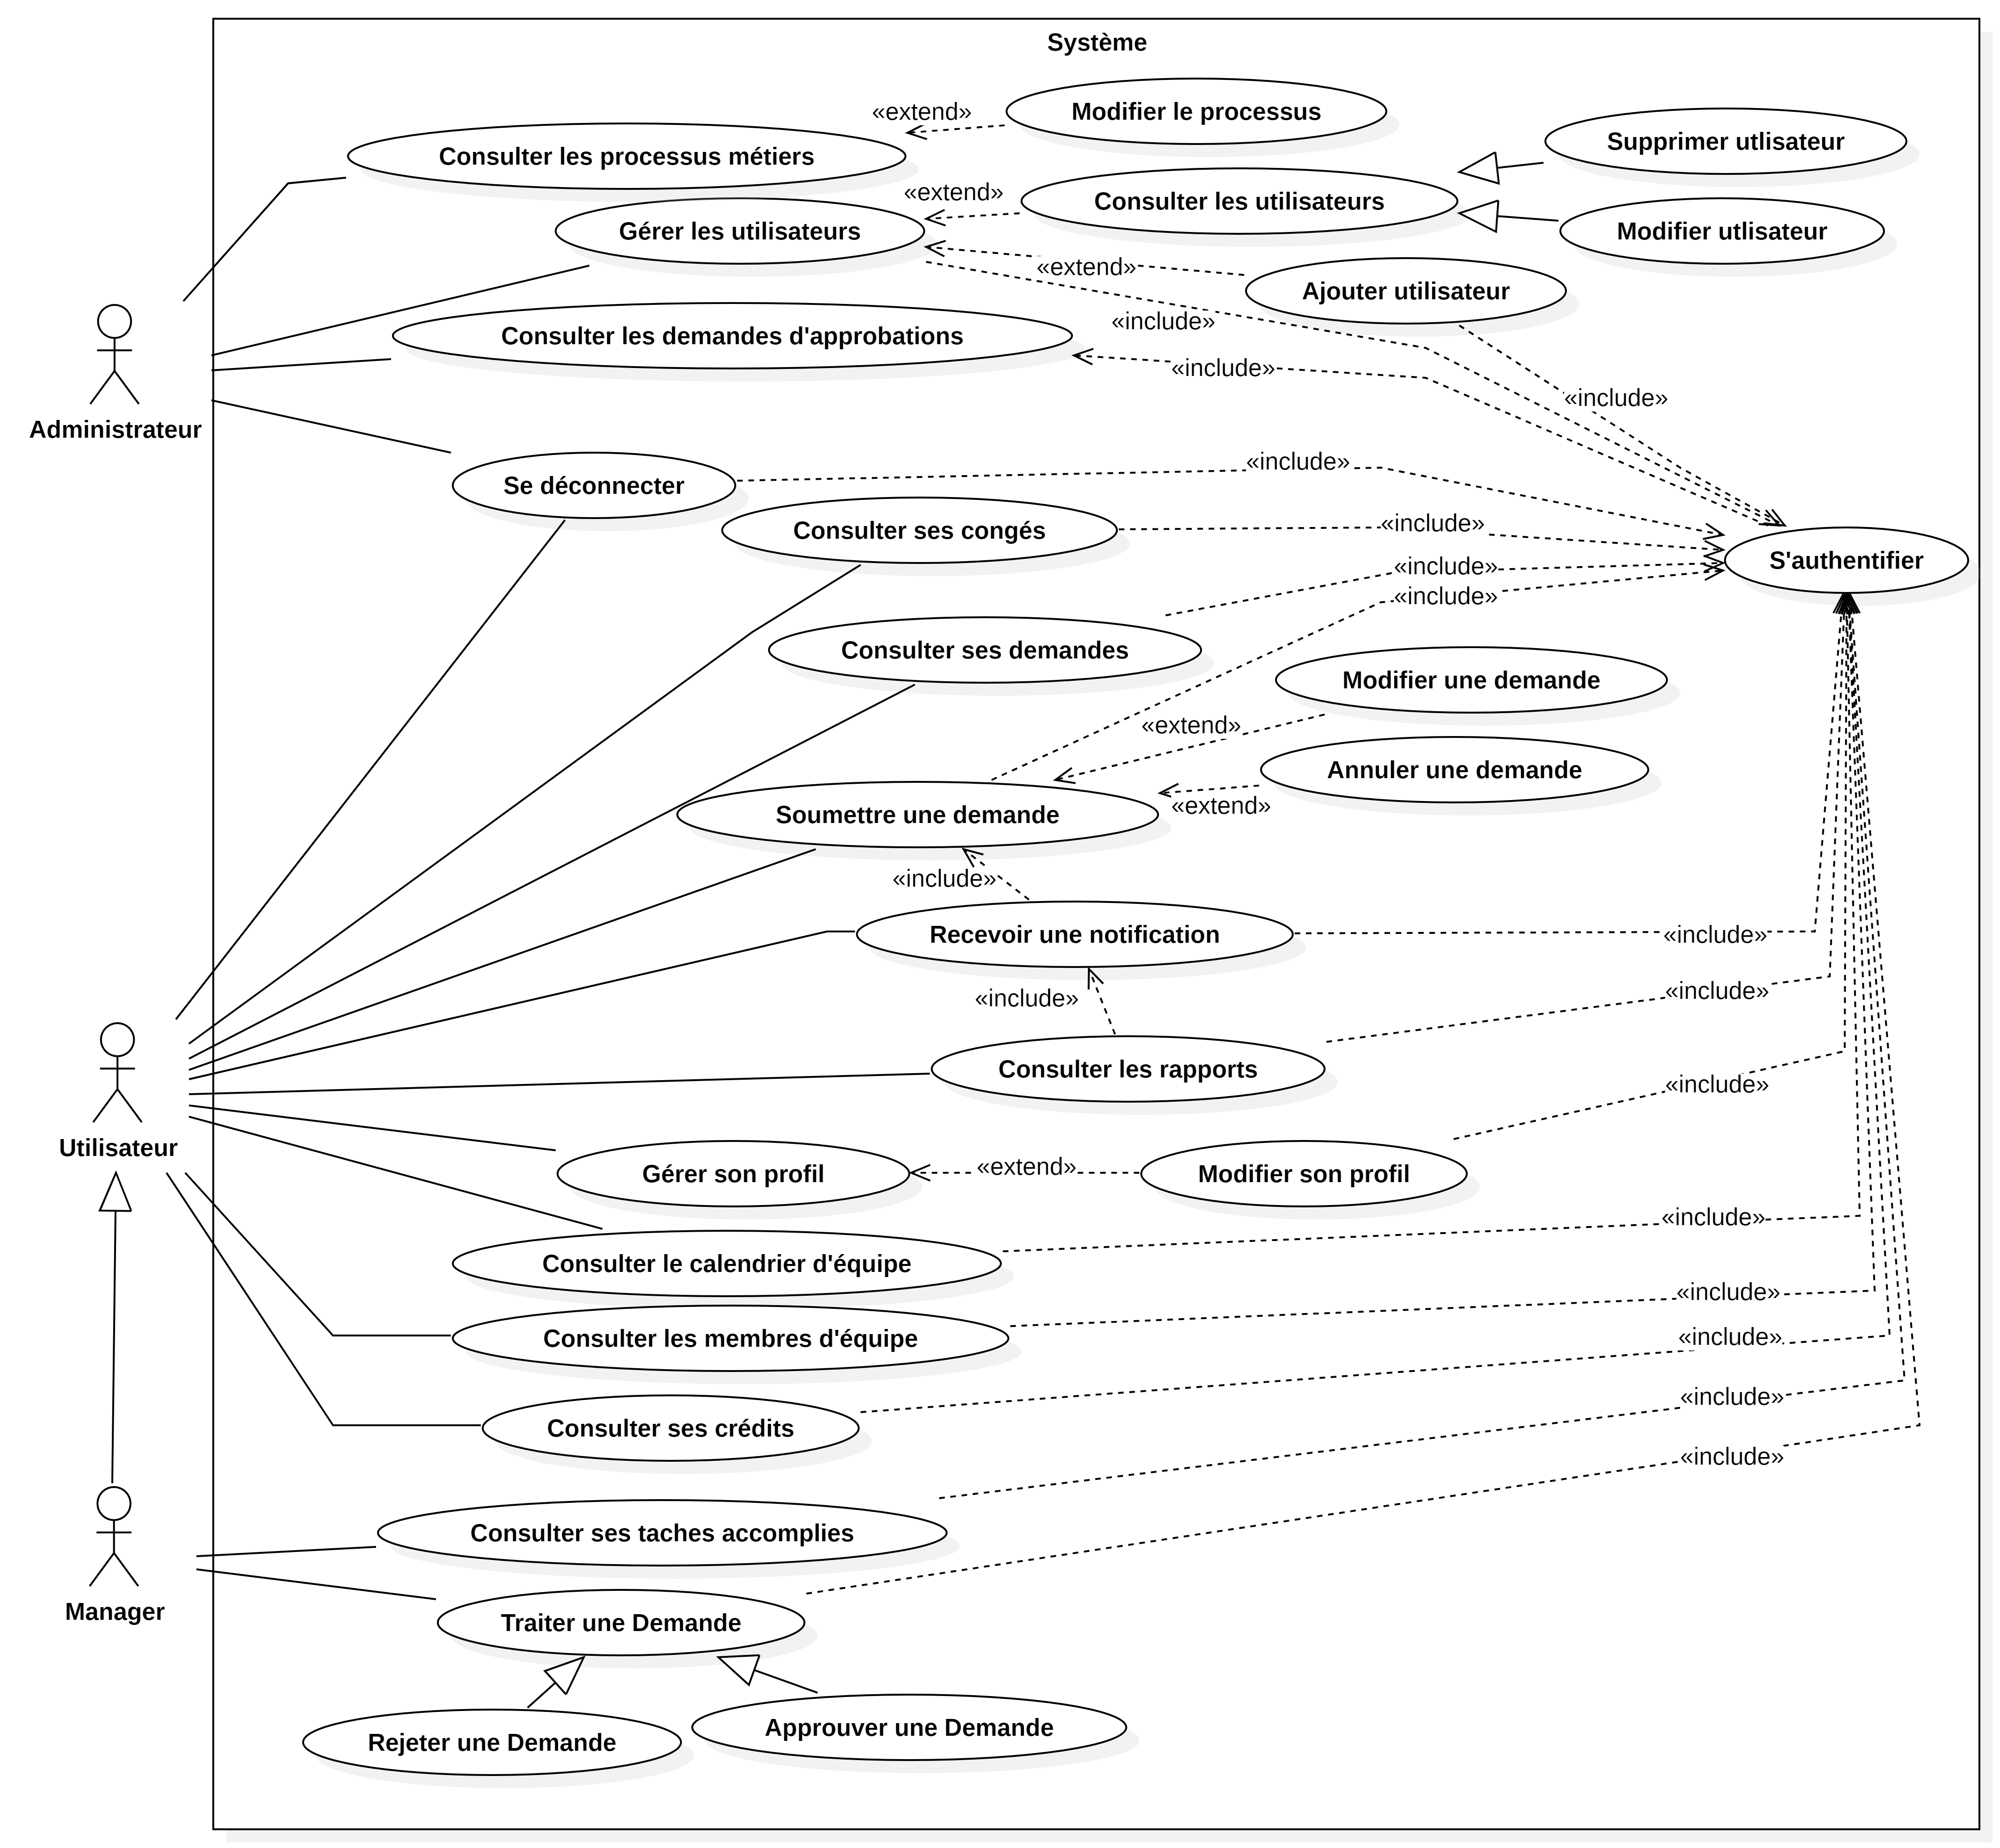
\includegraphics[width=20cm]{images/UseCaseDiagram.jpg}
\caption{Diagramme de cas d'utilisation globale}
\label{usecaseDiagram}
\end{adjustwidth}
\end{figure}
\newpage
\section{Diagramme de classe global}
Le diagramme de classe globale illustré dans la figure \ref{classDiagram} montre la constitution du système
à l’aide de la modélisation de ses classes, ses attributs, ses opérations et l’identification
des relations entre ses objets.
\begin{figure}[H]
\begin{adjustwidth}{-2cm}{-2cm} % reduce left and right margins locally
\centering
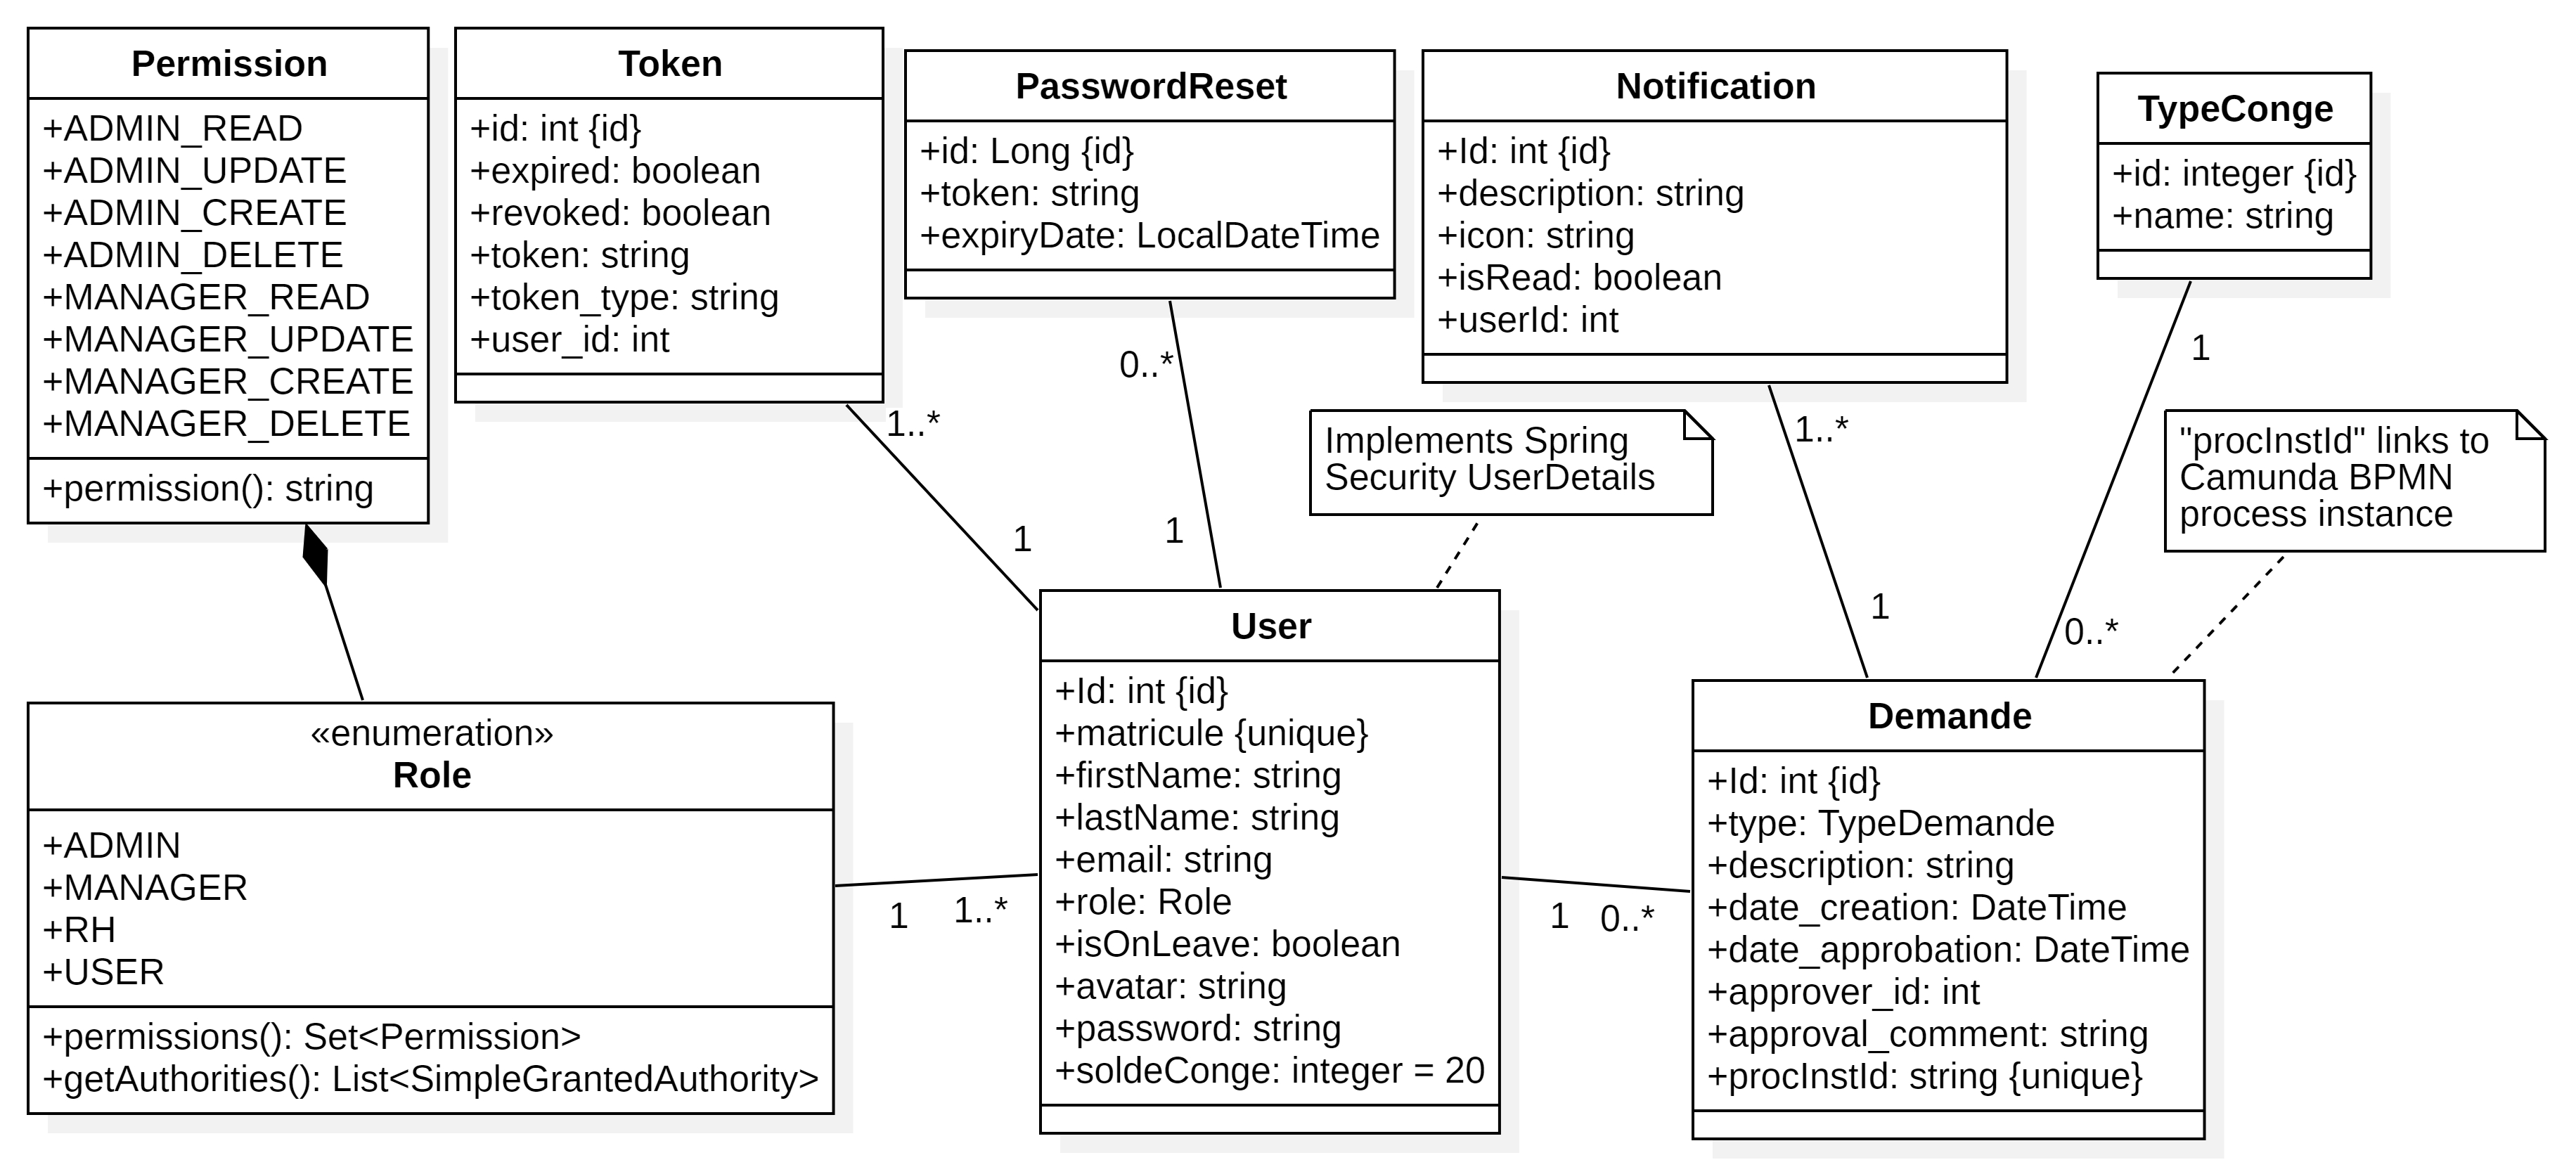
\includegraphics[width=21cm]{images/ClassDiagram.jpg}
\caption{Diagramme de classe globale}
\label{classDiagram}
\end{adjustwidth}
\end{figure}
\section{Backlog du Produit}
Le backlog du produit est un ensemble de tâches priorisées qui caractérise un produit. C'est l'un des éléments indispensables de la méthodologie Scrum. C'est l’outil de travail du Product Owner.\\
Ce qui nous mène à le modéliser dans le tableau \ref{tab:backlog_part1} et \ref{tab:backlog_part2} \cite{}:
\newpage
\begin{table}[h!]
\vspace*{-1.5cm}
\begin{adjustwidth}{-3cm}{-2.7cm}
\centering
\renewcommand{\arraystretch}{1.1}
\begin{tabular}{|p{0.18\textwidth}|p{0.24\textwidth}|p{0.40\textwidth}|p{0.08\textwidth}|}
\hline
\textbf{Sprint} & \textbf{User Story} & \textbf{Description} & \textbf{Priorité} \\
\hline
\multirow{4}{*}{\parbox{0.18\textwidth}{\raggedright Sprint 1 : Accès et Administration de Base}} 
    & \textbullet\ S'authentifier & \textbullet\ \raggedright Permet à tous les utilisateurs d’accéder à la plateforme via nom d’utilisateur et mot de passe. & 1 \\
    & \textbullet\ Se déconnecter & \textbullet\ \raggedright Permet aux utilisateurs de quitter le système après vérification des coordonnées. & 1 \\
    & \textbullet\ Gérer les utilisateurs & \textbullet\ \raggedright L’Administrateur peut ajouter, consulter, modifier et supprimer des utilisateurs. & 1 \\
    & \textbullet\ Mise en place et configuration de Camunda & \textbullet\ \raggedright Permet de configurer et d’intégrer le moteur Camunda dans l’application Spring Boot pour orchestrer les processus métiers. & 1 \\
\hline
\multirow{6}{*}{\parbox{0.18\textwidth}{\raggedright Sprint 2 : Gestion des Demandes}} 
    & \textbullet\ Gérer son profil & \textbullet\ \raggedright Chaque acteur modifie ses informations personnelles (mot de passe, e-mail, etc.). & 2 \\
    & \textbullet\ Réinitialiser son mot de passe & \textbullet\ \raggedright En cas d’oubli, l’utilisateur peut réinitialiser son mot de passe via un lien sécurisé. & 2 \\
    & \textbullet\ Soumettre une demande & \textbullet\ \raggedright Les Utilisateurs, Managers et RH soumettent des demandes (congés, absences, etc.). & 2 \\
    & \textbullet\ Consulter ses demandes & \textbullet\ \raggedright Les Utilisateurs, Managers et RH consultent l’historique de leurs demandes. & 2 \\
    & \textbullet\ Consulter ses congés & \textbullet\ \raggedright Les Utilisateurs, Managers et RH consultent leurs congés et leur solde. & 2 \\
    & \textbullet\ Traiter une demande & \textbullet\ \raggedright Les Managers et RH valident ou rejettent les demandes soumises. & 2 \\
\hline
\multirow{5}{*}{\parbox{0.18\textwidth}{\raggedright Sprint 3 : Suivi et Supervision}} 
    & \textbullet\ Recevoir une notification & \textbullet\ \raggedright Les Utilisateurs, Managers et RH reçoivent des alertes sur des actions importantes. & 2 \\
    & \textbullet\ Consulter les processus métiers & \textbullet\ \raggedright L’Administrateur consulte les processus métiers définis dans le système. & 3 \\
    & \textbullet\ Consulter les demandes d’approbation & \textbullet\ \raggedright L’Administrateur accède aux demandes soumises pour consultation. & 3 \\
    & \textbullet\ Consulter les membres de l’équipe & \textbullet\ \raggedright Les Utilisateurs, Managers et RH accèdent aux infos des membres de leur équipe. & 3 \\
    & \textbullet\ Consulter ses crédits & \textbullet\ \raggedright Les Utilisateurs, Managers et RH vérifient leur solde de congés ou crédits. & 2 \\
\hline
\end{tabular}
\caption{Backlog du Produit - Partie 1}
\label{tab:backlog_part1}
\end{adjustwidth}
\end{table}

\clearpage

\begin{table}[h!]
\vspace*{-1.5cm}
\begin{adjustwidth}{-3cm}{-2.7cm}
\centering
\renewcommand{\arraystretch}{1.1}
\begin{tabular}{|p{0.18\textwidth}|p{0.24\textwidth}|p{0.40\textwidth}|p{0.08\textwidth}|}
\hline
\textbf{Sprint} & \textbf{User Story} & \textbf{Description} & \textbf{Priorité} \\
\hline
\multirow{5}{*}{\parbox{0.18\textwidth}{\raggedright Sprint 4 : Analyse et Améliorations}} 
    & \textbullet\ Consulter le calendrier d’équipe & \textbullet\ \raggedright Les Utilisateurs, Managers et RH consultent les absences et événements d’équipe. & 3 \\
    & \textbullet\ Consulter les tâches accomplies & \textbullet\ \raggedright Les Managers et RH suivent les tâches réalisées par leurs subordonnés. & 3 \\
    & \textbullet\ Consulter les rapports & \textbullet\ \raggedright Les Utilisateurs, Managers et RH consultent des rapports sur leurs activités. & 4 \\
    & \textbullet\ Exporter les rapports & \textbullet\ \raggedright Permet d’exporter les rapports (PDF, Excel) pour une utilisation hors ligne. & 4 \\
    & \textbullet\ Implémentation d’un chatbot & \textbullet\ \raggedright Permet de développer et d’intégrer un chatbot dans l’application pour assister les utilisateurs dans leurs interactions (consultation, soumission de demandes, etc.). & 4 \\
\hline
\multirow{4}{*}{\parbox{0.18\textwidth}{\raggedright Sprint 5 : Déploiement et Pipeline DevOps}} 
    & \textbullet\ Déployer l’application & \textbullet\ \raggedright Permet de déployer l’application sur un serveur ou une plateforme cible. & 5 \\
    & \textbullet\ Configurer le pipeline CI/CD & \textbullet\ \raggedright Met en place un pipeline d’intégration et de déploiement continus pour automatiser les mises à jour. & 5 \\
    & \textbullet\ Surveiller le déploiement & \textbullet\ \raggedright Les administrateurs vérifient l’état et les performances de l’application déployée. & 5 \\
    & \textbullet\ Gérer les versions & \textbullet\ \raggedright Permet de suivre et de gérer les différentes versions de l’application déployée. & 5 \\
\hline
\end{tabular}
\caption{Backlog du Produit - Partie 2}
\label{tab:backlog_part2}
\end{adjustwidth}
\end{table}
\section{Planification de projet}
Cette section a pour objectif de présenter la planification de notre projet. Pour ce faire, nous utiliserons un diagramme de Gantt qui permettra de visualiser les différentes étapes du projet sous forme de tâches à réaliser, facilitant ainsi le suivi et l’organisation du travail.
\subsection{Diagramme de Gantt}
Le diagramme de Gantt présenté par la figure \ref{fig:diagantt} nous permet de visualiser les différentes tâches ainsi que leurs durées.
\newpage
\begin{figure}[H]
\vspace*{-1.8cm}
     \centering
  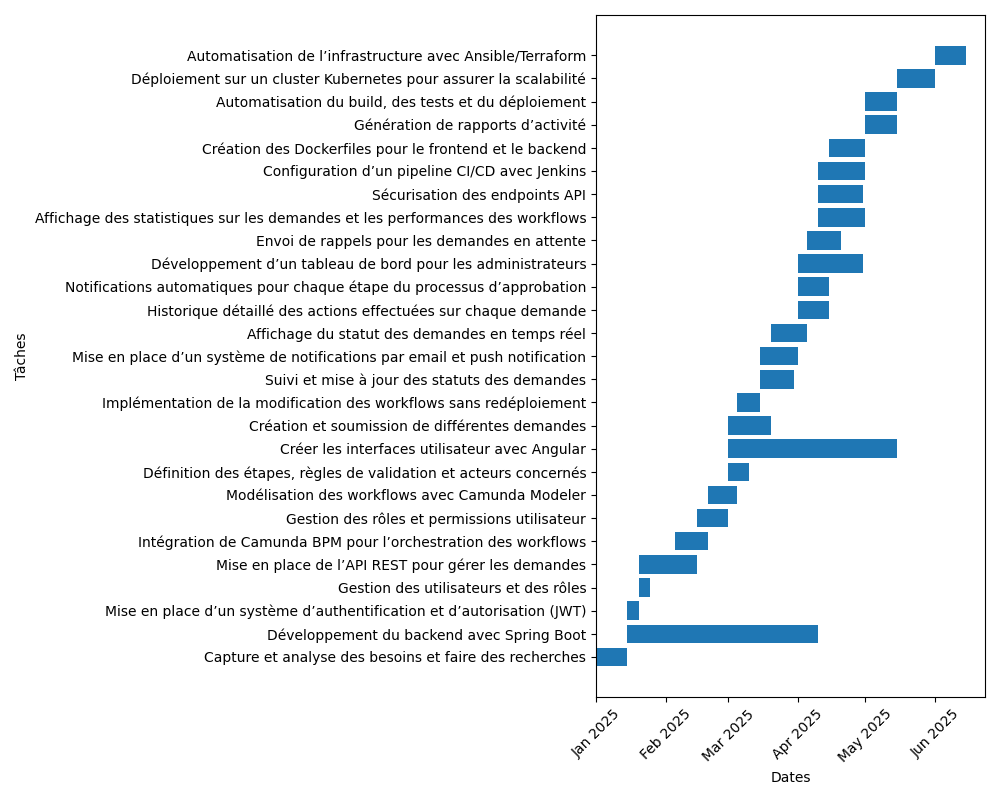
\includegraphics[scale=0.6]{images/gantt.png}
        \caption{Diagramme de Gantt} 
  \label{fig:diagantt}
 \end{figure}

%à ajouter le diagramme le Gantt 
\section{Environnement de travail}
Dans cette section, nous examinerons les différentes outils technologiques adoptées dans le cadre de ce projet.
\subsection{Environnement materiel}
Durant ce projet,nous avons utilisé deux machines pour bien mener notre projet.Les caractéristiques techniques de ces machines sont présentés dans le tableau \ref{tab:specs}.

\begin{table}[h!]
\centering
\caption{Spécifications des machines utilisées}
\label{tab:specs}
\begin{tabularx}{\linewidth}{|X|X|X|}
\hline
\textbf{} & \textbf{Machine 1} & \textbf{Machine 2} \\
\hline
\textbf{Marque} & Gigabyte AERO 15 & Lenovo IdeaPad \\
\hline
\textbf{Système d’exploitation} & Windows 11 64 bit & Windows 10 64 bit \\
\hline
\textbf{Processeur} & I7-11800H 2.3 GHz & I7-9750H 2.6 GHz \\
\hline
\textbf{RAM} & 16 GB 3200MHz & 8 GB \\
\hline
\textbf{Disque Dur} & 1 TB & 500 GB \\
\hline
\end{tabularx}
\end{table}
\newpage
\subsection{Environnement logiciel}
Dans cette section, nous présentons l’environnement logiciel utilisé dans ce projet :

\begin{itemize}
 \item \textbf{Git}Dont le logo est présenté dans la figure \ref{fig:git}, cet outil constitue un système de gestion de versions distribué. Il permet de tracer l’évolution des fichiers et des répertoires d’un projet, d’accéder à des versions précédentes et de consulter en détail l’historique des modifications réalisées.
 \begin{figure}[h]
    \centering
    
\includegraphics[width=2.5cm]{images/git.png}
    \caption{Logo de Git}
    \label{fig:git}
\end{figure}
\item \textbf{Github}:Dont le logo est exposé dans la figure \ref{fig:gituhbl}, 
 est une plateforme collaborative basée sur Git, utilisée pour héberger du code, suivre les changements et faciliter le travail d’équipe sur des projets de développement logiciel.
 \begin{figure}[h]
    \centering
    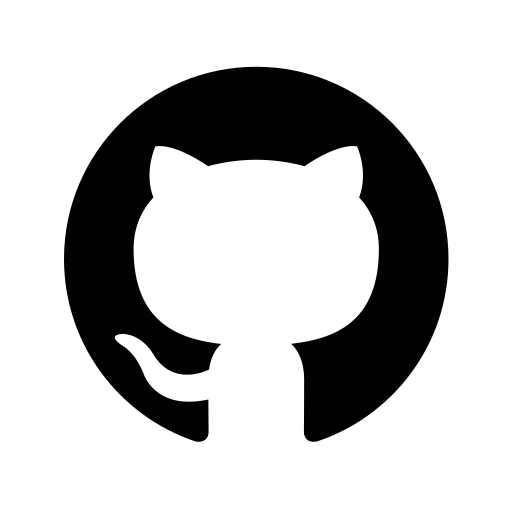
\includegraphics[width=2.2cm]{images/githubl.png}
    \caption{Logo de Github}
    \label{fig:gituhbl}
\end{figure}
\item \textbf{WampServer}:Dont le logo est illustré dans la figure \ref{fig:wamp}, WampServer est un environnement de développement web local pour Windows. Il regroupe Apache, MySQL et PHP, permettant aux développeurs de tester et d’exécuter des applications web en local avant leur mise en production.
 \begin{figure}[h]
    \centering
    
\includegraphics[width=1.8cm]{images/WampServer.png}
    \caption{Logo de WampServer}
    \label{fig:wamp}
\end{figure}
\newpage
\item \textbf{phpMyAdmin}:Dont le logo est représenté dans la figure \ref{fig:phpmyadmin}, phpMyAdmin est une interface web permettant d’administrer facilement des bases de données MySQL ou MariaDB. Il offre aux utilisateurs un accès simplifié pour gérer les tables, exécuter des requêtes SQL, importer ou exporter des données, le tout sans avoir à utiliser la ligne de commande.
 \begin{figure}[h]
    \centering
    
\includegraphics[width=2.9cm]{images/phpmyadmin.png}
    \caption{Logo de phpMyAdmin}
    \label{fig:phpmyadmin}
\end{figure}
\item \textbf{Visual Studio Code (VSCode)}:Représenté dans la figure \ref{fig:vscode}, VSCode est un éditeur de code source léger et extensible, populaire pour le développement Angular. Il offre une riche palette d’extensions, telles que des outils de linting, de débogage, et des intégrations Git, ce qui le rend idéal pour travailler sur des applications JavaScript et TypeScript, comme celles développées avec Angular.
 \begin{figure}[h]
    \centering
    
\includegraphics[width=1.6cm]{images/vscode.png}
    \caption{Logo de VSCode}
    \label{fig:vscode}
\end{figure}
\item \textbf{IntelliJ IDEA}:Représenté dans la figure \ref{fig:intellij}, IntelliJ IDEA est un environnement de développement intégré (IDE) robuste, principalement utilisé pour le développement d'applications Java, telles que celles créées avec Spring. Il offre des fonctionnalités avancées comme la gestion des dépendances, le débogage intégré, et la prise en charge complète de Spring, ce qui facilite le développement et le déploiement d’applications Spring Boot.
 \begin{figure}[h]
    \centering
    
\includegraphics[width=1.8cm]{images/intellij.png}
    \caption{Logo de IntelliJ}
    \label{fig:intellij}
\end{figure}
\newpage
\end{itemize}
\section{Choix technologiques}
\begin{itemize}
 \subsection{Frontend}
\item \textbf{Angular}:Représenté dans la figure \ref{fig:angular}, Angular est un framework de développement web permettant de créer des applications web dynamiques et interactives.
 \begin{figure}[h]
    \centering
    
\includegraphics[width=1.8cm]{images/angular.png}
    \caption{Logo d'Angular}
    \label{fig:angular}
\end{figure}
 \subsection{Backend}
\item \textbf{Spring Boot}:Représenté dans la figure \ref{fig:SpringBoot}, Spring Boot est un framework Java qui facilite le développement d’applications Spring en simplifiant la configuration et le déploiement, tout en offrant des outils prêts à l’emploi comme un serveur embarqué et une sécurité intégrée.
 \begin{figure}[h]
    \centering
    
\includegraphics[width=1.6cm]{images/SpringBoot.png}
    \caption{Logo de Spring Boot}
    \label{fig:SpringBoot}
\end{figure}
\subsection{Workflow}
\item \textbf{Camunda}:Dont le logo est représenté dans la figure \ref{fig:camunda}, Camunda est une plateforme open-source de gestion des processus métier (BPMN), de gestion des décisions (DMN) et de gestion des cas (CMMN). Camunda est particulièrement utilisé pour l'orchestration des workflows complexes et s'intègre facilement dans des architectures Java et microservices.
 \begin{figure}[h]
    \centering
    
\includegraphics[width=1.6cm]{images/camunda.png}
    \caption{Logo de Camunda}
    \label{fig:camunda}
\end{figure}
\newpage
\subsection{Base de données}
\item \textbf{MySQL}:Représenté dans la figure \ref{fig:MySQL}, MySQL est un système de gestion de bases de données relationnelles open-source. Il permet de stocker, gérer et interroger des données de manière structurée à l'aide de SQL.
 \begin{figure}[h]
    \centering
    
\includegraphics[width=2.3cm]{images/MySQL.png}
    \caption{Logo de MySQL}
    \label{fig:MySQL}
\end{figure}
\subsection{CI/CD}
\item \textbf{ArgoCD}:Représenté dans la figure \ref{fig:ArgoCD}, ArgoCD est un outil open-source d'intégration et de déploiement continu (CI/CD) spécialement conçu pour Kubernetes. Il permet de déployer et gérer des applications dans des environnements Kubernetes en suivant la méthodologie GitOps.
 \begin{figure}[h]
    \centering
    
\includegraphics[width=1.6cm]{images/ArgoCD.png}
    \caption{Logo d'ArgoCD}
    \label{fig:ArgoCD}
\end{figure}
\subsection{Conteneurisation}
\item \textbf{Docker}:Représenté dans la figure \ref{fig:docker}, Docker est une plateforme open-source permettant de créer, déployer et exécuter des applications dans des conteneurs. Ces conteneurs encapsulent l’application et ses dépendances dans un environnement léger et portable.
 \begin{figure}[h]
    \centering
    
\includegraphics[width=2.5cm]{images/docker.png}
    \caption{Logo de Docker}
    \label{fig:docker}
\end{figure}
\newpage
\subsection{Orchestration}
\item \textbf{Kubernetes}:Représenté dans la figure \ref{fig:kubernetes}, Kubernetes est un système open-source d'orchestration de conteneurs qui automatise le déploiement, la gestion, la mise à l’échelle et l’administration des applications conteneurisées. Il permet de gérer efficacement les clusters de conteneurs Docker, offrant des fonctionnalités telles que l’autoscaling, la gestion des ressources et le monitoring des applications.
 \begin{figure}[h]
    \centering
    
\includegraphics[width=1.6cm]{images/kubernetes.png}
    \caption{Logo de Kubernetes}
    \label{fig:kubernetes}
\end{figure}
\end{itemize}
\section*{Conclusion}
Dans ce deuxième chapitre, nous avons détaillé les besoins fonctionnels et non fonctionnels du projet, ainsi que les différents acteurs et leurs interactions avec le système à travers des diagrammes de cas d'utilisation et de classes globaux. Nous avons également présenté le backlog du produit, structuré en sprints, et défini les priorités pour chaque fonctionnalité.
Nous avons également présenté les choix technologiques retenus pour le développement du projet, couvrant l'environnement matériel, l'environnement logiciel.
Le chapitre suivant sera consacré à la présentation du Sprint 1, qui couvrira les premières étapes du développement, notamment l'accès et l'administration de base du système.




\clearpage

\chapter{Sprint 1 : Accès et administration de base}

\section{Introduction}

Après avoir tracer les grandes lignes de notre projet, concentrons-nous maintenant sur le
premièr sprint. Dans ce qui suit, nous expliquerons chaque fonctionnalité de ce sprint
en detaillant ses différents besoins, ainsi que sa conception .
\section{Backlog de Sprint 1}
Le tableau 3.1 représente le backlog du premier sprint. Ce tableau détaille les cas d’utilisation, leurs priorités, estimations et tâches associées.
\begin{table}[!ht]
\begin{adjustwidth}{-2cm}{-2cm}
\centering
\caption{Backlog du Sprint 1}
\label{tab:backlog_sprint1}
\begin{tabular}{ | m{9cm} | m{1.2cm} | m{4.5cm} | }
\hline
\cellcolor[rgb]{0.832,0.832,0.832}Cas d'utilisation & \cellcolor[rgb]{0.832,0.832,0.832}Priorité & \cellcolor[rgb]{0.832,0.832,0.832}Tâche \\
\hline
En tant qu’utilisateur ou admin, je peux m’authentifier & 1 & Authentifier l'utlisateur a l'aide du token JWT \\
\hline
En tant qu’utilisateur ou admin, je peux me déconnecter & 1 & Déconnecter l'utilisateur du session \\
\hline
En tant qu’admin, je peux gérer les utilisateurs & 1 & Ajouter, consulter, modifier, supprimer \\
\hline
En tant que développeur, je peux configurer et intégrer Camunda & 1 & Configurer dépendances Camunda \\
\hline
\end{tabular}
\end{adjustwidth}
\end{table}
\newpage
\section{Raffinement des cas d'utilisation}
Cette section raffine les cas d’utilisation du Sprint 1 en identifiant les acteurs et en détaillant chaque cas d’utilisation.

\subsection{Identification des acteurs du premier sprint}
Les acteurs de ce sprint sont : \\
\textbf{Administrateur} : Acteur principal, il peut s’authentifier, se déconnecter, et gérer les utilisateurs (ajouter, consulter, modifier, supprimer). \\
\textbf{Utilisateur} : Tout acteur ayant un compte, pouvant s’authentifier et se déconnecter. \\
\textbf{Développeur} : Acteur technique qui configure le moteur Camunda dans l’application pour activer les workflows.

\subsection{Raffinement du cas d'utilisation <<S'authentifier>>}
La figure~\ref{fig:auth_diagram} illustre le diagramme de cas d’utilisation « S’authentifier ».
\begin{figure}[h]
     \centering
     \fbox{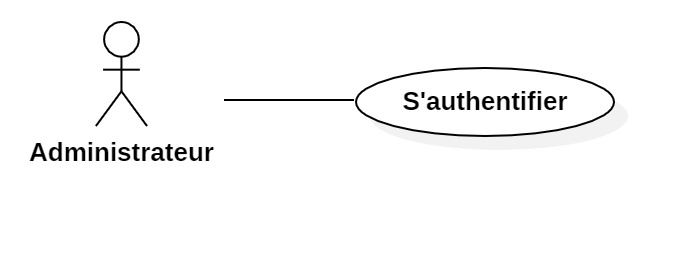
\includegraphics[width=10cm]{images/sauthentifier.jpg}}
     \caption{Diagramme du cas d'utilisation <<S'authentifier>>}
     \label{fig:auth_diagram}
\end{figure}\\
Le tableau \ref{tab:rafLogin} illustre la description détaillée du cas d'utilisation `s’authentifier`.
\begin{table}[!h]
\centering
\caption{Description textuelle du cas d’utilisation «S’authentifier»}
\renewcommand{\arraystretch}{1.2}
\begin{tabular}{|p{4.2cm}|p{11cm}|}
\hline
\textbf{Cas d'utilisation} & S'authentifier \\
\hline
\textbf{Acteur} & Utilisateur \\
\hline
\textbf{Pré-conditions} & Système en marche, utilisateur inscrit \\
\hline
\textbf{Post-conditions} & Utilisateur authentifié, redirigé selon son rôle \\
\hline
\textbf{Scénario de base} & 
1. Affichage de l’interface de connexion \newline
2. Saisie de l’email et du mot de passe \newline
3. Clic sur « Se connecter » \newline
4. Vérification des identifiants \newline
5. Redirection vers l’accueil \\
\hline
\textbf{Exceptions} & 
- Erreur si identifiants incorrects \newline
- Redirection vers l’authentification si le token JWT est expiré \\
\hline
\end{tabular}
\label{tab:rafLogin}
\end{table}
\newpage
\subsection{Raffinement du cas d'utilisation <<Se déconnecter>>}
La figure~\ref{fig:logout_diagram} illustre le diagramme de cas d’utilisation « Se déconnecter ».

\begin{figure}[h]
     \centering
     \fbox{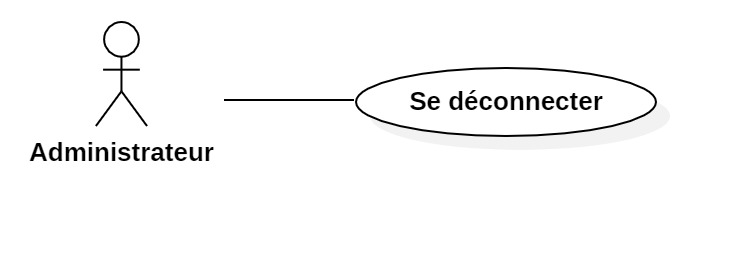
\includegraphics[width=11cm]{images/deconn.jpg}}
     \caption{Diagramme du cas d'utilisation <<Se déconnecter>>}
     \label{fig:logout_diagram}
\end{figure}
Le tableau \ref{tab:rafLogout} illustre la description détaillée du cas d'utilisation `Se déconnecter`.
\begin{table}[!h]
\centering
\caption{Cas d’utilisation : Se déconnecter}
\renewcommand{\arraystretch}{1.2}
\begin{tabular}{|p{4.2cm}|p{11cm}|}
\hline
\textbf{Cas d'utilisation} & Se déconnecter \\
\hline
\textbf{Acteur} & Utilisateur \\
\hline
\textbf{Pré-conditions} & Système en marche, utilisateur connecté \\
\hline
\textbf{Post-conditions} & Utilisateur déconnecté \\
\hline
\textbf{Scénario de base} & 
1. L’utilisateur clique sur « Se déconnecter » \newline
2. Le système redirige vers l’interface d’authentification \\
\hline
\textbf{Exceptions} & 
- Échec de déconnection (erreur API) \\
\hline
\end{tabular}
\label{tab:rafLogout}
\end{table}
\subsection{Raffinement du cas d'utilisation <<Gérer les utilisateurs>>}
La figure~\ref{fig:manage_users_diagram} illustre le diagramme de cas d'utilisation « Gérer les utilisateurs ».

\begin{figure}[h]
     \centering
     \fbox{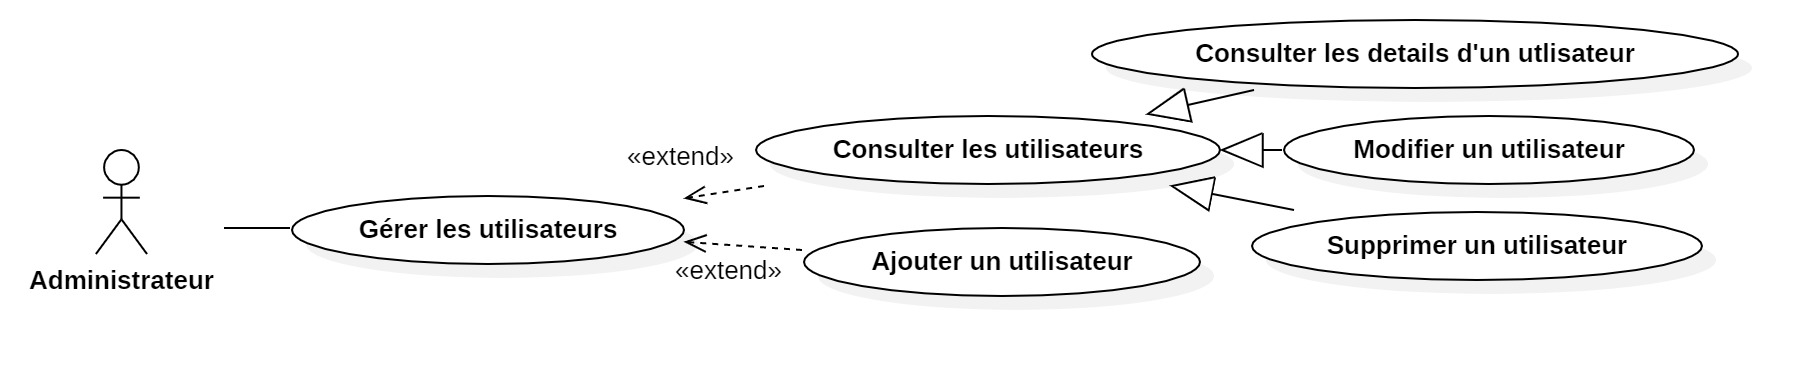
\includegraphics[width=17cm]{images/gererUsers.jpg}}
     \caption{Diagramme du cas d'utilisation <<Gérer les utilisateurs>>}
     \label{fig:manage_users_diagram}
\end{figure}
\newpage
Le tableau~\ref{tab:add_user} illustre la description détaillée du cas d'utilisation « Ajouter un utilisateur ».

\begin{table}[!ht]
\centering
\caption{Description textuelle du cas d’utilisation « Ajouter un utilisateur »}
\label{tab:add_user}
\renewcommand{\arraystretch}{1.2}
\begin{tabular}{|p{4.2cm}|p{11cm}|}
\hline
\textbf{Cas d'utilisation} & Ajouter un utilisateur \\
\hline
\textbf{Acteur} & Admin \\
\hline
\textbf{Pré-conditions} & Le système est en marche. \newline L’admin est authentifié. \\
\hline
\textbf{Post-conditions} & L'utilisateur est ajouté. \\
\hline
\textbf{Scénario de base} & 
1. Le système affiche l’interface d’ajout. \newline
2. L’admin saisit les données du nouvel utilisateur (nom, email, rôle, etc.). \newline
3. L’admin clique sur le bouton « Ajouter ». \newline
4. Le système enregistre les informations. \newline
5. Le système affiche un message de succès. \\
\hline
\textbf{Exceptions} & 
Échec d’ajout (entrées invalides, problème avec l’API POST, ou erreur de base de données). \\
\hline
\end{tabular}
\end{table}


Le tableau~\ref{tab:view_users} illustre la description détaillée du cas d'utilisation « Consulter les utilisateurs ».

\begin{table}[!ht]
\centering
\caption{Description textuelle du cas d’utilisation « Consulter les utilisateurs »}
\label{tab:view_users}
\renewcommand{\arraystretch}{1.2}
\begin{tabular}{|p{4.2cm}|p{11cm}|}
\hline
\textbf{Cas d'utilisation} & Consulter les utilisateurs \\
\hline
\textbf{Acteur} & Admin \\
\hline
\textbf{Pré-conditions} & Le système est en marche. \newline L’admin est authentifié. \\
\hline
\textbf{Post-conditions} & La liste des utilisateurs est consultée. \\
\hline
\textbf{Scénario de base} & 
1. Le système affiche la liste des utilisateurs. \newline
2. L’admin consulte la liste. \\
\hline
\textbf{Exceptions} & 
Échec de consultation (problème avec l’API GET, ou erreur de base de données). \\
\hline
\textbf{Extensions} & 
Modifier un utilisateur. \newline Supprimer un utilisateur. \\
\hline
\end{tabular}
\end{table}

\newpage
Le tableau~\ref{tab:view_user_details} illustre la description détaillée du cas d'utilisation « Consulter les détails d’un utilisateur ».

\begin{table}[!ht]
\centering
\caption{Description textuelle du cas d’utilisation « Consulter les détails d’un utilisateur »}
\label{tab:view_user_details}
\renewcommand{\arraystretch}{1.2}
\begin{tabular}{|p{4.2cm}|p{11cm}|}
\hline
\textbf{Cas d'utilisation} & Consulter les détails d’un utilisateur \\
\hline
\textbf{Acteur} & Admin \\
\hline
\textbf{Pré-conditions} & Le système est en marche. \newline L’admin est authentifié. \\
\hline
\textbf{Post-conditions} & Les informations détaillées de l’utilisateur sont affichées. \\
\hline
\textbf{Scénario de base} & 
1. L’admin clique sue le bouton pour afficher les détails d'un utilisateur depuis la liste. \newline
2. Le système affiche les informations détaillées de l’utilisateur (nom, email, rôle, date de création, etc.). \\
\hline
\textbf{Exceptions} & 
Échec de consultation (problème avec l’API GET, ou erreur de base de données). \\
\hline
\end{tabular}
\end{table}
\vspace{0.5cm}
Le tableau~\ref{tab:update_user} illustre la description détaillée du cas d'utilisation « Modifier un utilisateur ».

\begin{table}[!ht]
\centering
\caption{Description textuelle du cas d’utilisation « Modifier un utilisateur »}
\label{tab:update_user}
\renewcommand{\arraystretch}{1.2}
\begin{tabular}{|p{4.2cm}|p{11cm}|}
\hline
\textbf{Cas d'utilisation} & Modifier un utilisateur \\
\hline
\textbf{Acteur} & Admin \\
\hline
\textbf{Pré-conditions} & Le système est en marche. \newline L’admin est authentifié. \\
\hline
\textbf{Post-conditions} & L'utilisateur est modifié. \\
\hline
\textbf{Scénario de base} & 
1. Le système affiche l’interface de modification. \newline
2. L’admin saisit les nouvelles données. \newline
3. L’admin clique sur le bouton « Modifier ». \newline
4. Le système enregistre les modifications. \newline
5. Le système affiche un message de succès. \\
\hline
\textbf{Exceptions} & 
Échec de modification (problème avec l’API PUT, ou erreur de base de données). \\
\hline
\end{tabular}
\end{table}

\newpage
\vspace*{-1.5cm}
Le tableau~\ref{tab:delete_user} illustre la description détaillée du cas d'utilisation « Supprimer un utilisateur ».

\begin{table}[!ht]
\centering
\caption{Description textuelle du cas d’utilisation « Supprimer un utilisateur »}
\label{tab:delete_user}
\renewcommand{\arraystretch}{1.2}
\begin{tabular}{|p{4.2cm}|p{11cm}|}
\hline
\textbf{Cas d'utilisation} & Supprimer un utilisateur \\
\hline
\textbf{Acteur} & Admin \\
\hline
\textbf{Pré-conditions} & Le système est en marche. \newline L’admin est authentifié. \\
\hline
\textbf{Post-conditions} & L'utilisateur est supprimé. \\
\hline
\textbf{Scénario de base} & 
1. L’admin clique sur le bouton « Supprimer » d’un utilisateur. \newline
2. Le système supprime les données correspondantes. \newline
3. Le système affiche un message de succès. \\
\hline
\textbf{Exceptions} & 
Échec de suppression (problème avec l’API DELETE, ou erreur de base de données). \\
\hline
\end{tabular}
\end{table}
\subsection{Raffinement du cas d'utilisation <<Mise en place et configuration de Camunda>>}
Le tableau~\ref{tab:confCamunda} illustre la description détaillée du cas d'utilisation « Mise en place et configuration de Camunda ».
\begin{table}[!h]
\centering
\caption{Description textuelle du cas d’utilisation «Mise en place et configuration de Camunda»}
\label{tab:confCamunda}
\renewcommand{\arraystretch}{1.2}
\begin{tabular}{|p{4.2cm}|p{11cm}|}
\hline
\textbf{Cas d'utilisation} & Mise en place et configuration de Camunda \\
\hline
\textbf{Acteur} & Développeur \\
\hline
\textbf{Pré-conditions} & 
Le projet backend (Spring Boot) est accessible. \newline
L’environnement de développement est configuré (Java, Maven, IDE). \\
\hline
\textbf{Post-conditions} & Le moteur Camunda est intégré, configuré et fonctionnel dans l’application Spring Boot. \\
\hline
\textbf{Scénario de base} & 
1. Le développeur identifie la version de Camunda compatible avec la version de Spring Boot utilisée dans le projet. \newline
2. Le développeur ajoute les dépendances Camunda nécessaires dans le fichier \texttt{pom.xml}. \newline
3. Le développeur configure les propriétés Camunda dans le fichier \texttt{application.properties}. \newline
4. Le développeur initialise et configure le moteur de workflow dans la classe de configuration Spring. \newline
5. Le développeur crée un processus BPMN simple pour tester l’intégration. \newline
6. Le système valide le bon fonctionnement du moteur. \\
\hline
\textbf{Exceptions} & 
Erreurs d’intégration : dépendances manquantes, mauvaise configuration, problèmes de base de données ou de compatibilité. \\
\hline
\end{tabular}
\end{table}
\newpage
\section{Conception}
La conception est une phase importante pour la bonne réalisation d'un projet.Dans cette partie nous allons exposer la conception des cas d'utilisations de ce sprint qui se traduit par un diagramme de classe globale de ce sprint suivi par les diagrammes de classes et les diagrammes de séquences de chaque cas d'utilisation.
\subsection{Diagramme de classe du sprint 1}
La figure~\ref{fig:class_diagram_sprint1} illustre le diagramme de classe du Sprint 1. Il est formé de :
\begin{itemize}
    \item \textbf{Classe "Permission"} : C’est une énumération qui définit les permissions des différents rôles (ADMIN, MANAGER, etc.).
    \item \textbf{Classe "Role"} : C’est une énumération qui permet d’identifier les rôles des utilisateurs de la plateforme.
    \item \textbf{Classe "Token"} : C’est la classe qui gère les jetons d’authentification des utilisateurs.
    \item \textbf{Classe "User"} : C’est la classe qui représente tous les utilisateurs ayant accès à la plateforme.
    \item \textbf{Interface "Implements Spring Security UserDetails"} : Indique que la classe User implémente cette interface pour gérer l’authentification et l’autorisation.
\end{itemize}
\begin{figure}[h]
     \centering
     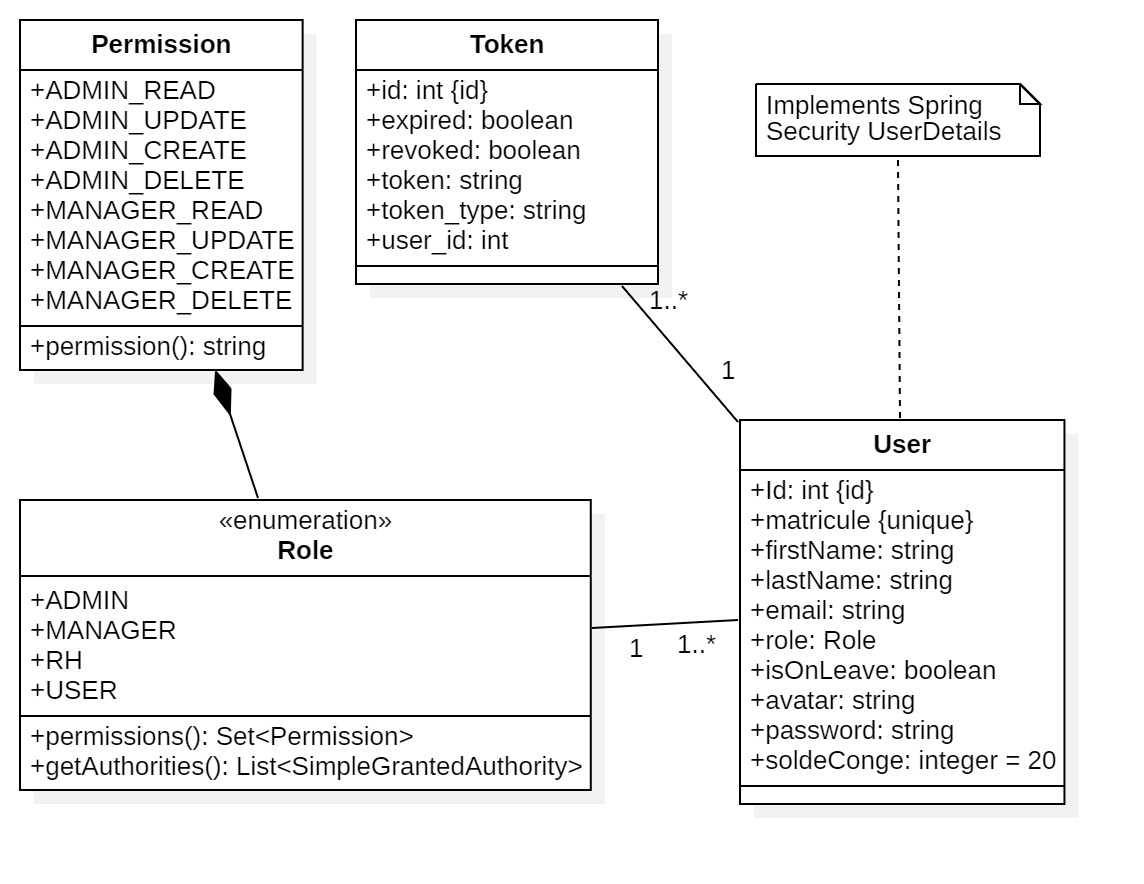
\includegraphics[width=12cm]{images/ClassDiagUs.jpg}
     \caption{Diagramme de classe du sprint 1}
     \label{fig:class_diagram_sprint1}
 \end{figure}
 \newpage
 \subsection{Conception du cas d'utilisation «S'authentifier»}
\subsubsection{Diagramme de classe}
La figure \ref{fig:cauth} illustre le diagramme de classes du cas d’utilisation s'authentifier.
\begin{figure}[h]
     \centering
      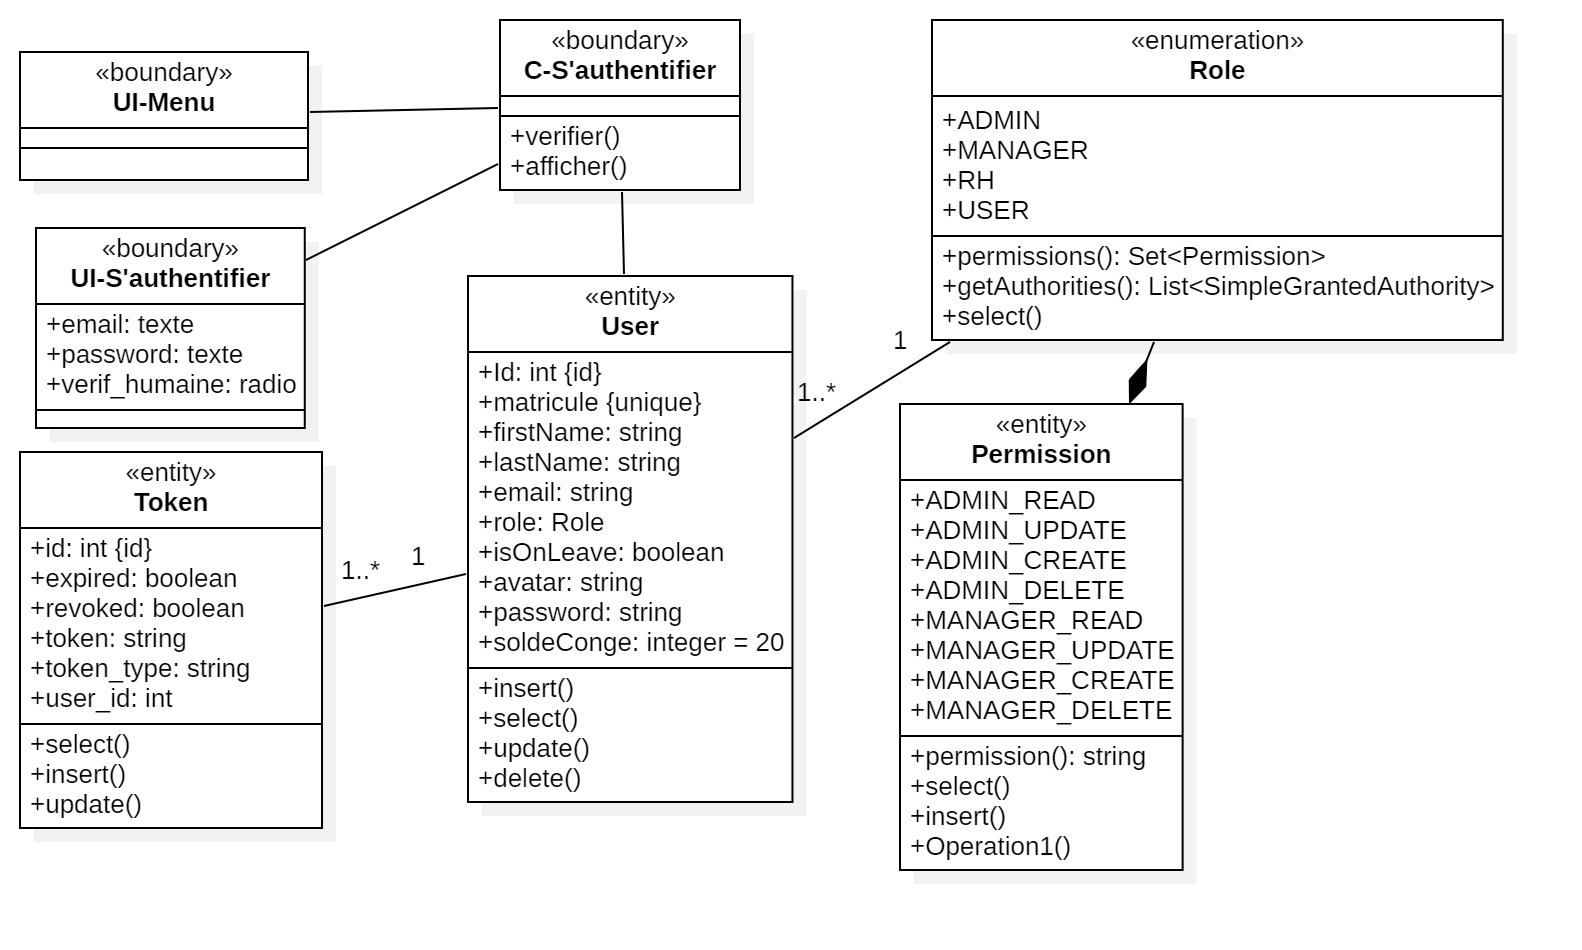
\includegraphics[width=17cm]{images/C-S'authentifier.jpg}
     \caption{Diagramme de classe du cas d'utilisation <<S'authentifier>>}
     \label{fig:cauth}
 \end{figure}
 \subsubsection{Diagramme de séquence}
Au lancement de l'application, une interface d'authentification apparaîtra. Ensuite, les utilisateurs peuvent entrer leurs adresses mail et mots de passe, et vérifier qu'ils ne sont pas un robot (recaptcha), qui seront envoyés via l'interface d'authentification au contrôleur d'authentification, qui à son tour vérifie les informations dans l'entité \textit{Utilisateur}.\\
Si les coordonnées sont correctes, ils seront amenés à un espace approprié selon leurs rôles. Sinon, un message d'erreur d'authentification sera affiché.\\
\noindent La figure~\ref{fig:sauth} modélise le diagramme de séquence du cas d'utilisation « S'authentifier ».
\clearpage
\begin{figure}[h]
     \centering
     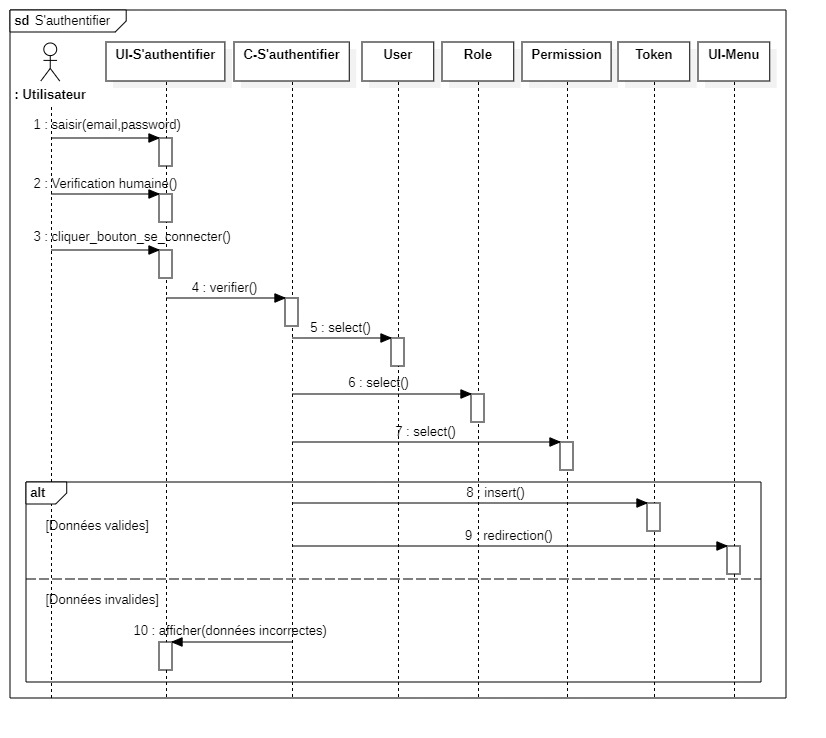
\includegraphics[width=18cm]{images/S-S'authentifier.jpg}
     \caption{Diagramme de séquence du cas d'utilisation <<S'authentifier>>}
     \label{fig:sauth}
\end{figure}

\subsection{Conception du cas d'utilisation «Se déconnecter»}
\subsubsection{Diagramme de classe}
La figure \ref{fig:cdec} illustre le diagramme de classe du cas d’utilisation se déconnecter.
\newpage

\begin{figure}[h]
     \centering
      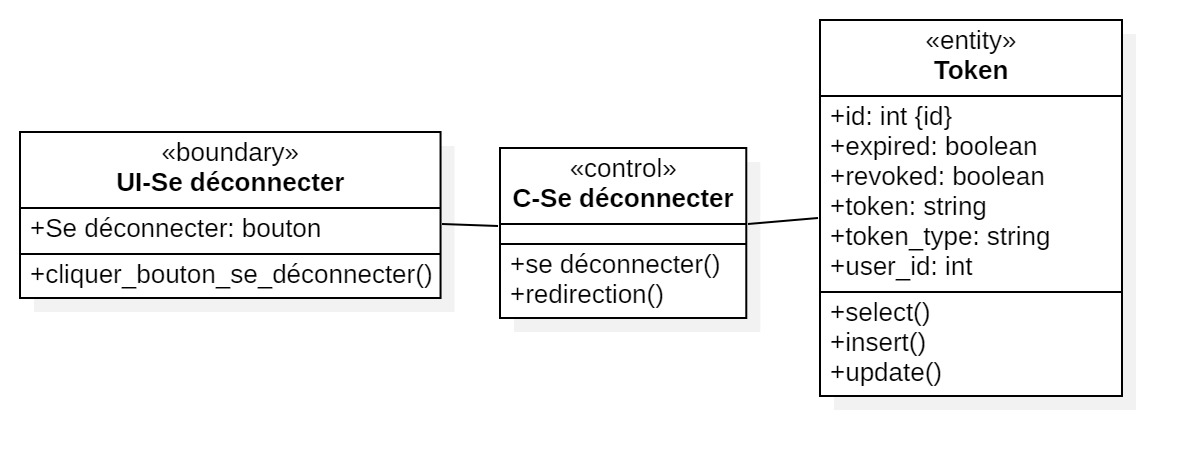
\includegraphics[width=15cm]{images/C-dec.jpg}
     \caption{Diagramme de classe du cas d'utilisation <<Se déconnecter>>}
     \label{fig:cdec}
 \end{figure}
\subsubsection{Diagramme de séquence}
 Si l'utilisateur souhaite se déconnecter, il clique sur le bouton de déconnexion dans le menu. Le système supprime les données obtenues avec l'authentification de l'utilisateur et retire son token. Ce dernier sera finalement redirigé vers l'interface d'authentification.\\
 La figure \ref{fig:sdec} illustre le diagramme de séquence du cas d’utilisation se déconnecter.\\
 \vspace{-0.5cm}
\begin{figure}[h]
     \centering
     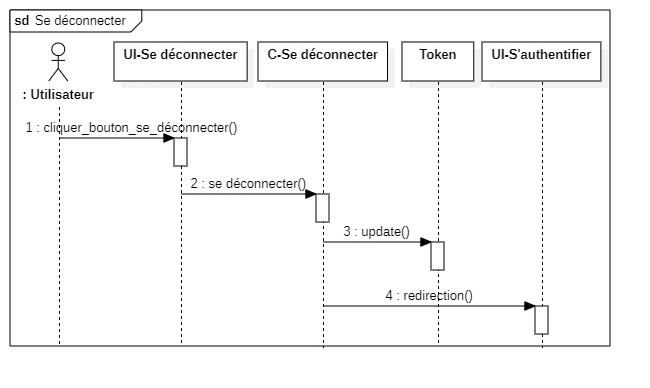
\includegraphics[width=15cm]{images/S-dec.jpg}
     \caption{Diagramme de séquence du cas d'utilisation <<Se déconnecter>>}
     \label{fig:sdec}
\end{figure}
\clearpage
\subsection{Conception du cas d'utilisation «Gérer les utilisateurs»}
\subsubsection{Diagramme de classe}
La figure \ref{fig:cgu} illustre le diagramme de classe du cas d’utilisation gérer les utilisateurs.
\begin{figure}[h]
     \centering
   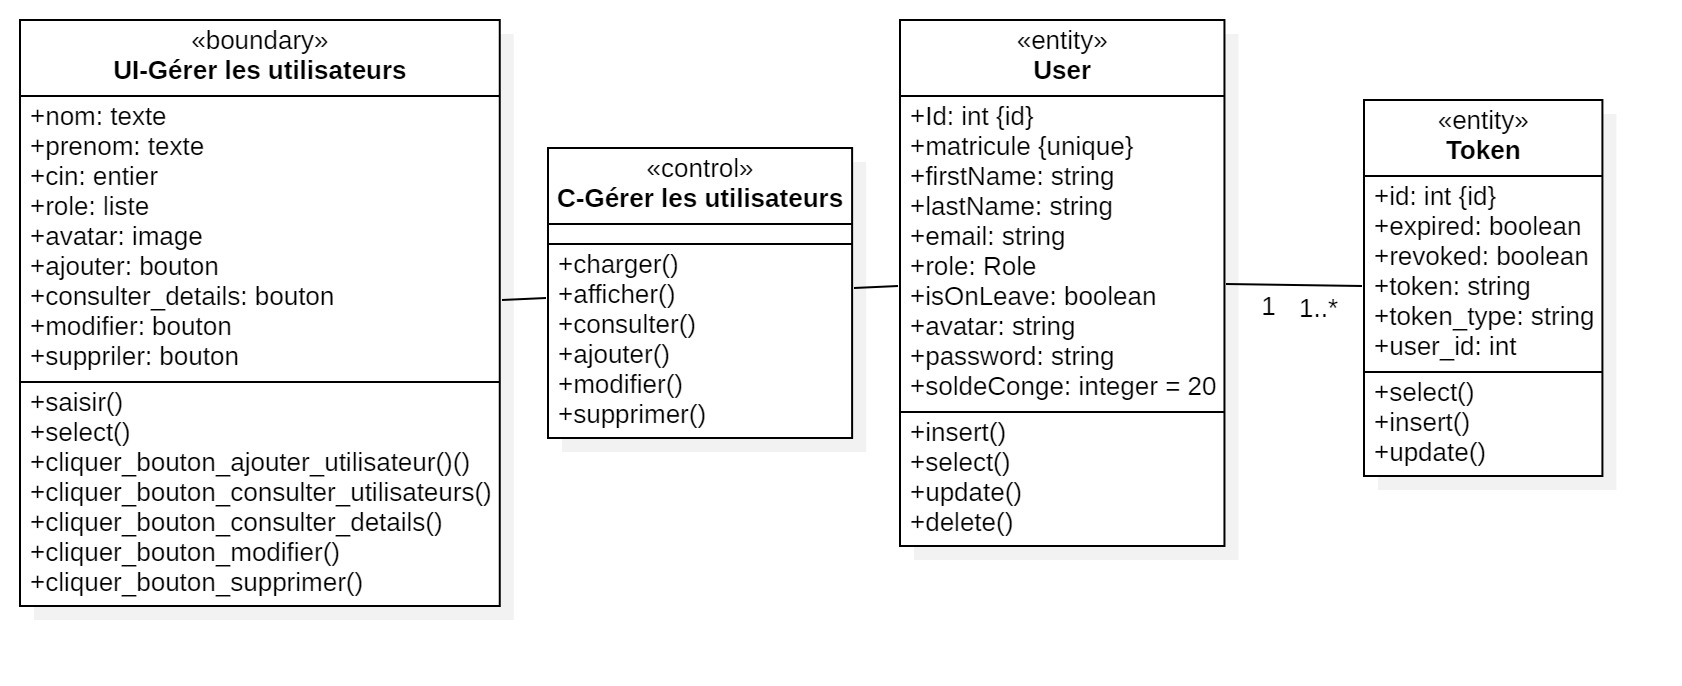
\includegraphics[width=16cm]{images/C-gus.jpg}
     \caption{Diagramme de classe du cas d'utilisation <<Gérer les utilisateurs>>}
     \label{fig:cgu}
 \end{figure}
 \subsubsection{Diagramme de séquence}

Seul l’administrateur dispose des droits nécessaires pour gérer les utilisateurs depuis son interface dédiée. Cette gestion inclut un ensemble d’opérations essentielles telles que l’ajout de nouveaux utilisateurs, la consultation de la liste des utilisateurs existants, l’affichage des détails d’un utilisateur spécifique, la modification de ses informations, ainsi que la suppression d’un compte utilisateur. Toutes ces actions sont déclenchées depuis l’interface d’administration, puis transmises au contrôleur via des requêtes HTTP. Ce dernier assure la logique métier en interagissant avec les entités du système, notamment l’entité "User" pour manipuler les données des utilisateurs, et l’entité "Token" pour révoquer les tokens en cas de suppression d'un utilisateur. \\
La figure~\ref{fig:manage_userss_diagram} illustre le diagramme de séquence du cas d'utilisation « Gérer les utilisateurs ».
\newpage
\vspace*{-3cm} 
\begin{figure}[H]
     \centering
     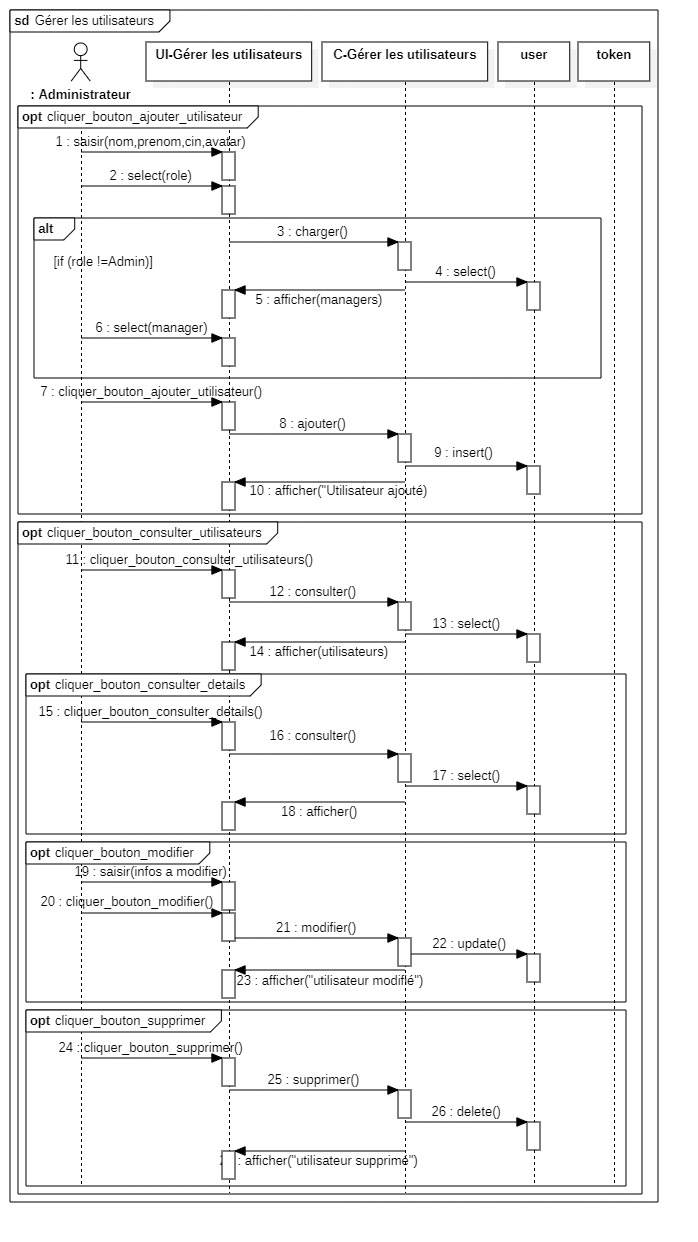
\includegraphics[width=15cm]{images/S-gus.jpg}
     \vspace{-1cm}
     \caption{Diagramme de séquence du cas d'utilisation <<Gérer les utilisateurs>>}
     \label{fig:manage_userss_diagram}
\end{figure}
\section{Réalisation}
Dans cette partie, nous présentons les modules de notre premier sprint en utilisant des captures d’écran.
\subsection{S’authentifier}
L’utilisateur n’est pas autorisé à accéder à l’application, sauf s’il a un compte. Donc, afin d’explorer les fonctionnalités de l’application, l’utilisateur est invité à s’authentifier avec un email et un mot de passe comme le montre la figure \ref{fig:realauth} ci-dessous. L’utilisateur ne peut pas créer un compte puisque les comptes sont attribués par un administrateur.
\begin{figure}[H]
     \centering
     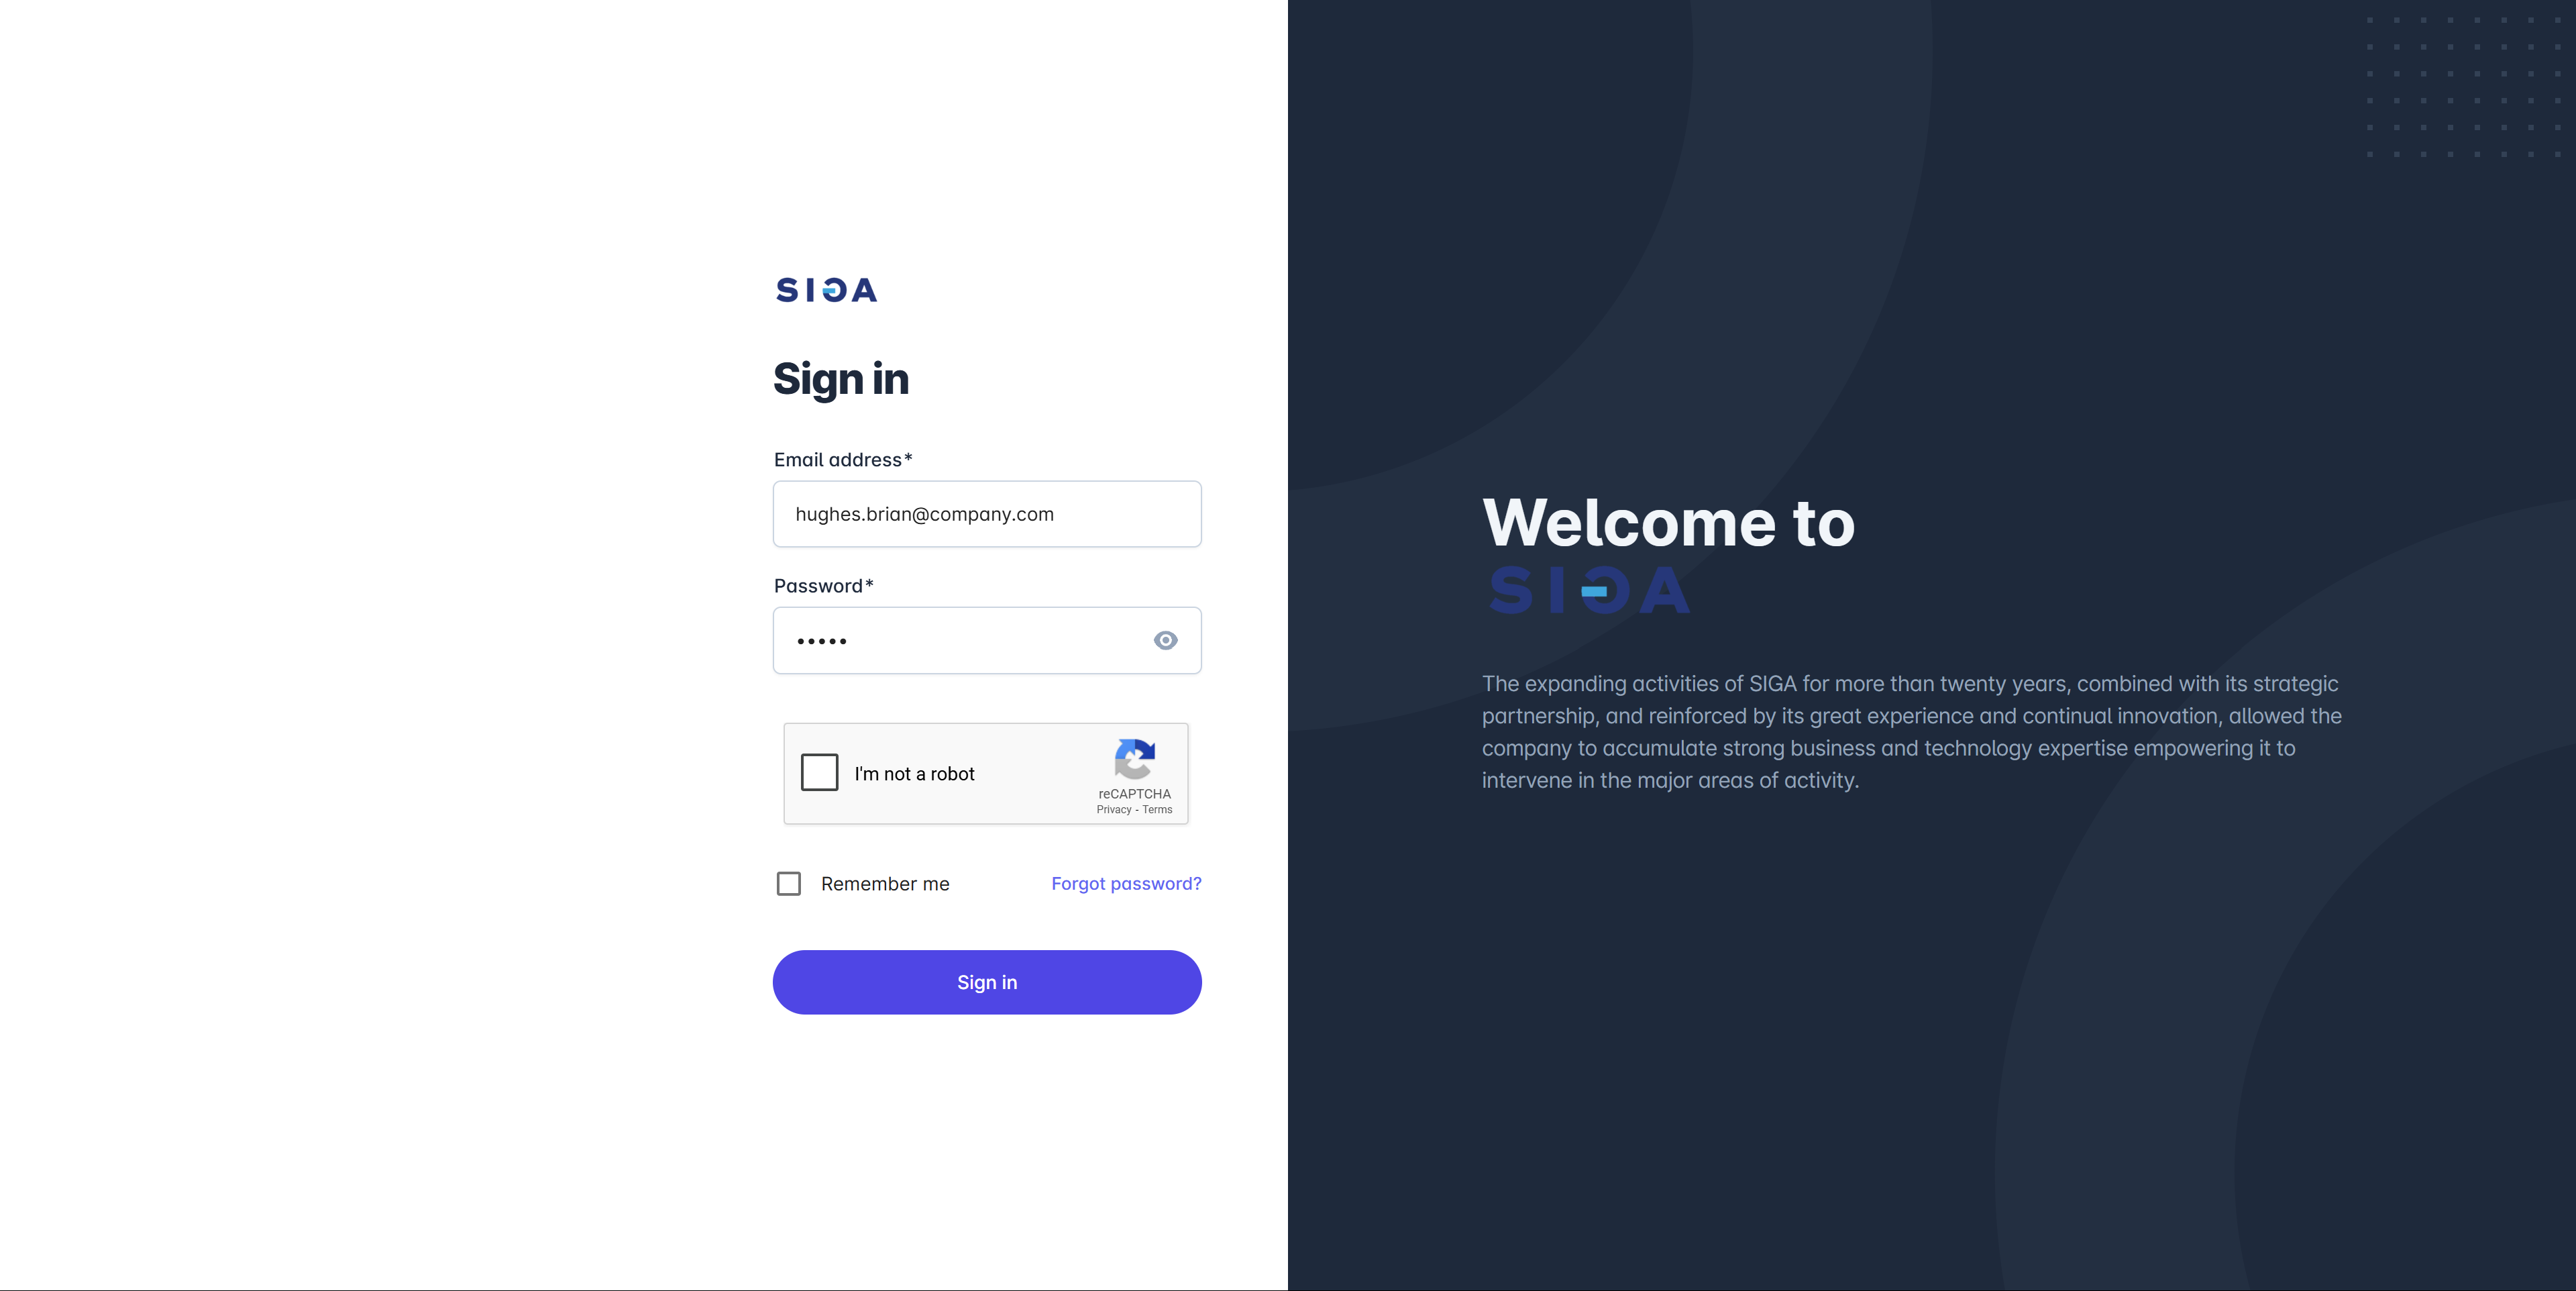
\includegraphics[width=16cm]{images/realisation/login.png}
     \caption{Interface du cas d'utilisation <<S'authentifier>>}
     \label{fig:realauth}
\end{figure}
\subsection{Se déconnecter}
L’utilisateur a la possibilité de se déconnecter de l’application lorsqu’il le souhaite, comme le montre la figure \ref{fig:reallogout}. Cette action met fin à sa session en cours et le redirige vers la page d’authentification.
\newpage
\vspace*{-2cm}
\begin{figure}[H]
     \centering
     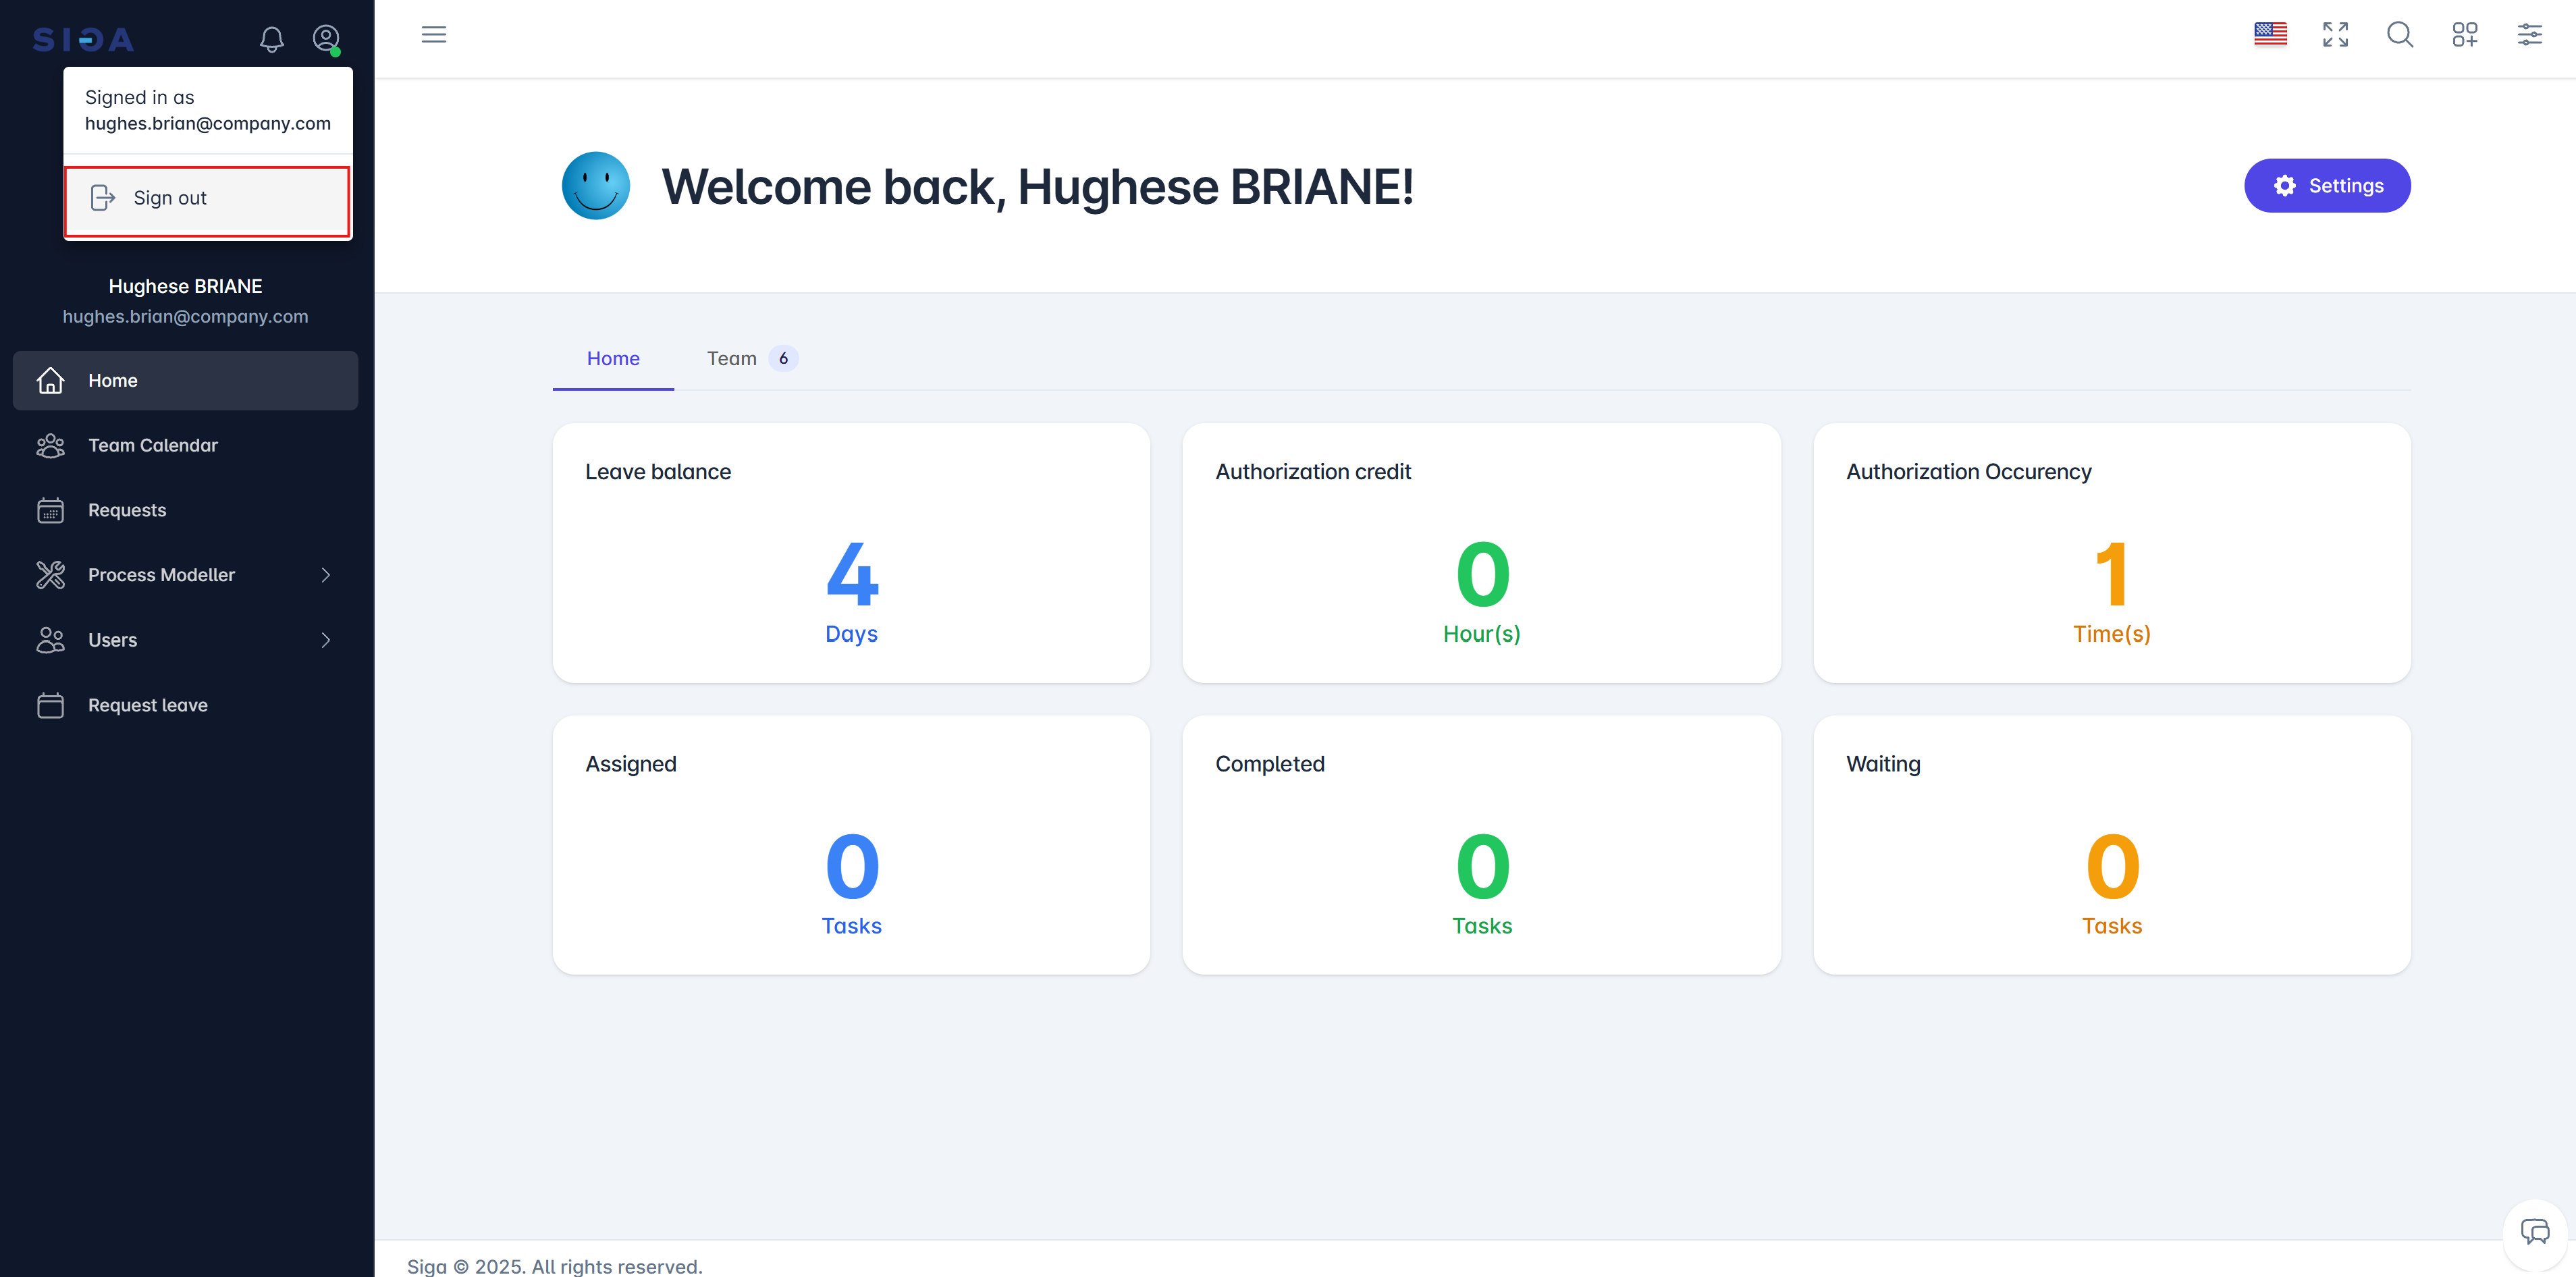
\includegraphics[width=16cm]{images/realisation/decon.png}
     \caption{Interface du cas d'utilisation <<Se déconnecter>>}
     \label{fig:reallogout}
\end{figure}
\subsection{Gérer les utilisateurs}
La gestion des utilisateurs permet à l’administrateur de consulter,ajouter,modifier, supprimer et consulter les détails des utilisateurs.
\subsubsection{Ajouter un utilisateur}
L'administrateur peut ajouter un nouvel utilisateur à l’application via l’interface dédiée accessible depuis le menu latéral, comme illustré dans la figure \ref{fig:adduser}. Il lui suffit de renseigner les informations demandées telles que le prénom, le nom, l’adresse e-mail, le mot de passe, le rôle ainsi qu’un avatar, puis de cliquer sur Create account pour finaliser l’ajout.
\begin{figure}[H]
     \centering
     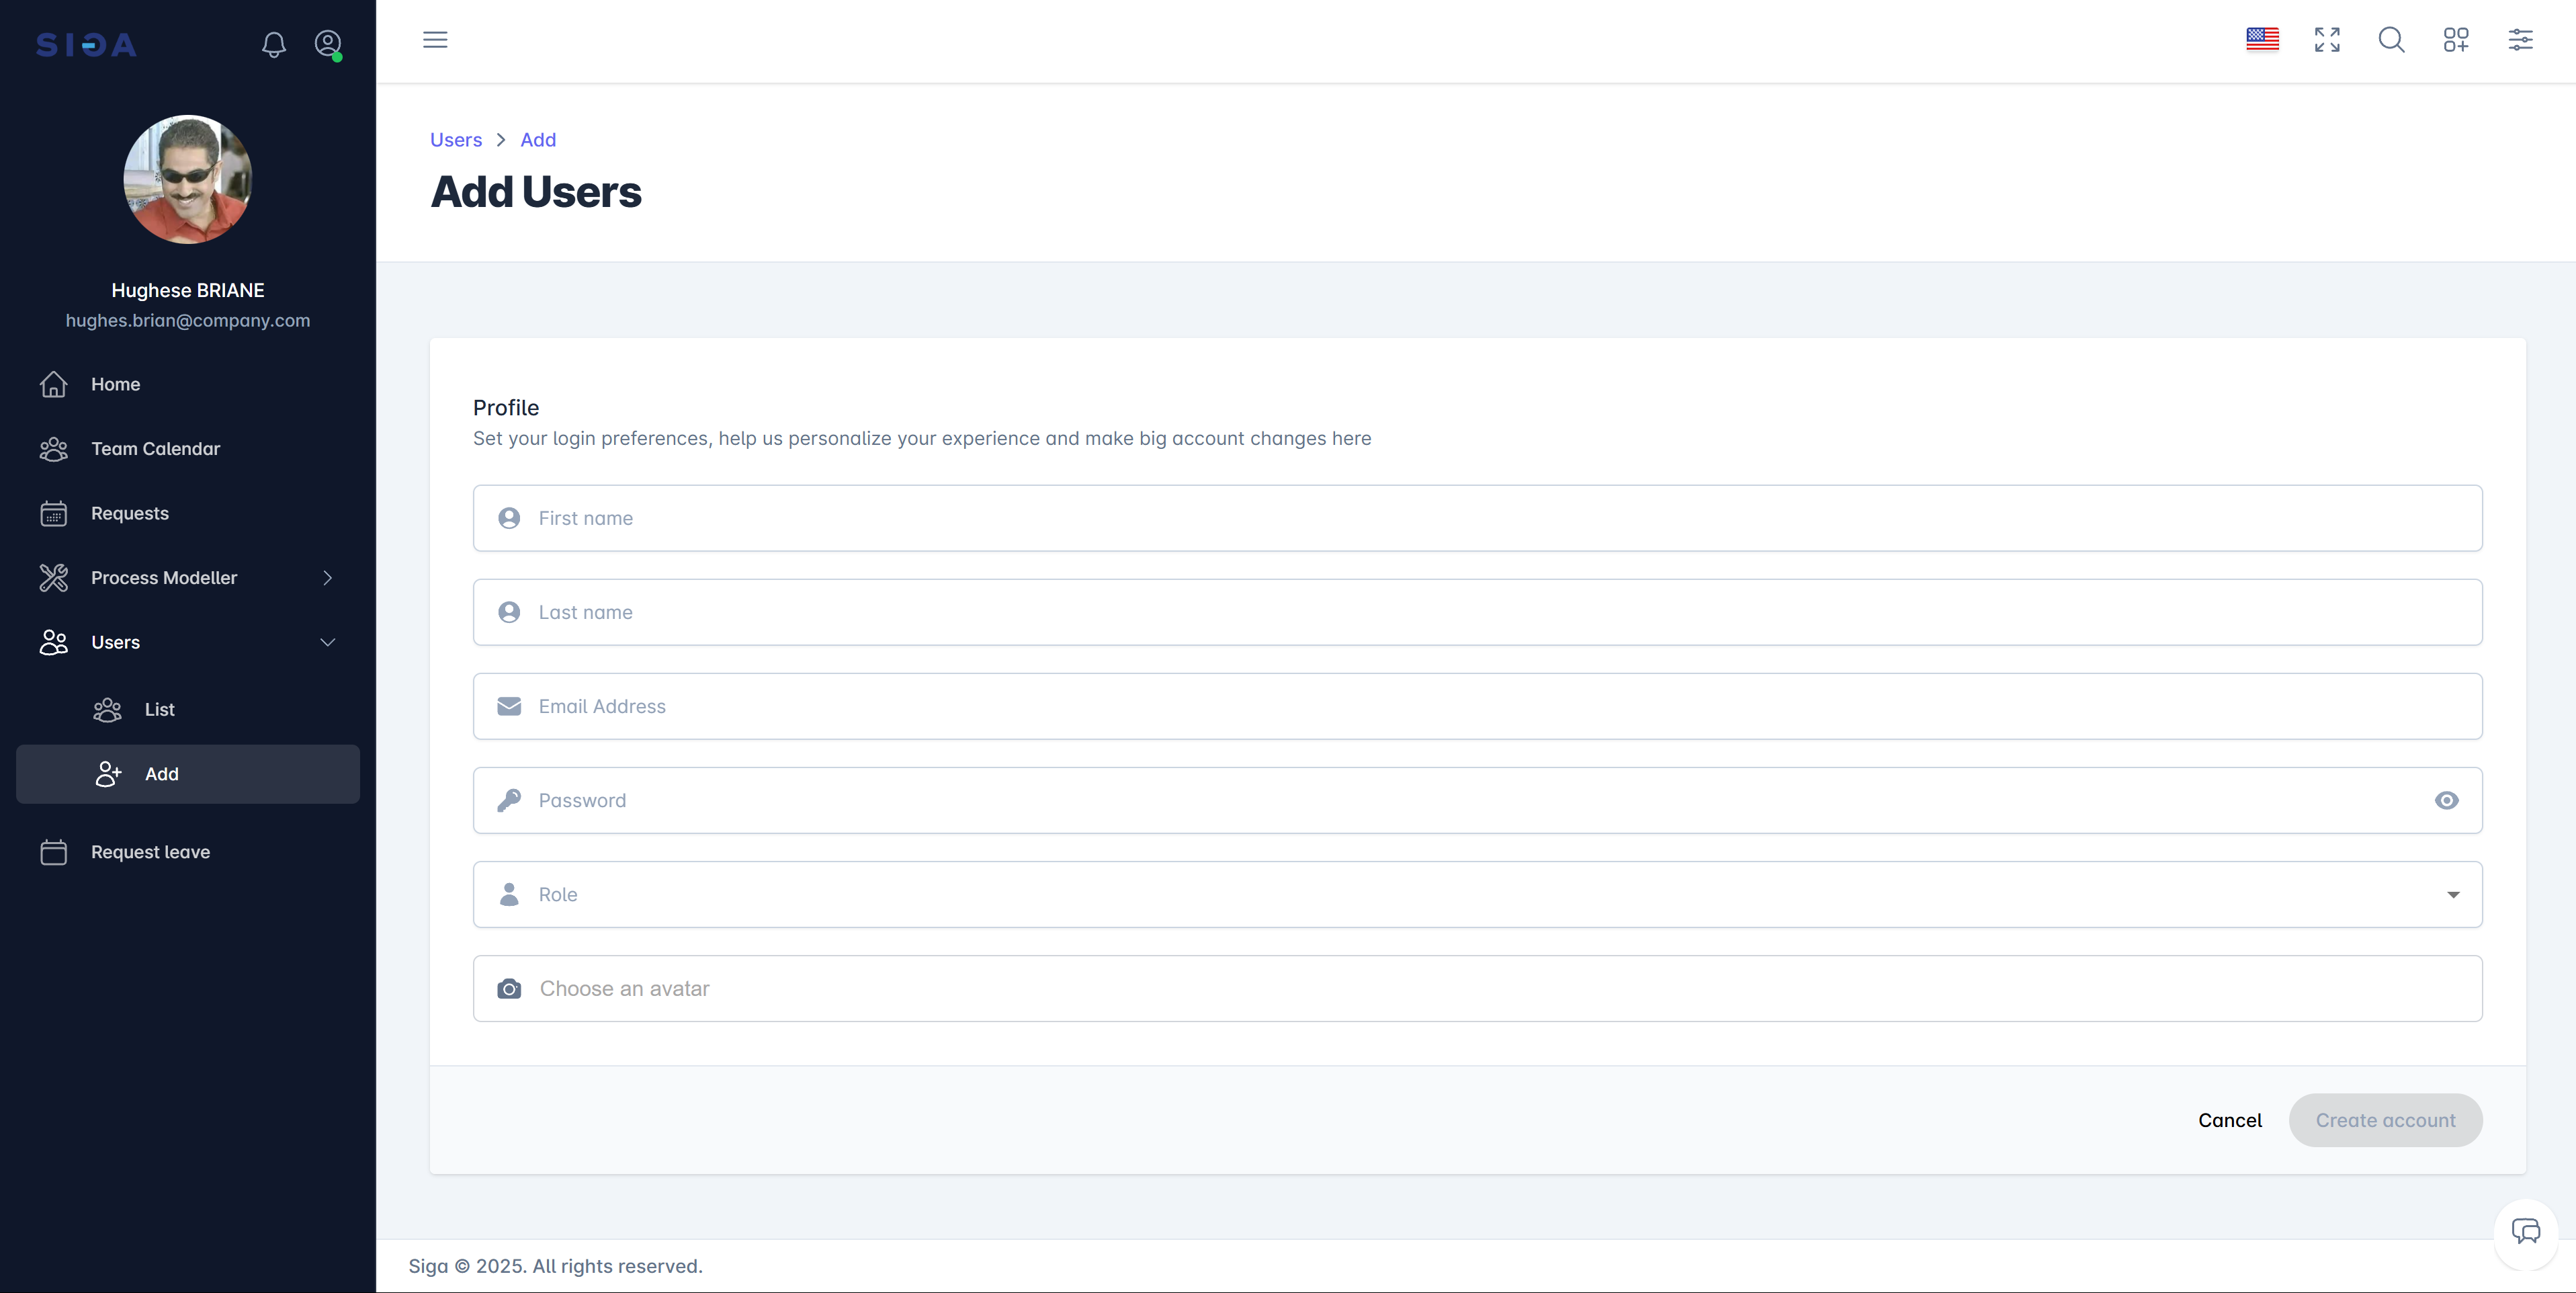
\includegraphics[width=15cm]{images/realisation/addUser.png}
     \caption{Interface du cas d'utilisation <<Ajouter un utilisateur>>}
     \label{fig:adduser}
\end{figure}
\newpage
\subsubsection{Consulter les utilisateurs}
L’administrateur peut consulter la liste des utilisateurs existants via l’onglet Users > List dans le menu latéral, comme le montre la figure \ref{fig:viewusers}. Cette interface permet d’avoir un aperçu global des comptes enregistrés, incluant leurs informations de profil et leur rôle dans le système.
\begin{figure}[H]
     \centering
     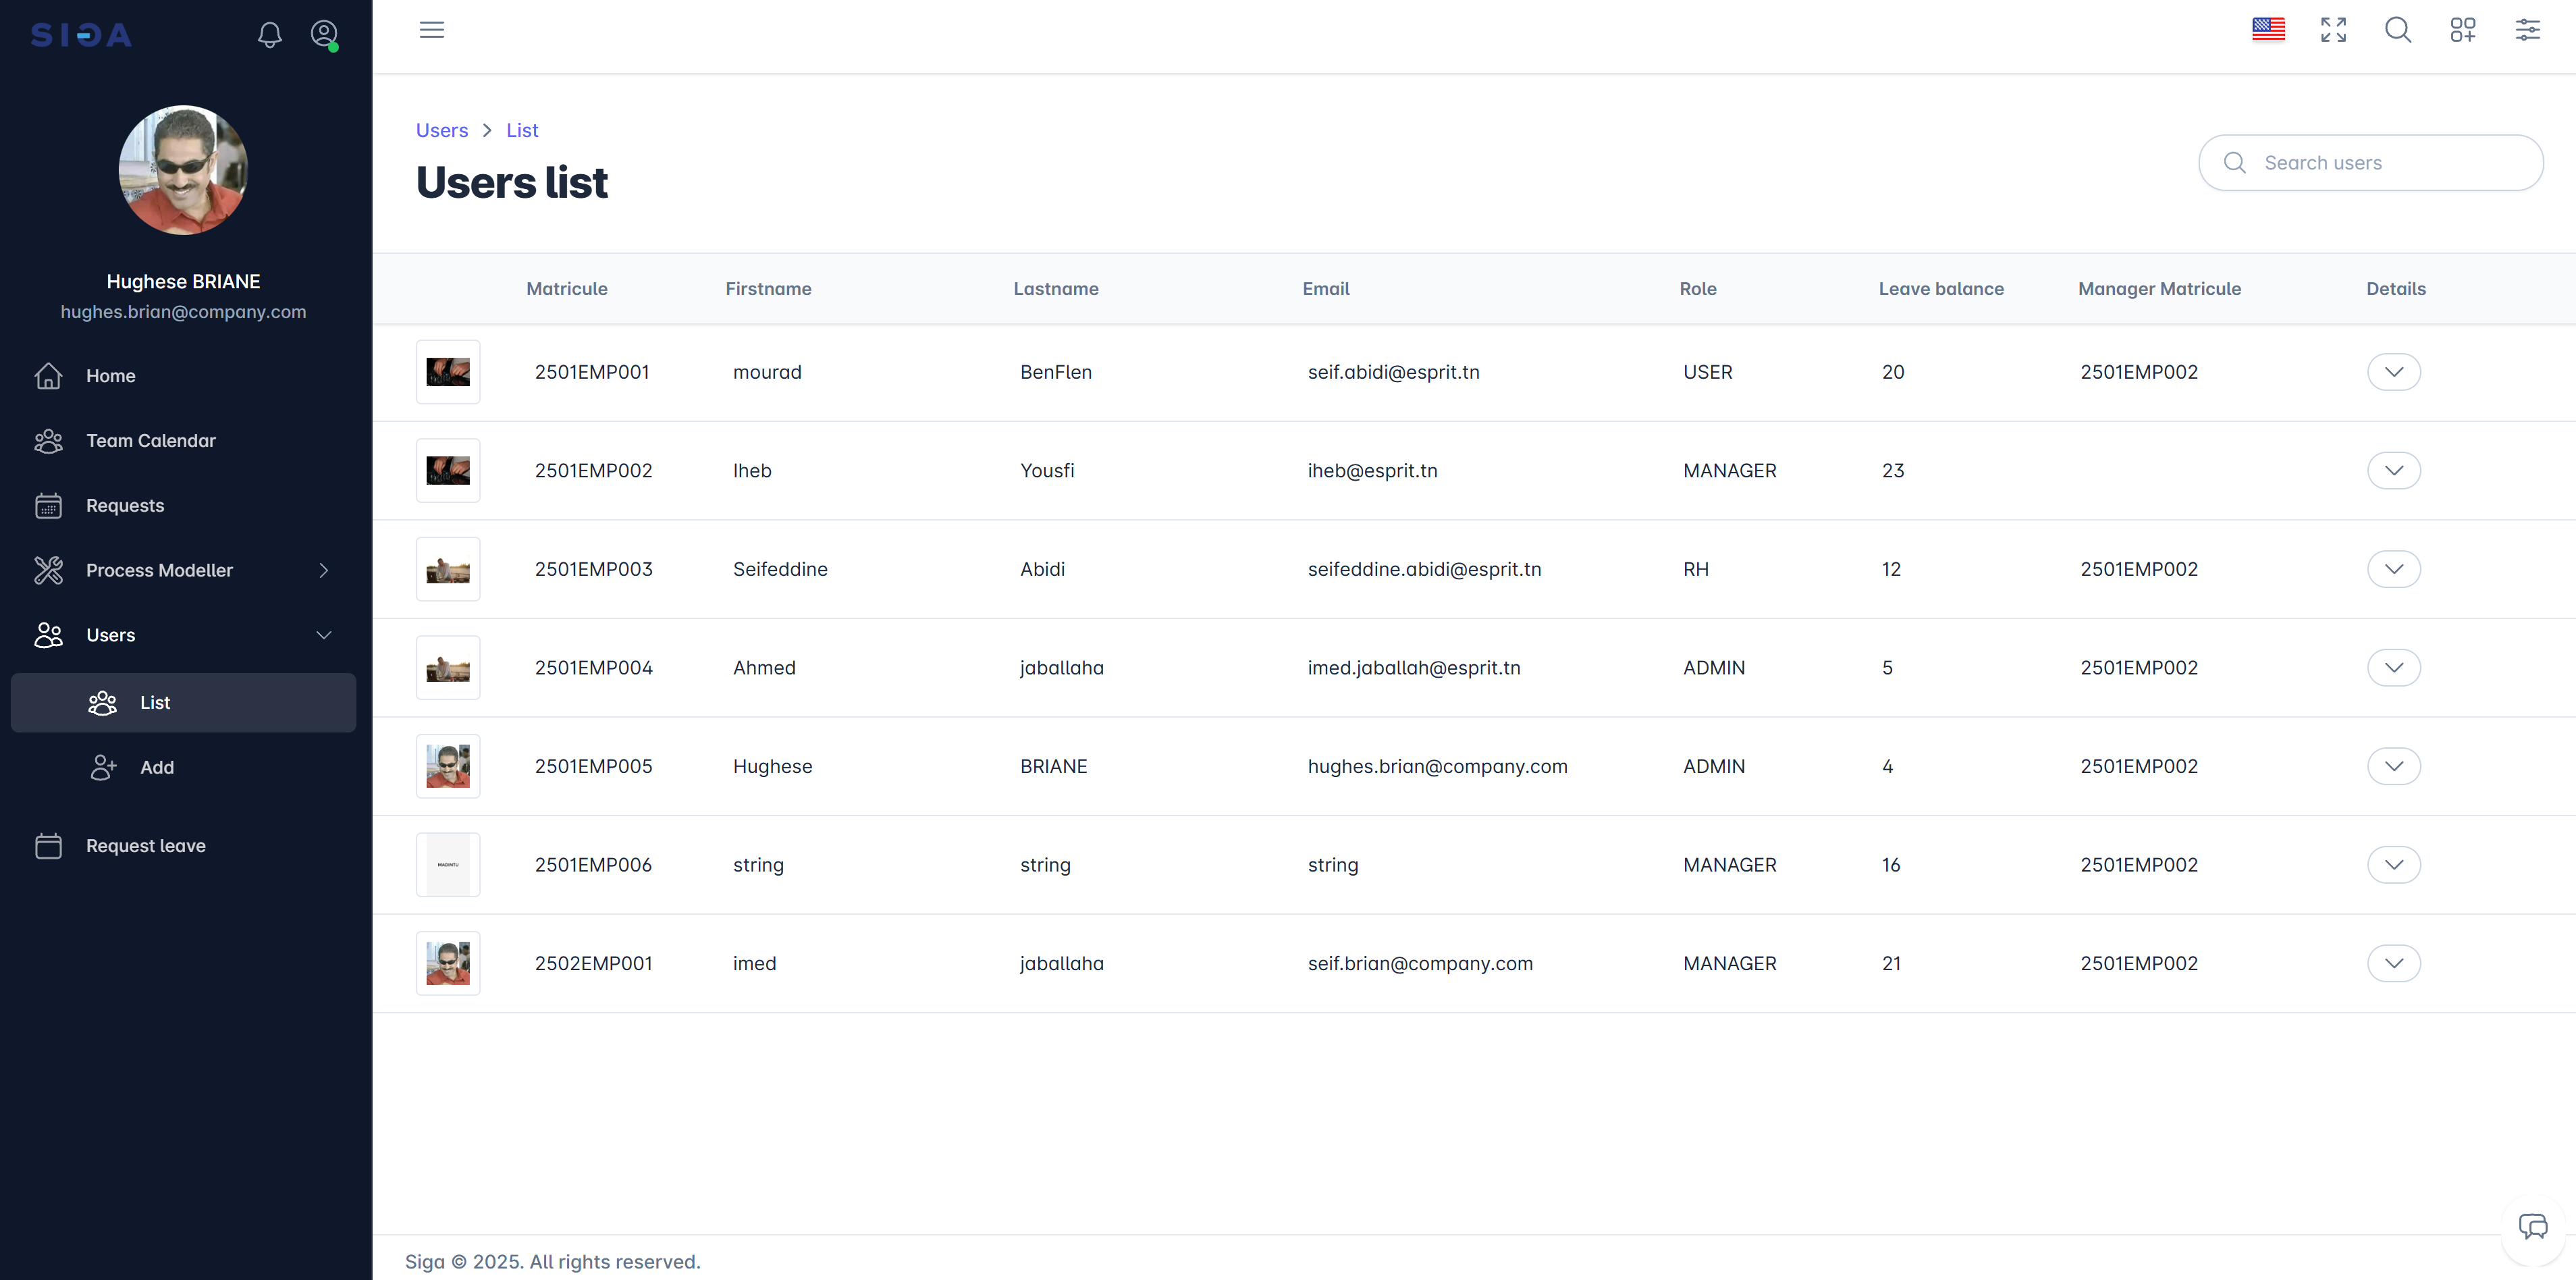
\includegraphics[width=16cm]{images/realisation/vUser.png}
     \caption{Interface du cas d'utilisation <<Consulter les utilisateurs>>}
     \label{fig:viewusers}
\end{figure}
\subsubsection{Consulter les détails d'un utilisateur}
L’administrateur peut consulter les détails d’un compte spécifique en sélectionnant un utilisateur dans la liste, comme illustré dans la figure \ref{fig:userdetails}. Cette action affiche les informations complètes du profil sélectionné.
\begin{figure}[H]
     \centering
     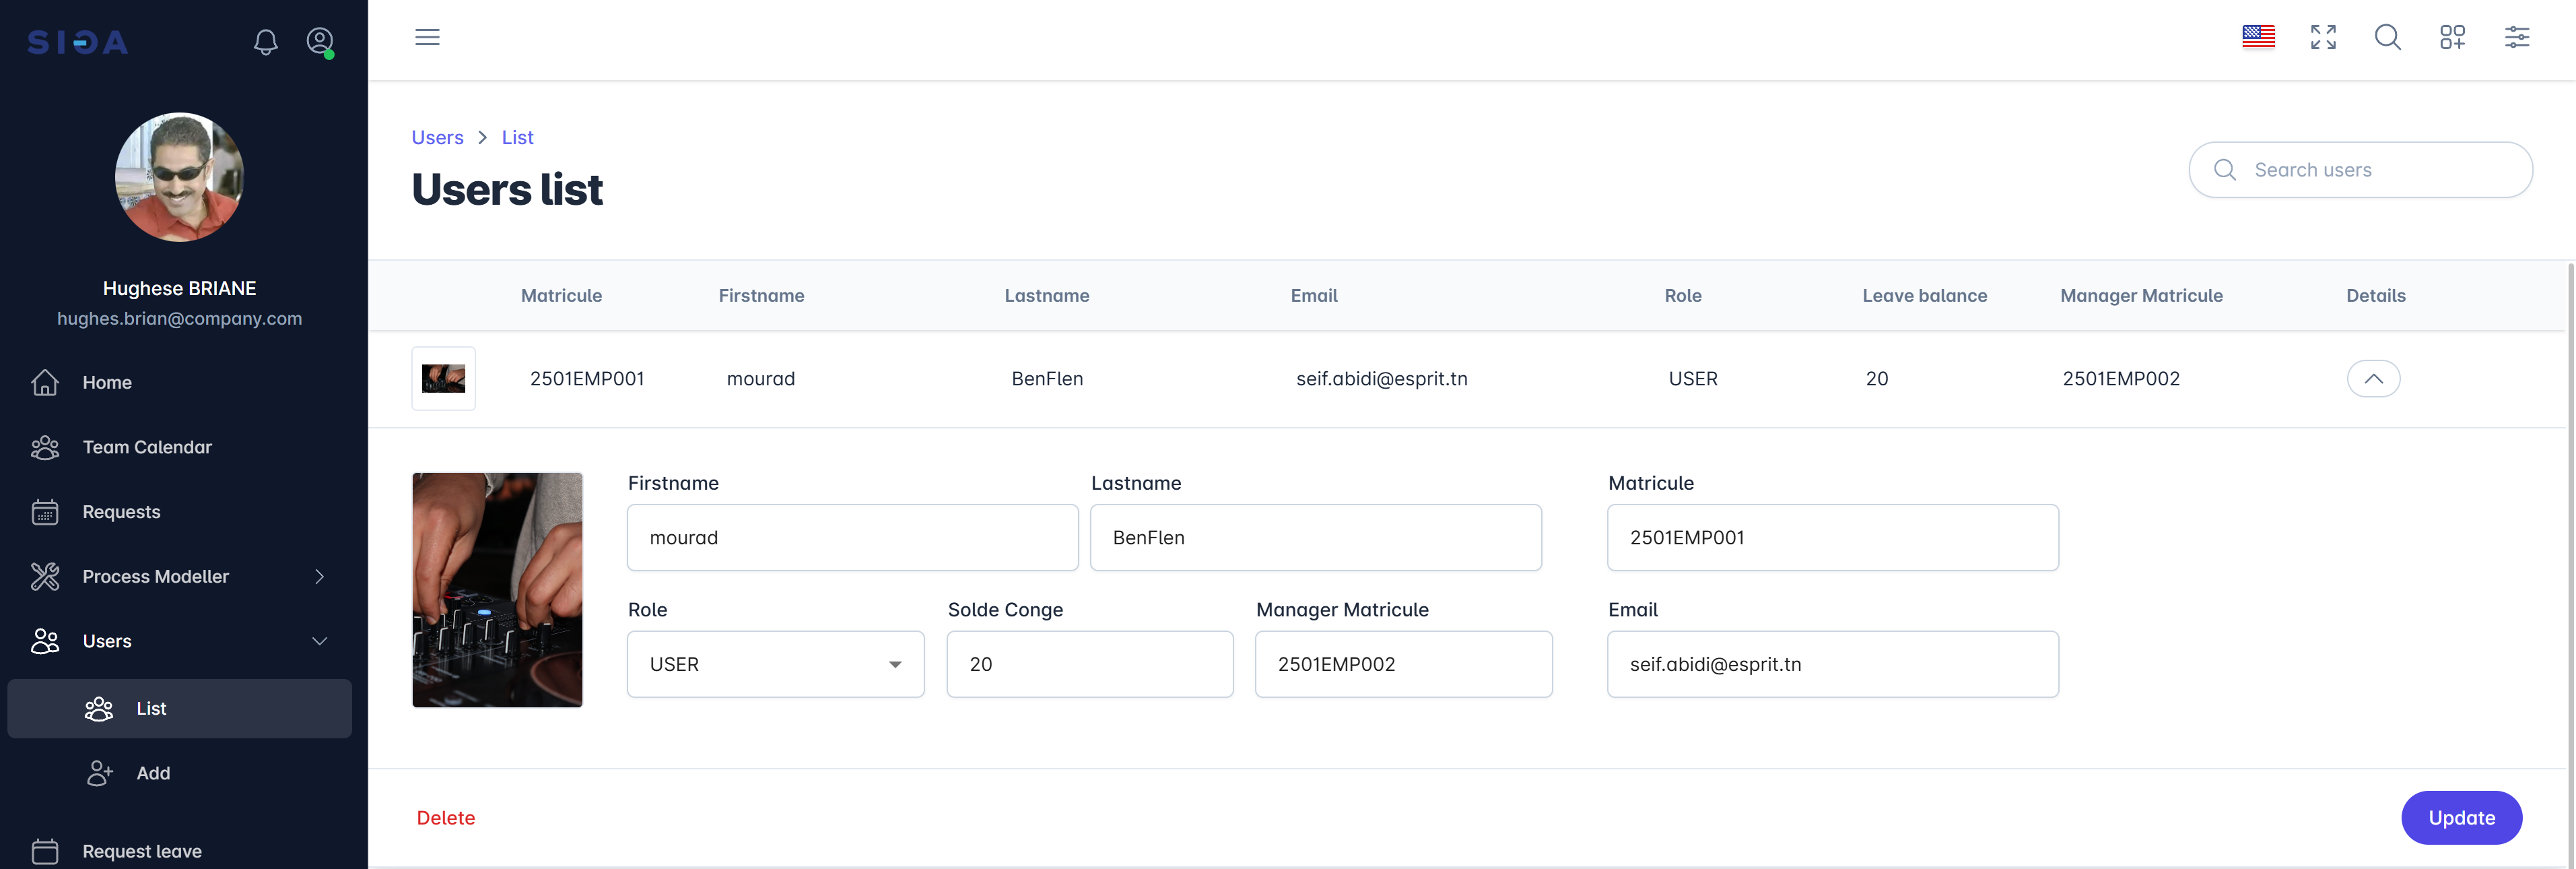
\includegraphics[width=16cm]{images/realisation/dUser.png}
     \caption{Interface du cas d'utilisation <<Consulter les détails d'un utilisateur>>}
     \label{fig:userdetails}
\end{figure}
\newpage
\subsubsection{Modifier un utilisateur}
L’administrateur peut modifier les informations d’un compte existant en accédant à son profil depuis la liste des utilisateurs, comme le montre la figure \ref{fig:edituser}. Une fois les champs mis à jour (nom, e-mail, rôle, etc.), il peut enregistrer les modifications pour qu’elles soient prises en compte immédiatement.
\begin{figure}[H]
     \centering
     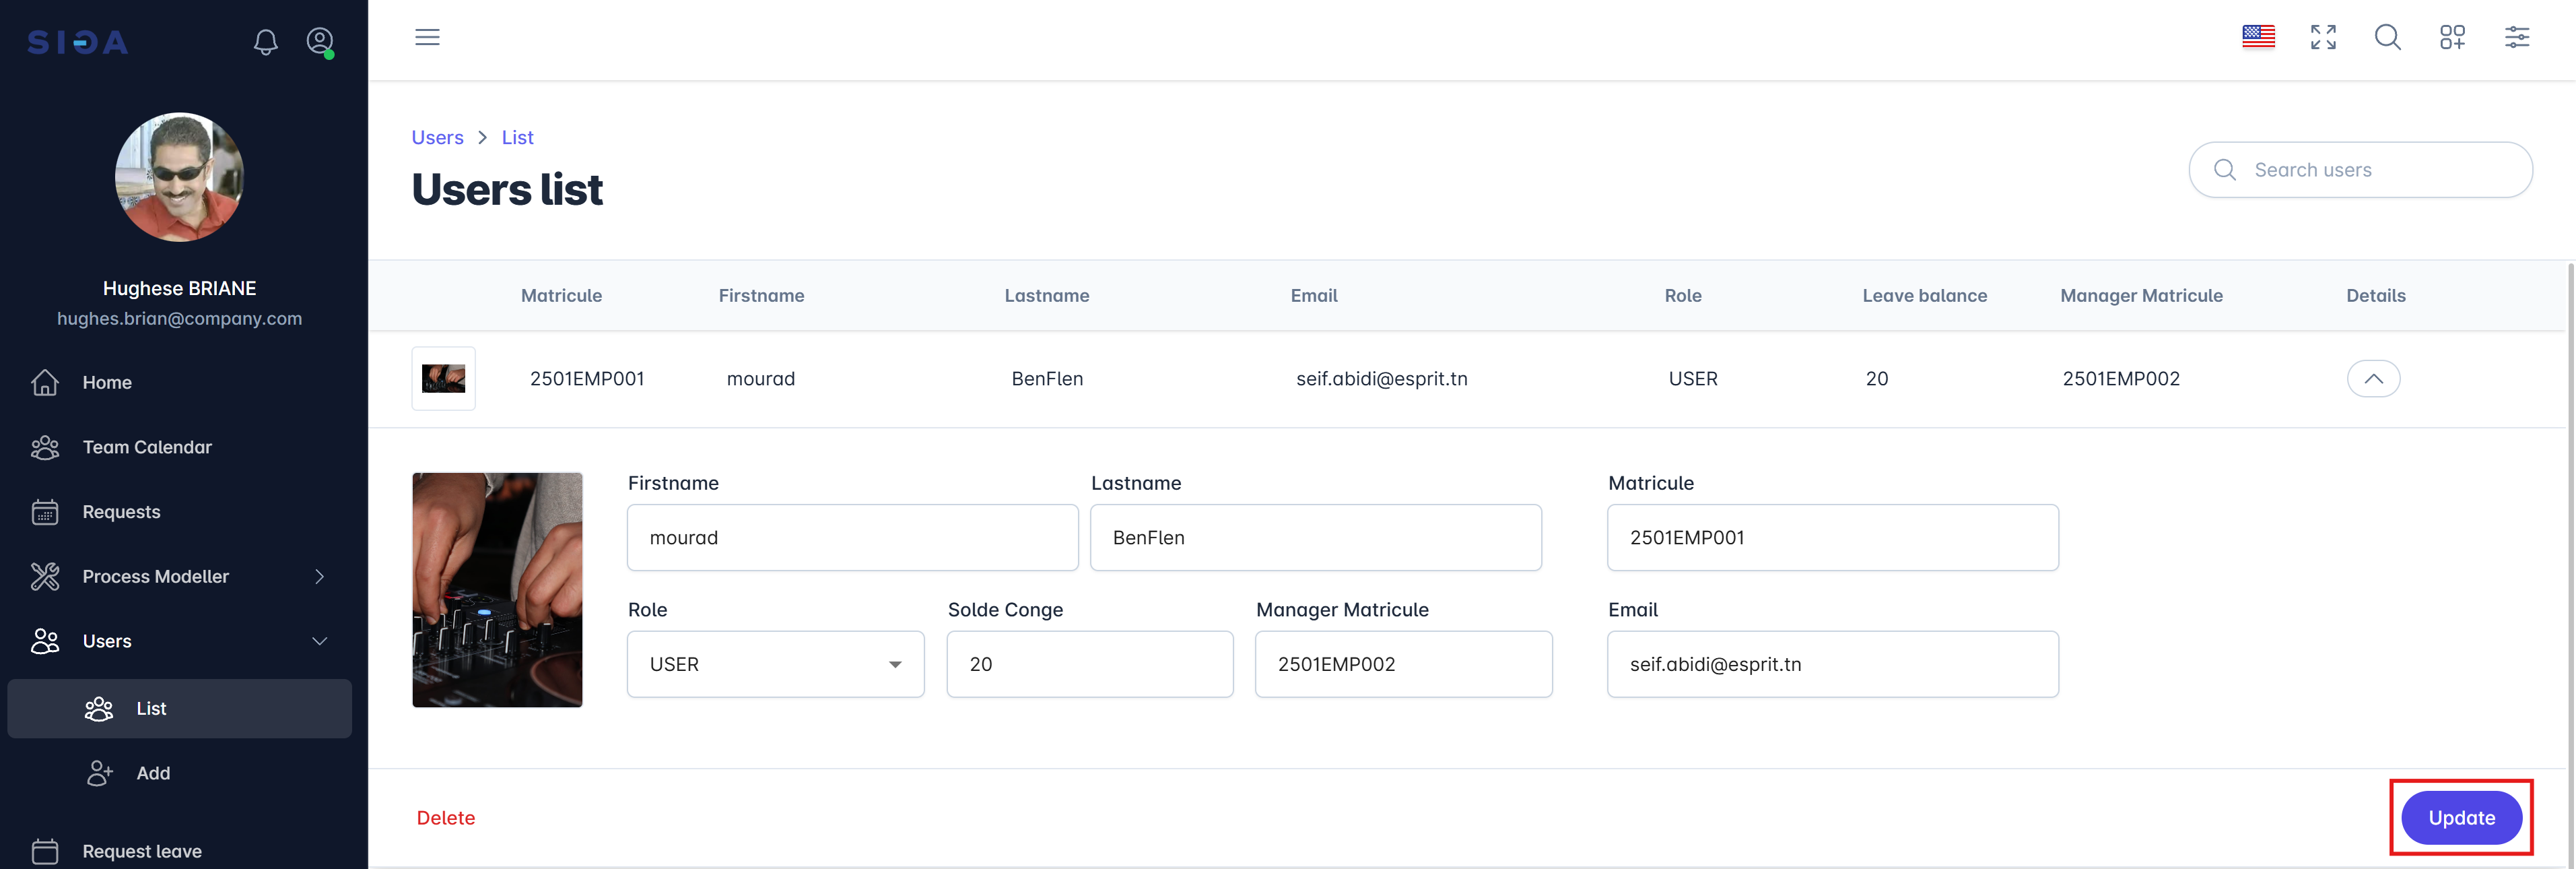
\includegraphics[width=16cm]{images/realisation/mUser.png}
     \caption{Interface du cas d'utilisation <<Modifier un utilisateur>>}
     \label{fig:edituser}
\end{figure}
\subsubsection{Supprimer un utilisateur}
L’administrateur peut supprimer un compte utilisateur en accédant à la liste des utilisateurs et en sélectionnant l’option de suppression associée, comme illustré dans la figure \ref{fig:deleteuser}. Une confirmation est demandée avant la suppression définitive afin d’éviter toute action involontaire.
\begin{figure}[H]
     \centering
     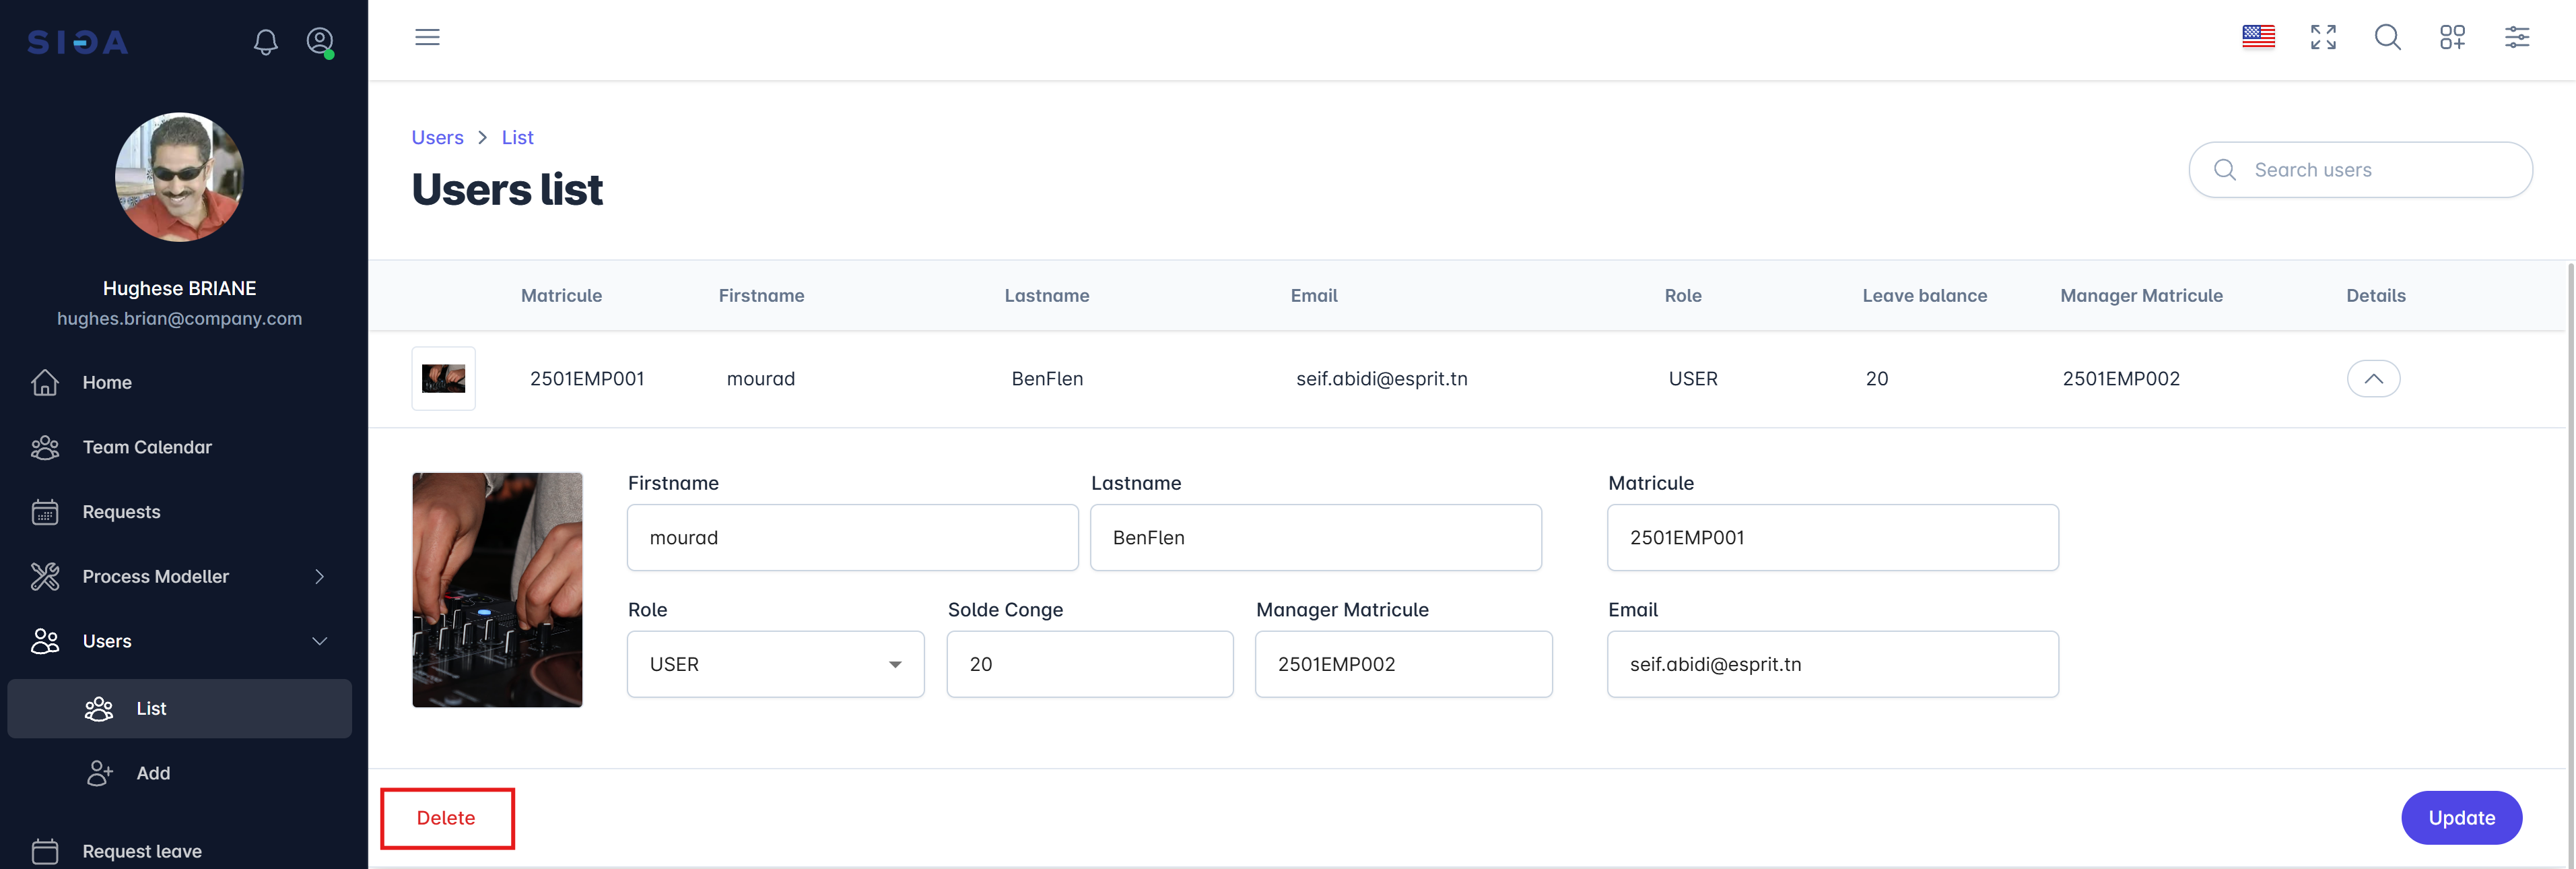
\includegraphics[width=16cm]{images/realisation/sUser.png}
     \caption{Interface du cas d'utilisation <<Supprimer un utilisateur>>}
     \label{fig:deleteuser}
\end{figure}
\newpage
\subsubsection{Intégrer Camunda}
Afin d’intégrer le moteur de workflow Camunda au projet, l’utilisateur doit ajouter les dépendances nécessaires dans le fichier pom.xml, comme illustré dans la figure \ref{fig:camunda-dependencies}. Ces dépendances permettent d’activer le moteur BPM, l’interface web de gestion, ainsi que l’accès aux API REST de Camunda.
\begin{figure}[H]
     \centering
     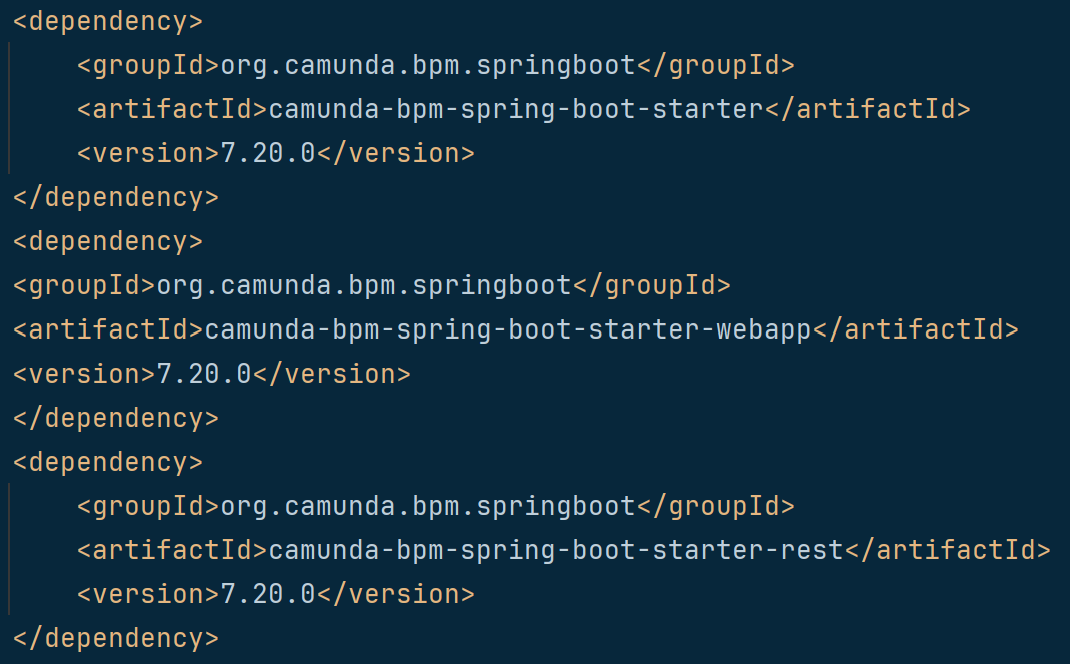
\includegraphics[width=11cm]{images/realisation/cam.png}
     \caption{Interface d'intégration de Camunda}
     \label{fig:camunda-dependencies}
\end{figure}
\subsubsection{Configurer Camunda}
Après avoir ajouté les dépendances nécessaires, l’utilisateur doit configurer Camunda dans le fichier application.properties, comme montré dans la figure \ref{fig:camunda-config}. Cette configuration permet de personnaliser des paramètres essentiels tels que l’authentification, l’accès à l’interface web ou encore le comportement du moteur de workflow au démarrage.
\begin{figure}[H]
     \centering
     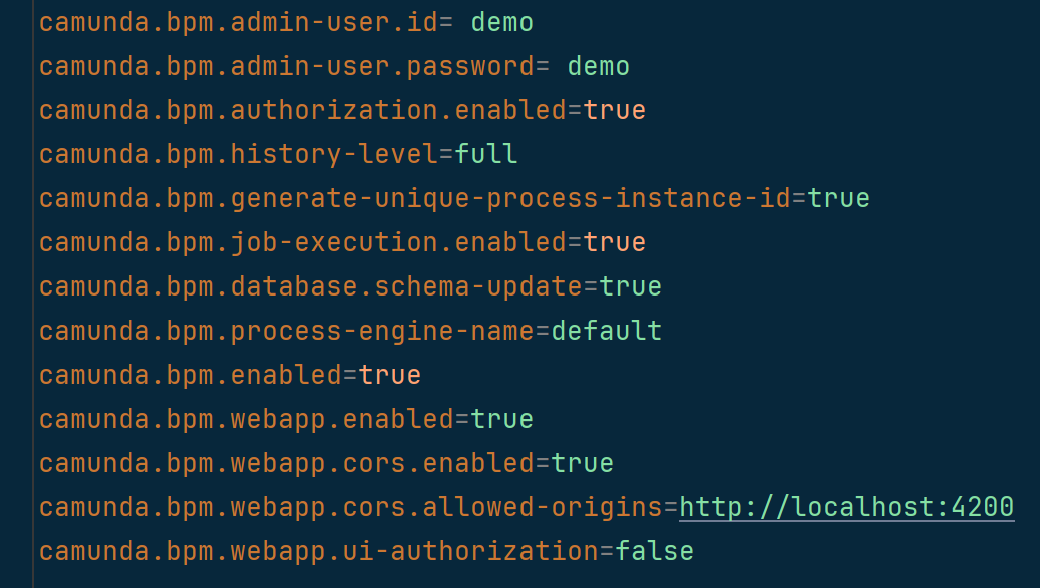
\includegraphics[width=11cm]{images/realisation/camm.png}
     \caption{Interface de configuration de Camunda}
     \label{fig:camunda-config}
\end{figure}
\newpage
\subsubsection{Interface de Camunda}
Une fois l’application démarrée, l’utilisateur ayant les droits appropriés peut accéder à l’interface Cockpit de Camunda, comme illustré dans la figure \ref{fig:camunda-cockpit}. Cette interface web permet de surveiller les processus en cours d’exécution, d’examiner les incidents, et d’analyser les performances du moteur BPMN en temps réel.
\begin{figure}[H]
     \centering
     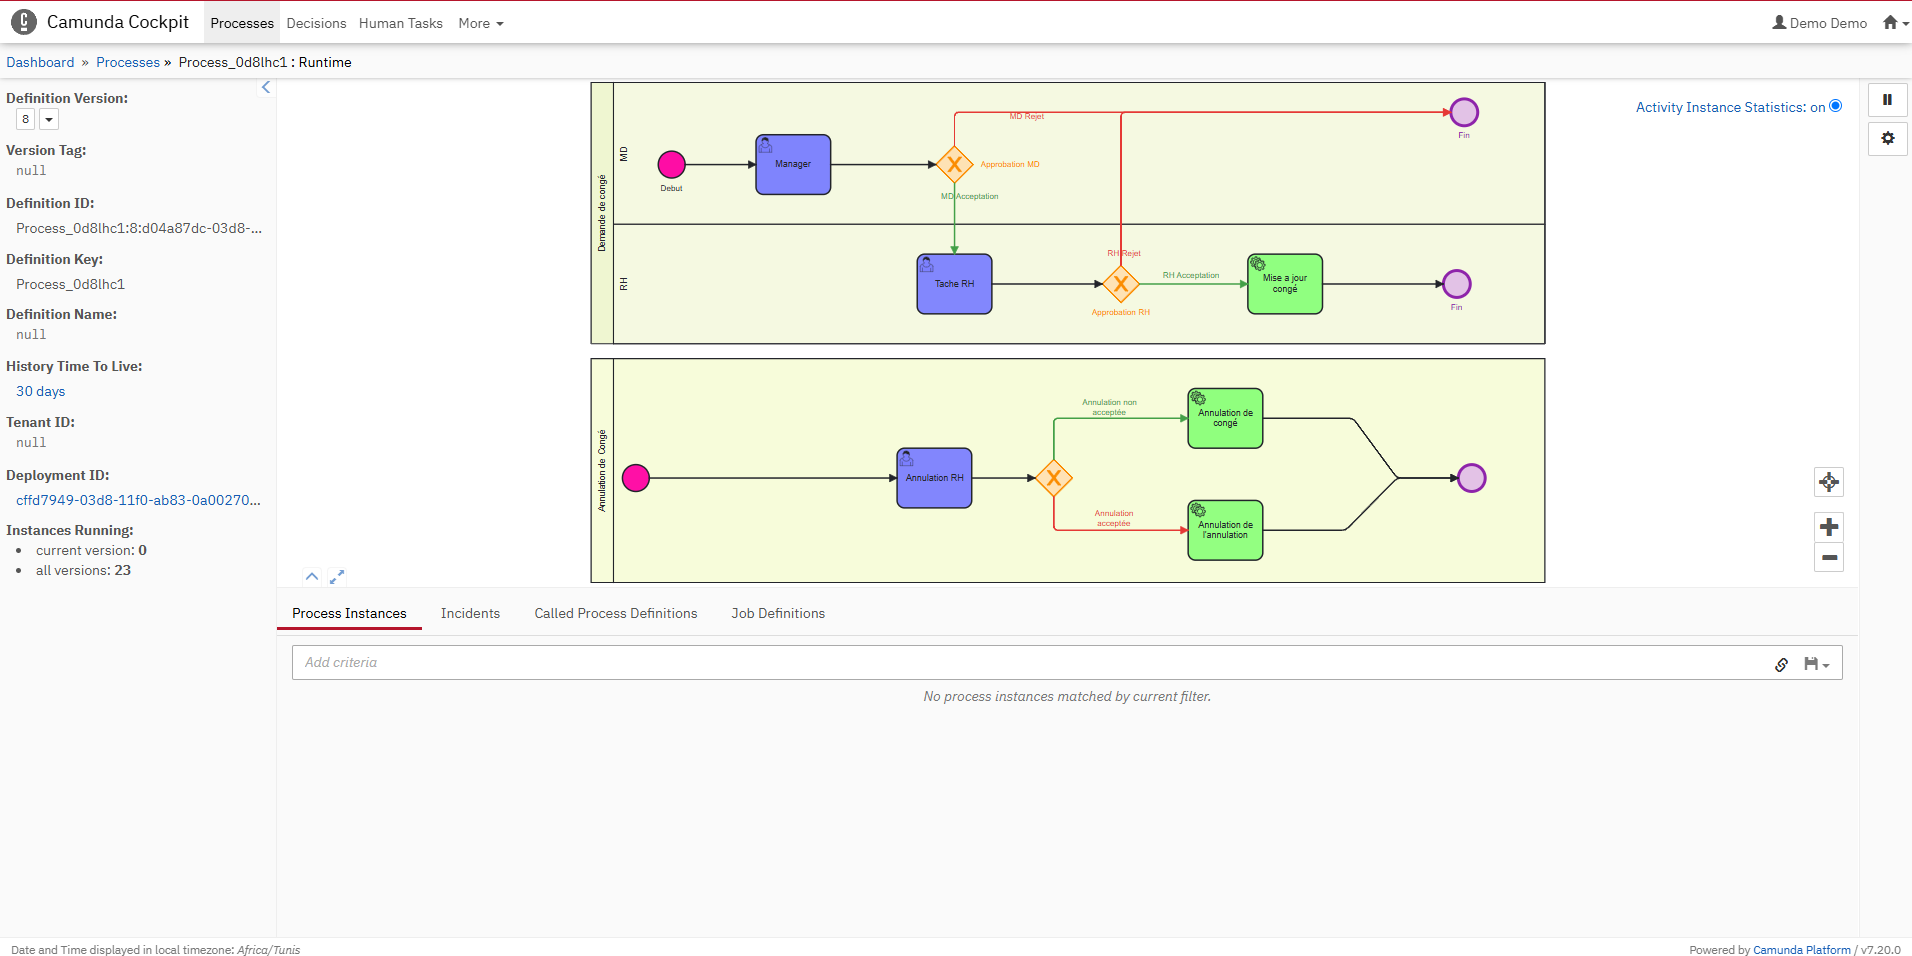
\includegraphics[width=15cm]{images/realisation/pit.png}
     \caption{Interface cockpit de Camunda}
     \label{fig:camunda-cockpit}
\end{figure}
\section{Conclusion}

Le premier sprint du projet a permis de poser des bases solides pour la gestion des accès et l'administration de la plateforme. En implémentant les fonctionnalités clés d'authentification, de déconnexion, de gestion des utilisateurs et d'intégration de Camunda, nous avons établi une infrastructure robuste et sécurisée, essentielle pour les sprints futurs. Les cas d'utilisation ont été soigneusement raffinés, conçus et réalisés, avec des interfaces utilisateur intuitives et des mécanismes techniques fiables, tels que l'utilisation des tokens JWT pour l'authentification, renforcés par les adresses IP des clients et les informations du client-agent (navigateur) pour ajouter une couche supplémentaire de sécurité. L'intégration du moteur de workflow Camunda a également permis de structurer et gérer les processus de manière fluide et évolutive.\\

Cette étape a non seulement répondu aux besoins fonctionnels prioritaires, mais a également renforcé la qualité, la sécurité et la fiabilité du système grâce à des pratiques de développement rigoureuses. Les fondations établies dans ce sprint garantiront une évolutivité et une maintenabilité optimales pour les prochaines itérations du projet.







 


 


 


\clearpage

\chapter{Sprint 2 : Gestion des demandes}
\section{Introduction}
Après avoir établi les fondations d'accès et d'administration dans le Sprint 1, le Sprint 2 se concentre sur la gestion des demandes au sein de la plateforme. Ce chapitre détaille les fonctionnalités prévues pour permettre aux utilisateurs, managers et RH de gérer efficacement les demandes et congés, tout en offrant des outils pour la consultation et le traitement de ces demandes. Nous aborderons les besoins, la conception et les étapes de réalisation de ce sprint.
\section{Backlog du Sprint 2}
\begin{table}[!ht]
\begin{adjustwidth}{-2.5cm}{-2.5cm}
\centering
\caption{Backlog du Sprint 2}
\label{tab:backlog_sprint2}
\begin{tabular}{ | m{5cm} | m{1cm} | m{5.5cm} | }
\hline
\cellcolor[rgb]{0.832,0.832,0.832}Cas d'utilisation & \cellcolor[rgb]{0.832,0.832,0.832}Priorité & \cellcolor[rgb]{0.832,0.832,0.832}Tâche \\
\hline
Gérer son profil & 2 & Modifier ses informations (nom, prénom, e-mail, etc.) \\
\hline
Réinitialiser son mot de passe & 2 & Utilisateur réinitialise via un lien sécurisé \\
\hline
Soumettre une demande & 2 & Utilisateurs, Managers, RH soumettent des demandes \\
\hline
Consulter ses demandes & 2 & Utilisateurs, Managers, RH consultent l’historique \\
\hline
Consulter ses congés & 2 & Utilisateurs, Managers, RH consultent congés, solde \\
\hline
Traiter une demande & 2 & Managers, RH valident ou rejettent les demandes \\
\hline
\end{tabular}
\end{adjustwidth}
\end{table}
\section{Rafinnement de cas d'utilisation }
Cette partie consiste à analyser et spécifier les besoins de ce deuxième sprint à travers l’identification des acteurs et le raffinement des cas d’utilisations.
\subsection{Identification des acteurs du deuxième sprint}
Les acteurs de ce sprint sont : \\
\textbf{Utilisateur} : Soumet des demandes (congés, absences) et consulte ses propres demandes et congés. \\
\textbf{Manager} : Soumet, consulte et traite les demandes (validation/rejet). \\
\textbf{RH (Ressources Humaines)} : Soumet, consulte et traite les demandes, gère les congés.
\subsection{Raffinement du Cas d'Utilisation <<Gérer son Profil>>}
La figure~\ref{fig:usecaseGP} illustre le diagramme de cas d'utilisation « Gérer le profil ».
\begin{figure}[h]
     \centering
     \fbox{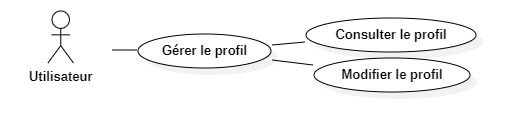
\includegraphics[width=11cm]{images/UMPRFL.jpg}}
     \caption{Diagramme du cas d'utilisation <<Gérer le profil>>}
     \label{fig:usecaseGP}
\end{figure}\\
\begin{table}[!ht]
\centering
\caption{Description textuelle du Cas d’utilisation «Consulter le Profil»}
\label{tab:view_profile}
\renewcommand{\arraystretch}{1.2}
\begin{tabular}{|p{4.2cm}|p{11cm}|}
\hline
\textbf{Cas d'utilisation} & Consulter le Profil \\
\hline
\textbf{Acteur} & Utilisateur, Manager, RH\\
\hline
\textbf{Pré-conditions} & Système en marche. \newline Utilisateur authentifié. \\
\hline
\textbf{Post-conditions} & Profil consulté. \\
\hline
\textbf{Scénario de Base} & 
1. Le système affiche l'interface du profil de l'utilisateur. \newline
2. L'utilisateur consulte la liste des informations de son profil. \\
\hline
\textbf{Exceptions} & 
Échec de consultation (problème dans l’API GET, problème dans la base de données). \\
\hline
\end{tabular}
\end{table}
Le tableau~\ref{tab:view_profile} illustre la description textuelle du cas d’utilisation « Consulter le Profil ».
\newpage
Le tableau~\ref{tab:edit_profile} illustre la description textuelle du cas d’utilisation « Modifier le Profil ».
\begin{table}[!ht]
\centering
\caption{Description textuelle du Cas d’utilisation «Modifier le Profil»}
\label{tab:edit_profile}
\renewcommand{\arraystretch}{1.2}
\begin{tabular}{|p{4.2cm}|p{11cm}|}
\hline
\textbf{Cas d'utilisation} & Modifier le Profil \\
\hline
\textbf{Acteur} & Utilisateur \\
\hline
\textbf{Pré-conditions} & Système en marche. \newline Utilisateur authentifié. \\
\hline
\textbf{Post-conditions} & Profil modifié. \\
\hline
\textbf{Scénario de Base} & 
1. Le système affiche l'interface du profil de l'utilisateur. \newline
2. L'utilisateur modifie les informations choisies. \newline
3. L'utilisateur clique sur le bouton « Modifier ». \newline
4. Le système modifie ces informations. \newline
5. Le système affiche un message de succès de modification. \\
\hline
\textbf{Exceptions} & 
Échec de modification (problème dans l’API PUT, problème dans la base de données). \\
\hline
\end{tabular}
\end{table}
\subsection{Raffinement du Cas d'Utilisation <<Réinitialiser son Mot de Passe>>}
La figure~\ref{fig:usecase_reset_password} illustre le diagramme de cas d'utilisation « Réinitialiser son Mot de Passe ».
\begin{figure}[h]
     \centering
     \fbox{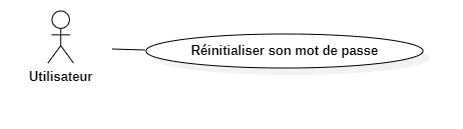
\includegraphics[width=11cm]{images/resetP.jpg}}
     \caption{Diagramme du cas d'utilisation <<Réinitialiser son Mot de Passe>>}
     \label{fig:usecase_reset_password}
\end{figure}\\
Le tableau~\ref{tab:reset_password} illustre la description textuelle du cas d’utilisation « Réinitialiser son Mot de Passe ».
\newpage
\begin{table}[!ht]
\centering
\caption{Description textuelle du Cas d’utilisation «Réinitialiser son Mot de Passe»}
\label{tab:reset_password}
\renewcommand{\arraystretch}{1.2}
\begin{tabular}{|p{4.2cm}|p{11cm}|}
\hline
\textbf{Cas d'utilisation} & Réinitialiser son Mot de Passe \\
\hline
\textbf{Acteur} & Utilisateur \\
\hline
\textbf{Pré-conditions} & Système en marche. \newline Utilisateur inscrit avec un e-mail valide. \\
\hline
\textbf{Post-conditions} & Mot de passe réinitialisé. \\
\hline
\textbf{Scénario de Base} & 
1. L’utilisateur clique sur « Mot de passe oublié » sur la page de connexion. \newline
2. Il entre son adresse e-mail et soumet la demande. \newline
3. Le système envoie un lien sécurisé à l’e-mail de l’utilisateur. \newline
4. L’utilisateur clique sur le lien et entre un nouveau mot de passe. \newline
5. Le système enregistre le nouveau mot de passe et affiche un message de succès. \\
\hline
\textbf{Exceptions} & 
Échec de réinitialisation (e-mail invalide, lien expiré, problème API). \\
\hline
\end{tabular}
\end{table}

\subsection{Raffinement du Cas d'Utilisation <<Soumettre une Demande>>}
La figure~\ref{fig:usecase_submit_request} illustre le diagramme de cas d'utilisation « Soumettre une Demande ».
\begin{figure}[h]
     \centering
     \fbox{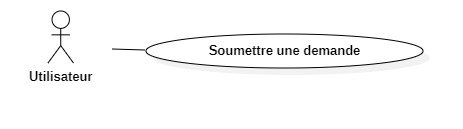
\includegraphics[width=11cm]{images/SMD.jpg}}
     \caption{Diagramme du cas d'utilisation <<Soumettre une Demande>>}
     \label{fig:usecase_submit_request}
\end{figure}\\
Le tableau~\ref{tab:submit_request} illustre la description textuelle du cas d’utilisation « Soumettre une Demande ».
\newpage
\begin{table}[!ht]
\centering
\caption{Description textuelle du Cas d’utilisation «Soumettre une Demande»}
\label{tab:submit_request}
\renewcommand{\arraystretch}{1.2}
\begin{tabular}{|p{4.2cm}|p{11cm}|}
\hline
\textbf{Cas d'utilisation} & Soumettre une Demande \\
\hline
\textbf{Acteur} & Utilisateur, Manager, RH \\
\hline
\textbf{Pré-conditions} & Système en marche. \newline Acteur authentifié. \\
\hline
\textbf{Post-conditions} & Demande enregistrée et parties concernées notifiées. \\
\hline
\textbf{Scénario de Base} & 
1. L’acteur accède au formulaire de soumission. \newline
2. L’acteur sélectionne le type de demande : \newline
   \quad a. \textit{Demande de Congé} : Formulaire avec les champs (dates de début et fin, type de congé, motif). \newline
   \quad b. \textit{Demande d’Autorisation} : Formulaire avec les champs (date, durée). \newline
3. Il remplit les détails selon le formulaire correspondant. \newline
4. Il soumet la demande. \newline
5. Le système enregistre la demande et notifie les parties concernées. \\
\hline
\textbf{Exceptions} & 
Échec de soumission (données invalides, erreur API). \\
\hline
\end{tabular}
\end{table}
\subsection{Raffinement du Cas d'Utilisation <<Consulter ses Demandes>>}
La figure~\ref{fig:usecase_view_requests} illustre le diagramme de cas d'utilisation « Consulter ses Demandes ».
\begin{figure}[h]
     \centering
     \fbox{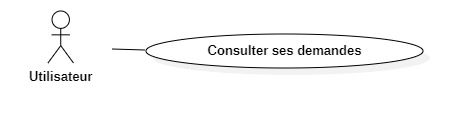
\includegraphics[width=11cm]{images/CSD.jpg}}
     \caption{Diagramme du cas d'utilisation <<Consulter ses Demandes>>}
     \label{fig:usecase_view_requests}
\end{figure}\\
Le tableau~\ref{tab:view_requests} illustre la description textuelle du cas d’utilisation « Consulter ses Demandes ».
\newpage
\begin{table}[!ht]
\centering
\caption{Description textuelle du Cas d’utilisation «Consulter ses Demandes»}
\label{tab:view_requests}
\renewcommand{\arraystretch}{1.2}
\begin{tabular}{|p{4.2cm}|p{11cm}|}
\hline
\textbf{Cas d'utilisation} & Consulter ses Demandes \\
\hline
\textbf{Acteur} & Utilisateur, Manager, RH \\
\hline
\textbf{Pré-conditions} & Système en marche. \newline Acteur authentifié. \\
\hline
\textbf{Post-conditions} & Historique des demandes affiché. \\
\hline
\textbf{Scénario de Base} & 
1. L’acteur accède à la section « Mes Demandes ». \newline
2. Le système affiche la liste des demandes avec leur statut. \\
\hline
\textbf{Exceptions} & 
Échec de consultation (erreur API). \\
\hline
\end{tabular}
\end{table}
\subsection{Raffinement du Cas d'Utilisation <<Consulter ses Congés>>}
La figure~\ref{fig:usecase_view_leaves} illustre le diagramme de cas d'utilisation « Consulter ses Congés ».
\begin{figure}[h]
     \centering
     \fbox{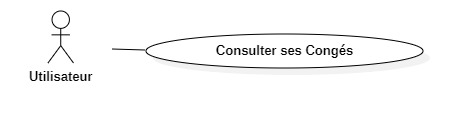
\includegraphics[width=11cm]{images/CSC.jpg}}
     \caption{Diagramme du cas d'utilisation <<Consulter ses Congés>>}
     \label{fig:usecase_view_leaves}
\end{figure}\\
Le tableau~\ref{tab:view_leaves} illustre la description textuelle du cas d’utilisation « Consulter ses Congés ».
\begin{table}[!ht]
\centering
\caption{Description textuelle du Cas d’utilisation «Consulter ses Congés»}
\label{tab:view_leaves}
\renewcommand{\arraystretch}{1.2}
\begin{tabular}{|p{4.2cm}|p{11cm}|}
\hline
\textbf{Cas d'utilisation} & Consulter ses Congés \\
\hline
\textbf{Acteur} & Utilisateur, Manager, RH \\
\hline
\textbf{Pré-conditions} & Système en marche. \newline Acteur authentifié. \\
\hline
\textbf{Post-conditions} & Solde et historique des congés affichés. \\
\hline
\textbf{Scénario de Base} & 
1. L’acteur accède à la section « Mes Congés ». \newline
2. Le système affiche le solde et l’historique des congés. \\
\hline
\textbf{Exceptions} & 
Échec de consultation (erreur API). \\
\hline
\end{tabular}
\end{table}
\newpage
\subsection{Raffinement du Cas d'Utilisation <<Traiter une Demande>>}
La figure~\ref{fig:usecase_process_request} illustre le diagramme de cas d'utilisation « Traiter une Demande ».
\begin{figure}[h]
     \centering
     \fbox{\includegraphics[width=11cm]{images/process_request.jpg}}
     \caption{Diagramme du cas d'utilisation <<Traiter une Demande>>}
     \label{fig:usecase_process_request}
\end{figure}\\
Le tableau~\ref{tab:process_request} illustre la description textuelle du cas d’utilisation « Traiter une Demande ».
\begin{table}[!ht]
\centering
\caption{Description textuelle du Cas d’utilisation «Traiter une Demande»}
\label{tab:process_request}
\renewcommand{\arraystretch}{1.2}
\begin{tabular}{|p{4.2cm}|p{11cm}|}
\hline
\textbf{Cas d'utilisation} & Traiter une Demande \\
\hline
\textbf{Acteur} & Manager, RH \\
\hline
\textbf{Pré-conditions} & Système en marche. \newline Acteur authentifié. \\
\hline
\textbf{Post-conditions} & Statut de la demande mis à jour et émetteur notifié. \\
\hline
\textbf{Scénario de Base} & 
1. L’acteur accède à la liste des demandes en attente. \newline
2. Il sélectionne une demande. \newline
3. Il choisit de valider ou rejeter. \newline
4. Le système met à jour le statut et notifie l’émetteur. \\
\hline
\textbf{Exceptions} & 
Échec de traitement (erreur API). \\
\hline
\end{tabular}
\end{table}
\section{Conception}
La conception du Sprint 2 vise à modéliser les interactions entre les demandes, les congés et les notifications, en s’appuyant sur une architecture orientée objet et une intégration avec Camunda pour la gestion des processus.\\
\subsection{Diagramme de classe du sprint 2}
La figure~\ref{fig:class_diagram_sprint2} illustre le diagramme de classe du Sprint 2.\\
\newpage
\begin{figure}[h]
     \centering
     \includegraphics[width=15cm]{images/s2.jpg}
     \caption{Diagramme de classe du Sprint 2}
     \label{fig:class_diagram_sprint2}
\end{figure}
Le diagramme de classe est formé de :
\begin{itemize}
    \item \textbf{Classe "TypeConge"} : Représente les différents types de congés disponibles sur la plateforme.
    \item \textbf{Classe "Demande"} : Gère les demandes soumises par les utilisateurs, comme les congés ou autorisations.
    \item \textbf{Classe "Notification"} : Gère les notifications envoyées aux utilisateurs pour les informer sur leurs demandes.
    \item \textbf{Note sur \texttt{procInstId}} : L’attribut \texttt{procInstId} est un identifiant unique qui lie une instance de la classe (e.g., \texttt{TypeConge} et \texttt{Demande}) à une instance de processus BPMN dans Camunda. Cela permet de suivre et de gérer le workflow associé (e.g., approbation de demande) via le moteur Camunda.
\end{itemize}
\subsection{Conception du Cas d'Utilisation «Gérer son Profil»}
La figure~\ref{fig:class_manage_profile} illustre le diagramme de classe du cas d’utilisation « Gérer son Profil ».

\subsubsection{Diagramme de Classe}
\begin{figure}[h]
     \centering
     \fbox{\includegraphics[width=10cm]{images/C_gerer profil.jpg}}
     \caption{Diagramme de classe du cas d'utilisation <<Gérer son Profil>>}
     \label{fig:class_manage_profile}
\end{figure}

\subsubsection{Diagramme de Séquence}
Tous les acteurs (Utilisateur, Manager, RH) ont la possibilité de gérer leurs profils à partir de leurs interfaces respectives. Lorsqu’un acteur consulte ou modifie son profil, l’interface communique avec le contrôleur de profil, qui interagit avec l’entité « User » pour récupérer ou mettre à jour les informations dans la base de données.\\
Ce scénario est présenté dans la figure~\ref{fig:seq_manage_profile}, intitulé « diagramme de séquence du cas d’utilisation Gérer son Profil ».
\begin{figure}[h]
     \centering
     \includegraphics[width=13cm]{images/S_Gerer son profil.jpg}
     \caption{Diagramme de séquence du cas d'utilisation <<Gérer son Profil>>}
     \label{fig:seq_manage_profile}
\end{figure}
\newpage
\subsection{Conception du Cas d'utilisation «Réinitialiser son mot de passe»}
\subsubsection{Diagramme de Classe}
La figure~\ref{fig:class_reset_password} illustre le diagramme de classe du cas d’utilisation « Réinitialiser son mot de passe ».
\begin{figure}[h]
     \centering
     \includegraphics[width=17cm]{images/c_reset.jpg}
     \caption{Diagramme de classe du cas d'utilisation <<Réinitialiser son Mot de Passe>>}
     \label{fig:class_reset_password}
\end{figure}
\subsubsection{Diagramme de Séquence}
L’utilisateur qui a oublié son mot de passe initie le processus via l’interface de connexion. L’interface communique avec le contrôleur, qui vérifie l’e-mail de l’utilisateur dans l’entité « User ». Si l’e-mail n’existe pas, le système renvoie un message : « Si votre e-mail existe dans la base, vous recevrez un e-mail pour réinitialiser votre mot de passe », afin de ne pas divulguer l’existence de l’e-mail pour des raisons de sécurité. Si l’e-mail existe, le contrôleur génère un lien sécurisé et envoie une notification par e-mail via un service. Un attaquant potentiel recevant le lien sans connaître le propriétaire de l’e-mail ne peut pas modifier le mot de passe, car l’utilisateur doit resaisir son adresse e-mail pour confirmer son identité. Une fois le lien utilisé, l’utilisateur soumet un nouveau mot de passe, qui est mis à jour dans la base de données via le contrôleur. Après cette mise à jour, le lien devient expiré pour des raisons de sécurité. Ce scénario est présenté dans la figure~\ref{fig:seq_reset_password}, intitulé diagramme de séquence du cas d’utilisation « Réinitialiser son Mot de Passe ».
\begin{figure}[ht]
     \centering
     \includegraphics[width=17cm, height=0.9\textheight, keepaspectratio]{images/s_reset.jpg}
     \caption{Diagramme de séquence du cas d'utilisation <<Réinitialiser son Mot de Passe>>}
     \label{fig:seq_reset_password}
\end{figure}
\clearpage
\subsection{Conception du Cas d'Utilisation «Soumettre une Demande»}
\subsubsection{Diagramme de Classe}
La figure~\ref{fig:class_submit_request} illustre le diagramme de classes du cas d'utilisation « Soumettre une demande ».
\begin{figure}[h]
     \centering
     \includegraphics[width=17cm]{images/C-Soumission demande.jpg}
     \caption{Diagramme de classe du cas d'utilisation <<Soumettre une demande>>}
     \label{fig:class_submit_request}
\end{figure}
\subsubsection{Diagramme de Séquence}
Ce scénario décrit le processus de soumission d’une demande de congé par un utilisateur via l’interface de l’application. L’utilisateur commence par remplir un formulaire de demande (étape 1). La saisie est ensuite contrôlée (étape 2) pour vérifier la validité des données. En cas d’erreur, un message est affiché (étape 3) et l’utilisateur peut corriger sa saisie, dans une boucle de validation.

Une fois les données correctement saisies (étape 4), l’utilisateur clique sur le bouton de confirmation (étape 5). Cette action est capturée par le contrôleur de soumission (C-Soumission demande), qui déclenche la méthode confirmer() (étape 6). Le contrôleur interagit ensuite avec le module de gestion des demandes (Demande) pour insérer la nouvelle demande dans la base de données via insert() (étape 7).

Parallèlement, un processus BPMN est initié dans Camunda BPM afin d’orchestrer la suite du workflow de validation (par exemple, affectation de la demande à un manager pour approbation). Enfin, un message de confirmation est retourné à l’interface pour informer l’utilisateur que sa demande a été créée avec succès (étape 8).\\
La figure~\ref{fig:sequence_submit_request}, intitulé diagramme de séquence du cas d’utilisation « Soumettre une Demande ».
\newpage
\begin{figure}[ht]
     \centering
     \includegraphics[width=17cm, height=0.9\textheight, keepaspectratio]{images/S_Soumission demande.jpg}
     \caption{Diagramme de séquence du cas d'utilisation <<Soumettre une demande>>}
     \label{fig:sequence_submit_request}
\end{figure}
\subsubsection{Diagramme Business Process Model and Notation}
Le diagramme BPMN ci-dessous illustre le processus métier de gestion des demandes et annulations de congé dans la plateforme. Il est structuré en deux grands processus : Demande de congé et Annulation de congé, chacun réparti entre plusieurs rôles (ou swimlanes), notamment le Manager, le service RH, et l’initiateur de l’annulation.
\paragraph{Demande de congé :}
Le processus débute par la soumission d’une demande par l’utilisateur. Celle-ci est d'abord examinée par le Manager, qui peut soit approuver, soit rejeter la demande.

En cas de rejet, le processus s’arrête immédiatement.

En cas d’approbation, la demande est transmise au RH pour une seconde validation. Si le RH rejette la demande, le processus s’arrête également.

En cas de double approbation (Manager + RH), une tâche de type service est exécutée pour mettre à jour les données du congé dans le système, marquant la fin du processus.
\newpage
\begin{figure}[h]
     \centering
     \includegraphics[width=17cm]{images/bpmn.png}
     \caption{Diagramme BPMN demande de congé}
     \label{fig:bpmnConge}
\end{figure}
\paragraph{Demande d’autorisation :}
Le processus débute par un événement de départ (\textbf{Début}).
Ensuite, une tâche utilisateur intitulée \textbf{Demande autorisation} est initiée, dans laquelle un utilisateur soumet une requête d'autorisation.

Un \textbf{gateway exclusif} (losange avec croix) permet de rediriger le processus selon le résultat de la demande :

Si la demande est refusée (chemin rouge), le processus se termine immédiatement par un événement de fin. 

Si la demande est approuvée (chemin vert), une tâche de service \textbf{Update autorisation} est exécutée.
Celle-ci permet de mettre à jour les informations d’autorisation dans le système.
Le processus se termine ensuite par un événement de fin classique.

Ce processus est typiquement orchestré par un moteur BPM tel que \textbf{Camunda}, permettant d’associer automatiquement des règles métiers et des traitements conditionnels à chaque étape. L'utilisation du gateway permet de gérer de façon claire et contrôlée les différentes issues de la demande.
\begin{figure}[h]
     \centering
     \includegraphics[width=17cm]{images/bpmn2.png}
     \caption{Diagramme BPMN demande d'autorisation}
     \label{fig:bpmnConge2}
\end{figure}
\newpage
\subsection{Conception du Cas d'Utilisation «Consulter ses demandes»}
\subsubsection{Diagramme de Classe}
La figure~\ref{fig:Consulter_ses_demandes} illustre le diagramme de classes du cas d'utilisation « Consulter ses demandes ».
\begin{figure}[h]
     \centering
     \includegraphics[width=15cm]{images/C-cdem.jpg}
     \caption{Diagramme de classe du cas d'utilisation <<Consulter ses demandes>>}
     \label{fig:Consulter_ses_demandes}
\end{figure}
\subsection{Diagramme de Séquence}
Les utilisateurs, les managers et les RH ont la possibilité de consulter leurs demandes à partir de leurs interfaces respectives. Les actions qu’ils réalisent pour consulter leurs demandes sont exécutées suite à la communication entre l’interface utilisateur et le contrôleur de consultation, qui interagit avec l’entité "Demande" pour récupérer les informations correspondantes depuis la base de données. Ce scénario est présenté dans la figure \ref{fig:S_Consulter_ses_demandes}.
\begin{figure}[h]
     \centering
     \includegraphics[width=15cm]{images/S-cdem.jpg}
     \caption{Diagramme de séquence du cas d'utilisation <<Consulter ses demandes>>}
     \label{fig:S_Consulter_ses_demandes}
\end{figure}
\newpage
\subsection{Conception du Cas d'Utilisation «Consulter ses congés»}
\subsubsection{Diagramme de Classe}
La figure~\ref{fig:Consulter_ses_conges} illustre le diagramme de classes du cas d'utilisation « Consulter ses congés ».
\begin{figure}[h]
     \centering
     \includegraphics[width=15cm]{images/C-ccon.jpg}
     \vspace{-1cm}
     \caption{Diagramme de classe du cas d'utilisation <<Consulter ses congés>>}
     \label{fig:Consulter_ses_conges}
\end{figure}

\subsubsection{Diagramme de Séquence}
Les utilisateurs, les managers et les RH ont la possibilité de consulter leurs congés à partir de leurs interfaces respectives. Les actions qu'ils réalisent pour consulter leurs congés sont exécutées suite à la communication entre l'interface utilisateur et le contrôleur de consultation, qui interagit avec l'entité "Demande" pour récupérer les informations correspondantes depuis la base de données(Les demandes approuvées). Ce scénario est présenté dans la figure \ref{fig:S_Consulter_ses_conges}.
\begin{figure}[h]
     \centering
     \includegraphics[width=15cm]{images/S-ccon.jpg}
     \caption{Diagramme de séquence du cas d'utilisation <<Consulter ses congés>>}
     \label{fig:S_Consulter_ses_conges}
\end{figure}
\newpage
\subsection{Conception du Cas d'Utilisation «Traiter une demande»}

\subsubsection{Diagramme de Classe}
La figure~\ref{fig:Traiter_demande_classe} illustre le diagramme de classes du cas d'utilisation « Traiter une demande ».

\begin{figure}[h]
     \centering
     \includegraphics[width=15cm]{images/C-tdem.jpg}
     \caption{Diagramme de classe du cas d'utilisation <<Traiter une demande>>}
     \label{fig:Traiter_demande_classe}
\end{figure}

\subsubsection{Diagramme de Séquence}
Les managers et les responsables RH ont la possibilité de traiter les demandes qui leur sont adressées. Lors du traitement d'une demande, le manager doit d'abord approuver ou rejeter la demande. Si le manager rejette, la demande est automatiquement refusée. Si le manager approuve, la demande est transmise au responsable RH qui, à son tour, doit également approuver ou rejeter. Si le responsable RH rejette, la demande est refusée ; sinon, elle est approuvée. Ce scénario est illustré dans la figure~\ref{fig:Traiter_demande_sequence}.
\clearpage
\begin{figure}[!h]
     \centering
     \includegraphics[width=15cm]{images/S-tdem.jpg}
     \vspace{-0.5cm}
     \caption{Diagramme de séquence du cas d'utilisation <<Traiter une demande>>}
     \label{fig:Traiter_demande_sequence}
\end{figure}
\clearpage
\section{Réalisation}
Dans cette partie, nous présentons les modules de notre premier sprint en utilisant des captures d’écran.
\subsection{Gérer son profil}
L'interface de gestion du profil présentée dans la figure \ref{fig:gp} permet aux utilisateurs de consulter et de modifier leurs informations personnelles. Ils ont la possibilité de mettre à jour leur photo de profil, ainsi que de corriger leur nom et prénom en cas d'erreur. Cette fonctionnalité garantit que les données utilisateur restent exactes et à jour, offrant ainsi une expérience personnalisée et fiable.
\begin{figure}[h]
     \centering
     \includegraphics[width=16cm]{images/realisation/gp.png}
     \caption{Interface du cas d’utilisation «Gérer son profil»}
     \label{fig:gp}
\end{figure}
\subsection{Réinitialiser son mot de passe}
Pour réinitialiser le mot de passe, on doit suivre ces étapes :
\begin{enumerate}
    \item \textbf{Accédez à la page "Mot de passe oublié ?"} : Depuis la page de connexion, cliquez sur "Forgot password?".
    \item \textbf{Entrez votre adresse e-mail} : Saisissez l'adresse e-mail associée à votre compte dans le champ prévu ("Email address").
    \item \textbf{Envoyez la demande} : Cliquez sur le bouton "Send reset link". Un message confirmera l'envoi d'un e-mail si votre adresse est enregistrée dans le système.
    \item \textbf{Consultez votre boîte de réception} : Vous recevrez un e-mail intitulé "Password Reset Request" avec un bouton "Reset Password". Cliquez sur ce bouton.
    \newpage
    \vspace*{-2cm}
    \item \textbf{Créez un nouveau mot de passe} : Sur la page de réinitialisation, entrez votre e-mail, un nouveau mot de passe, et confirmez ce mot de passe dans les champs correspondants.
    \item \textbf{Validez} : Cliquez sur "Reset your password" pour enregistrer votre nouveau mot de passe.
\end{enumerate}
\begin{figure}[h]
    \centering
    \includegraphics[width=16cm]{images/realisation/reset1.png}
    \caption{Page "Mot de passe oublié ?"}
    \label{fig:forgot_password}
\end{figure}
\begin{figure}[!h]
\vspace{-1cm}
    \centering
    \includegraphics[width=6cm]{images/realisation/reset2.png}
    \caption{Confirmation de l'envoi du lien de réinitialisation}
    \label{fig:reset_success}
\end{figure}

\begin{figure}[h]
    \centering
    \includegraphics[width=16cm]{images/realisation/reset3.png}
    \caption{E-mail de réinitialisation de mot de passe}
    \label{fig:email_reset}
\end{figure}

\begin{figure}[h]
    \centering
    \includegraphics[width=16cm]{images/realisation/reset4.png}
    \caption{Page de création d'un nouveau mot de passe}
    \label{fig:reset_password}
\end{figure}
\clearpage
\subsection{Soumettre une demande}
\begin{enumerate}
    \item \textbf{Sélectionner le type de la demande} : Commencez par choisir le type de demande que vous souhaitez soumettre via un menu déroulant ou une liste (par exemple, "Leave request" pour une demande de congé comme illustré dans la figure \ref{fig:sund} et \ref{fig:sund2}).
    \item \textbf{Remplir les informations nécessaires} : Indiquez les détails requis, tels que les dates de début et de fin, ainsi que les horaires si pertinents.
    \item \textbf{Ajouter des options supplémentaires} : Si applicable, précisez des préférences ou conditions spécifiques (par exemple, un départ ou un retour en milieu de journée).
    \item \textbf{Soumettre la demande} : Une fois toutes les informations saisies, validez votre demande en cliquant sur un bouton de soumission. Vous pouvez également annuler si nécessaire.
\end{enumerate}
\begin{figure}[h]
    \centering
    \includegraphics[width=16cm]{images/realisation/addReq.png}
    \caption{Page de création d'une nouvelle demande de congé}
    \label{fig:sund}
\end{figure}
\newpage
\begin{figure}[h]
\vspace{-2.2cm}
    \centering
    \includegraphics[width=16cm]{images/realisation/addReq2.png}
    \caption{Page de création d'un nouvelle demande d'autorisation}
    \label{fig:sund2}
\end{figure}
\subsection{Consulter ses demandes}
\begin{figure}[h]
\vspace{-0.6cm}
    \centering
    \includegraphics[width=15cm]{images/realisation/mesDemandes.png}
    \caption{Page de consultation des demandes personnelles}
    \label{fig:Cmesd}
\end{figure}
\newpage

L'interface pour consulter ses demandes sur une plateforme comme celle présentée est généralement conçue pour être intuitive et organisée. Une fois dans cette section, l'utilisateur voit une liste ou un tableau répertoriant ses demandes soumises. Chaque entrée affiche des informations clés telles que la date de soumission, les dates demandées (début et fin), et l'état de la demande (en attente, approuvée ou rejetée). Des options de tri peuvent être présentes, permettant de classer les demandes par statut ou par date.
\subsection{Consulter ses congés}
L'interface pour consulter ses congés, c'est-à-dire les demandes de congés qui ont été acceptées, est conçue pour fournir une vue organisée et spécifique des congés approuvés. Une fois dans cette section, l'utilisateur voit une liste ou un tableau répertoriant uniquement ses demandes de congés ayant été acceptées. Chaque entrée affiche des informations clés telles que les dates de début et de fin du congé, la date d'approbation, et éventuellement la durée.
\begin{figure}[h]
         \centering
         \includegraphics[width=16cm]{images/realisation/mesConges.png}
         \caption{Page de consultation des congés acceptés}
         \label{fig:ccon}
\end{figure}
\subsection{Traiter une demande}
L'interface pour traiter une demande est conçue pour permettre l'approbation ou le refus d'une demande. Le manager ou l'RH peut choisir entre deux options : accepter ou refuser la demande. Une fois la décision prise, il peut cliquer sur un bouton de validation, ce qui envoie une notification à l'utilisateur qui a soumis la demande. Les notifications peuvent être envoyées par e-mail ou par un message de notification sur la plateforme.
\newpage
\begin{figure}[h]
     \centering
     \includegraphics[width=16cm]{images/realisation/TraiterDemande.png}
     \caption{Page de traitement des demandes}
     \label{fig:traid}
\end{figure}
\section{Conclusion}
Le Sprint 2 a permis de développer des fonctionnalités essentielles pour la gestion des demandes et congés, répondant aux besoins des utilisateurs, managers et RH.

Le backlog a défini les cas d’utilisation prioritaires, raffinés via des diagrammes UML (cas d’utilisation, classes, séquences) et BPMN pour modéliser les interactions et workflows.

La conception, basée sur une architecture orientée objet et intégrant Camunda, a soutenu une réalisation réussie, avec des interfaces intuitives pour gérer les profils, réinitialiser les mots de passe, soumettre, consulter et traiter les demandes.

Ce sprint a établi une gestion efficace des demandes, ouvrant la voie à de futures améliorations comme des notifications avancées ou des tableaux de bord analytiques.
\clearpage

\chapter{Sprint 3 : Suivi et Supervision}
\section{Introduction}
Fort des avancées réalisées dans les Sprints 1 et 2, qui ont mis en place les bases de l’accès, de l’administration et de la gestion des demandes, le Sprint 3 se focalise sur le suivi et la supervision au sein de la plateforme. Ce chapitre présente les fonctionnalités conçues pour permettre aux utilisateurs, managers, RH et administrateurs de superviser efficacement les processus, de consulter les demandes d’approbation, de suivre leurs équipes et de consulter les crédits de congés. Nous détaillerons les besoins identifiés, la conception de ces fonctionnalités et les étapes de leur mise en œuvre dans ce sprint.
\section{Backlog du Sprint 3}
Le tableau 5.1 représente le backlog du troisième sprint. Ce tableau détaille les cas d’utilisation, leurs priorités, estimations et tâches associées.
\begin{table}[!ht]
    \begin{adjustwidth}{-3.5cm}{-3.5cm}
        \vspace{-0.2cm}
    \centering
    \caption{Backlog du Sprint 3 : Suivi et Supervision}
    \label{tab:backlog_sprint3_suivi}
    \begin{tabular}{ | m{5cm} | m{1cm} | m{11.5cm} | }
    \hline
    \cellcolor[rgb]{0.832,0.832,0.832}Cas d'utilisation & \cellcolor[rgb]{0.832,0.832,0.832}Priorité & \cellcolor[rgb]{0.832,0.832,0.832}Tâche \\
    \hline
    Recevoir une notification & 2 & Utilisateurs, Managers et RH reçoivent des alertes sur des actions importantes. \\
    \hline
    Consulter les processus métiers & 3 & Administrateur consulte les processus métiers définis dans le système. \\
    \hline
    Consulter les demandes d’approbation & 3 & Administrateur accède aux demandes soumises pour consultation. \\
    \hline
    Consulter les membres de l’équipe & 3 & Utilisateurs, Managers et RH accèdent aux informations des membres de leur équipe. \\
    \hline
    Consulter ses crédits & 2 & Utilisateurs, Managers et RH vérifient leur solde de congés ou crédits. \\
    \hline
    \end{tabular}
    \end{adjustwidth}
\end{table}
\newpage
\section{Raffinement de cas d'utilisation} Cette partie consiste à analyser et spécifier les besoins de ce troisième sprint à travers l’identification des acteurs et le raffinement des cas d’utilisations.
\subsection{Identification des acteurs du troisième sprint} Les acteurs de ce sprint sont : \\
    \textbf{Utilisateur, Manager et RH} : Consulte les membres de son équipe, reçoit des notifications et consulte ses crédits. \\
    \textbf{Administrateur} : Consulte les processus métiers et les demandes d’approbation. \\
\subsection{Raffinement du cas d'utilisation <<Recevoir une notification>>}
La figure 5.1 illustre le diagramme de cas d’utilisation << Recevoir une notification >>
\begin{figure}[h]
    \centering
    \fbox{\includegraphics[width=11cm]{images/recnot.jpg}}
    \caption{Diagramme du cas d'utilisation <<Recevoir une notification>>}
    \label{fig:recnot}
\end{figure}\\
\begin{table}[!ht]
    \centering
    \caption{Description textuelle du Cas d’utilisation «Recevoir une notification par mail»}
    \label{tab:receive_email_notification}
    \renewcommand{\arraystretch}{1.2}
    \begin{tabular}{|p{4.2cm}|p{11cm}|}
    \hline
    \textbf{Cas d'utilisation} & Recevoir une notification par mail \\
    \hline
    \textbf{Acteur} & Utilisateur, Manager, RH \\
    \hline
    \textbf{Pré-conditions} & Système en marche. \newline Acteur authentifié. \newline Acteur a un e-mail valide configuré. \newline Une action importante a été déclenchée (ex. : demande traitée). \\
    \hline
    \textbf{Post-conditions} & L’acteur reçoit une notification par e-mail. \\
    \hline
    \textbf{Scénario de Base} & 
    1. Une action importante est effectuée (ex. : une demande est validée ou rejetée). \newline
    2. Le système génère une notification avec les détails de l’action. \newline
    3. Le système envoie un e-mail à l’adresse de l’acteur concerné. \newline
    4. L’acteur consulte l’e-mail dans sa boîte de réception. \\
    \hline
    \textbf{Exceptions} & 
    Échec d’envoi (e-mail invalide, problème de serveur SMTP, erreur API). \\
    \hline
    \end{tabular}
    \end{table}
    \newpage
    \begin{table}[!ht]
        \centering
        \caption{Description textuelle du Cas d’utilisation «Recevoir une notification push»}
        \label{tab:receive_push_notification_websocket}
        \renewcommand{\arraystretch}{1.2}
        \begin{tabular}{|p{4.2cm}|p{11cm}|}
        \hline
        \textbf{Cas d'utilisation} & Recevoir une notification push \\
        \hline
        \textbf{Acteur} & Utilisateur, Manager, RH \\
        \hline
        \textbf{Pré-conditions} & Système en marche. \newline Manager authentifié. \newline Manager connecté à l’application avec une session WebSocket active. \newline Une demande est soumise ou traitée (ex. : validation/rejet par RH). \\
        \hline
        \textbf{Post-conditions} & Le manager reçoit une notification push en temps réel. \\
        \hline
        \textbf{Scénario de Base} & 
        1. Une demande est soumise par un utilisateur ou traitée par un autre acteur (ex. : RH). \newline
        2. Le système génère une notification avec les détails (ex. : type de demande, statut). \newline
        3. Le serveur Spring WebSocket envoie la notification au client du manager via la connexion WebSocket. \newline
        4. La notification s’affiche en temps réel dans l’interface du manager (ex. : pop-up ou badge). \\
        \hline
        \textbf{Exceptions} & 
        Échec de réception (connexion WebSocket interrompue, manager hors ligne, erreur serveur). \\
        \hline
        \end{tabular}
        \end{table}
\subsection{Raffinement du cas d'utilisation <<Consulter les processus métiers>>}
La figure~\ref{fig:cpmet} illustre le diagramme de cas d'utilisation « Consulter les processus métiers ».
\begin{figure}[h]
     \centering
     \fbox{\includegraphics[width=13cm]{images/cpm.jpg}}
     \caption{Diagramme du cas d'utilisation <<Consulter les processus métiers>>}
     \label{fig:cpmet}
\end{figure}\\
\newpage
\begin{table}[!ht]
    \begin{adjustwidth}{-2cm}{-2cm}
    \centering
    \caption{Description textuelle du Cas d'utilisation «Consulter les processus métiers»}
    \label{tab:consult_business_processes}
    \renewcommand{\arraystretch}{1.2}
    \begin{tabular}{|p{4.2cm}|p{13cm}|}
    \hline
    \textbf{Cas d'utilisation} & Consulter les processus métiers \\
    \hline
    \textbf{Acteur} & Administrateur \\
    \hline
    \textbf{Pré-conditions} & 
    \begin{itemize}
    \item Système en marche
    \item Administrateur authentifié
    \item Processus métiers déjà définis dans le système
    \end{itemize} \\
    \hline
    \textbf{Post-conditions} & L'administrateur visualise la liste des processus métiers configurés. \\
    \hline
    \textbf{Scénario de Base} & 
    \begin{enumerate}
    \item L'administrateur accède à la section "Processus métiers"
    \item Le système récupère et affiche la liste des processus
    \item L'administrateur peut visualiser un processus spécifique
    \item Le système affiche les modèle BPMN du processus sélectionné
    \end{enumerate} \\
    \hline
    \textbf{Exceptions} & 
    \begin{itemize}
    \item Aucun processus défini → Message "Aucun processus disponible"
    \item Erreur de chargement → Notification d'erreur technique
    \end{itemize} \\
    \hline
    \end{tabular}
    \end{adjustwidth}
    \end{table}
\subsection{Raffinement du cas d'utilisation <<Consulter les demandes d'approbation>>}
La figure~\ref{fig:cpmet} illustre le diagramme de cas d'utilisation « Consulter les demandes d'approbation ».
\begin{figure}[h]
     \centering
     \fbox{\includegraphics[width=13cm]{images/cdapp.jpg}}
     \caption{Diagramme du cas d'utilisation <<Consulter les demandes d'approbation>>}
     \label{fig:cdapp}
\end{figure}\\
\newpage
\begin{table}[!ht]
    \vspace{-1.5cm}
    \begin{adjustwidth}{-2cm}{-2cm}
    \centering
    \caption{Description textuelle du Cas d'utilisation «Consulter les demandes d'approbation»}
    \label{tab:cdapp}
    \renewcommand{\arraystretch}{1.2}
    \begin{tabular}{|p{4.2cm}|p{13cm}|}
    \hline
    \textbf{Cas d'utilisation} & Consulter les demandes d'approbation \\
    \hline
    \textbf{Acteur} & Administrateur \\
    \hline
    \textbf{Pré-conditions} & 
    \begin{itemize}
    \item Système en marche
    \item Administrateur authentifié
    \item Demandes soumises par les utilisateurs
    \end{itemize} \\
    \hline
    \textbf{Post-conditions} & L'administrateur visualise les demandes en attente ou historiques. \\
    \hline
    \textbf{Scénario de Base} & 
    \begin{enumerate}
    \item L'administrateur accède à la section "Demandes d'approbation"
    \item Le système récupère les demandes (filtrables par statut/date/type)
    \item L'administrateur sélectionne une demande pour en voir les détails
    \item Optionnel : Export des données en PDF
    \end{enumerate} \\
    \hline
    \textbf{Exceptions} & 
    \begin{itemize}
    \item Aucune demande disponible → Afficher "Aucune demande trouvée"
    \item Données corrompues → Proposer une réinitialisation du filtre
    \end{itemize} \\
    \hline
    \end{tabular}
    \end{adjustwidth}
    \end{table}
    \begin{table}[!ht]
        \begin{adjustwidth}{-2cm}{-2cm}
        \centering
        \caption{Description textuelle du Cas d'utilisation «Consulter les détails d'une demande d'approbation»}
        \label{tab:consult_request_details}
        \renewcommand{\arraystretch}{1.2}
        \begin{tabular}{|p{4.2cm}|p{13cm}|}
        \hline
        \textbf{Cas d'utilisation} & Consulter les détails d'une demande d'approbation \\
        \hline
        \textbf{Acteur} & Administrateur\\
        \hline
        \textbf{Pré-conditions} & 
        \begin{itemize}
        \item Système en marche
        \item Utilisateur authentifié et autorisé
        \item Demande existante dans le système
        \end{itemize} \\
        \hline
        \textbf{Post-conditions} & L'utilisateur visualise tous les détails de la demande sélectionnée. \\
        \hline
        \textbf{Scénario de Base} & 
        \begin{enumerate}
        \item L'utilisateur sélectionne une demande dans la liste
        \item Le système affiche les informations principales
        \item L'utilisateur clique sur "Voir détails complets
        \item Le système affiche les détails de la demande
        \end{enumerate} \\
        \hline
        \textbf{Extensions} & 
        \begin{itemize}
        \item Impression des avis de congé : génération d'un PDF
        \end{itemize} \\
        \hline
        \textbf{Exceptions} & 
        \begin{itemize}
        \item Accès non autorisé → Redirection vers page d'erreur
        \item Pièces jointes corrompues → Notification spécifique
        \end{itemize} \\
        \hline
        \end{tabular}
        \end{adjustwidth}
        \end{table}
\newpage
\subsection{Raffinement du cas d'utilisation <<Consulter les membres de l'équipe>>}
La figure~\ref{fig:cmequipe} illustre le diagramme de cas d'utilisation « Consulter les membres de l'équipe ».
\begin{figure}[h]
     \centering
     \fbox{\includegraphics[width=11cm]{images/cmequipe.jpg}}
     \caption{Diagramme du cas d'utilisation <<Consulter les membres de l'équipe>>}
     \label{fig:cmequipe}
\end{figure}
\begin{table}[!ht]
    \begin{adjustwidth}{-2cm}{-2cm}
    \centering
    \caption{Description textuelle du Cas d'utilisation «Consulter les membres de l'équipe»}
    \label{tab:consult_team_members}
    \renewcommand{\arraystretch}{1.2}
    \begin{tabular}{|p{4.2cm}|p{11cm}|}
    \hline
    \textbf{Cas d'utilisation} & Consulter les membres de l'équipe \\
    \hline
    \textbf{Acteurs} & Utilisateurs, Managers, RH \\
    \hline
    \textbf{Pré-conditions} & 
    \begin{itemize}
    \item Système en marche
    \item Utilisateur authentifié
    \end{itemize} \\
    \hline
    \textbf{Post-conditions} & Visualisation des profils des membres de l'équipe. \\
    \hline
    \textbf{Scénario de Base} & 
    \begin{enumerate}
    \item L'utilisateur accède à la section "Équipe"
    \item Le système affiche la liste des membres
    \item L'utilisateur clique sur un membre pour voir plus de détails
    \item Optionnel : Recherche par nom/fonction
    \end{enumerate} \\
    \hline
    \textbf{Exceptions} & 
    \begin{itemize}
    \item Équipe vide → Afficher "Aucun membre trouvé"
    \item Accès refusé → Rediriger vers une page d'erreur 403
    \end{itemize} \\
    \hline
    \end{tabular}
    \end{adjustwidth}
    \end{table}
    \subsection{Raffinement du cas d'utilisation <<Consulter ses crédits>>}
La figure~\ref{fig:cscredits} illustre le diagramme de cas d'utilisation « Consulter ses crédits ».
\newpage
\begin{figure}[h]
     \centering
     \fbox{\includegraphics[width=11cm]{images/cscredits.jpg}}
     \caption{Diagramme du cas d'utilisation <<Consulter ses crédits>>}
     \label{fig:cscredits}
\end{figure}
\begin{table}[!ht]
    \begin{adjustwidth}{-2cm}{-2cm}
    \centering
    \caption{Description textuelle du Cas d'utilisation «Consulter ses crédits»}
    \label{tab:consult_credits}
    \renewcommand{\arraystretch}{1.2}
    \begin{tabular}{|p{4.2cm}|p{11cm}|}
    \hline
    \textbf{Cas d'utilisation} & Consulter ses crédits \\
    \hline
    \textbf{Acteurs} & Utilisateurs, Managers, RH \\
    \hline
    \textbf{Pré-conditions} & 
    \begin{itemize}
    \item Système en marche
    \item Utilisateur authentifié
    \item Crédits/congés déjà attribués
    \end{itemize} \\
    \hline
    \textbf{Post-conditions} & Visualisation du solde de crédits(congés,autorisations) disponibles. \\
    \hline
    \textbf{Scénario de Base} & 
    \begin{enumerate}
    \item L'utilisateur accède à la section "Menu principal"
    \item Le système affiche le solde disponible
    \end{enumerate} \\
    \hline
    \textbf{Exceptions} & 
    \begin{itemize}
    \item Données non chargées → Afficher "Données non chargées"
    \item Crédits non attribués → Afficher "Solde non disponible"
    \end{itemize} \\
    \hline
    \end{tabular}
    \end{adjustwidth}
\end{table}

\section{Conception}
Dans cette partie nous allons exposer la conception des cas d’utilisations de ce sprint qui se traduit par un diagramme de 
classe globale de ce sprint suivi par les diagrammes de classes et les diagrammes de séquences de chaque cas d’utilisation.
La figure~\ref{fig:class_diagram_sprint3} illustre le diagramme de classe du Sprint 2.\\
\newpage
\subsection{Diagramme de classe du sprint 3}
\begin{figure}[h]
     \centering
     \includegraphics[width=15cm]{images/csprint3.jpg}
     \caption{Diagramme de classe du Sprint 3}
     \label{fig:class_diagram_sprint3}
\end{figure}
Le diagramme présente l'architecture objet centrale avec :\\
\begin{itemize}
    \item \textbf{Énumération "Role"} : Définit les rôles système.
    \item \textbf{Classe "User"} : Modélise les utilisateurs.
    \item \textbf{Classe "TypeConge"} : Structure les types de congés disponibles.
    \item \textbf{Classe "Notification"} : Gère le système d'alertes.
    \item \textbf{Classe "Demande"} : Traite les requêtes utilisateurs.
\end{itemize}
\newpage
\vspace{-1cm}
\subsection{Conception du cas d’utilisation «Recevoir une notification»}
\subsubsection{Diagramme de Classe}
La figure~\ref{fig:class_notif_rec} illustre le diagramme de classes du cas d'utilisation « Recevoir une notification ».
\begin{figure}[h]
     \centering
     \includegraphics[width=14cm]{images/C_recnot.jpg}
     \caption{Diagramme de classe du cas d'utilisation <<Recevoir une notification>>}
     \label{fig:class_notif_rec}
\end{figure}
\subsubsection{Diagramme de Séquence}
L'utilisateur déclenche une action qui initialise une notification via le contrôleur. Le contrôleur charge les données, envoie un email si l'action nécessite une notification par email. Sinon, il insère une notification push.
Ce scénario est modélisé dans la figure \ref{fig:S_notif_rec}.
\begin{figure}[ht]
    \centering
    \includegraphics[width=13cm, height=0.9\textheight, keepaspectratio]{images/S_Soumission demande.jpg}
    \caption{Diagramme de séquence du cas d'utilisation <<Recevoir une notification>>}
    \label{fig:S_notif_rec}
\end{figure}
\newpage
\subsection{Conception du cas d’utilisation «Consulter les processus métiers»}
\subsubsection{Diagramme de Classe}
La figure~\ref{fig:c_cpmet} illustre le diagramme de classes du cas d'utilisation « Consulter les processus métiers ».
\begin{figure}[h]
     \centering
     \includegraphics[width=14cm]{images/c_cpmet.jpg}
     \caption{Diagramme de classe du cas d'utilisation <<Consulter les processus métiers>>}
     \label{fig:c_cpmet}
\end{figure}
\subsubsection{Diagramme de Séquence}
L'administrateur se connecte, clique sur "Processus métiers" dans le menu principal, sélectionne un processus dans la liste affichée, et consulte le diagramme BPMN interactif avec ses étapes et règles associées.Ce scénario est modélisé dans la figure \ref{fig:S_cpmet}.
\begin{figure}[ht]
    \centering
    \includegraphics[width=13cm, height=0.9\textheight, keepaspectratio]{images/s_cpmet.jpg}
    \caption{Diagramme de séquence du cas d'utilisation <<Consulter les processus métiers>>}
    \label{fig:S_cpmet}
\end{figure}
\newpage
\vspace*{-2cm}
\subsection{Conception du cas d’utilisation «Consulter les demandes d’approbation»}
\subsubsection{Diagramme de Classe}
La figure~\ref{fig:c_cdapprob} illustre le diagramme de classes du cas d'utilisation « Consulter les demandes d’approbation ».
\begin{figure}[h]
     \centering
     \includegraphics[width=13cm]{images/c_cdapprob.jpg}
     \caption{Diagramme de classe du cas d'utilisation <<Consulter les demandes d’approbation>>}
     \label{fig:c_cdapprob}
\end{figure}
\subsubsection{Diagramme de Séquence}
L'administrateur consulte la liste des demandes, clique sur une demande pour afficher les détails complets (historique, documents joints, commentaires).
\begin{figure}[ht]
    \centering
    \includegraphics[width=11cm, height=0.8\textheight, keepaspectratio]{images/s_cdapprob.jpg}
    \caption{Diagramme de séquence du cas d'utilisation <<Consulter les demandes d’approbation>>}
    \label{fig:s_cdapprob}
\end{figure}
\newpage
\vspace*{-1.5cm}
\subsection{Conception du cas d’utilisation «Consulter les membres de l’équipe»}
\subsubsection{Diagramme de Classe}
La figure~\ref{fig:c_cmemeq} illustre le diagramme de classes du cas d'utilisation « Consulter les membres de l’équipe ».
\begin{figure}[h]
     \centering
     \includegraphics[width=13cm]{images/c_cmemeq.jpg}
     \caption{Diagramme de classe du cas d'utilisation <<Consulter les membres de l’équipe>>}
     \label{fig:c_cmemeq}
\end{figure}
\subsubsection{Diagramme de Séquence}
L'utilisateur consulte la liste des membres de son équipe, clique sur un collaborateur pour afficher ses détails (email).
\begin{figure}[ht]
    \centering
    \includegraphics[width=10cm, height=0.8\textheight, keepaspectratio]{images/s_cmemeq.jpg}
    \caption{Diagramme de séquence du cas d'utilisation <<Consulter les membres de l’équipe>>}
    \label{fig:S_cmemeq}
\end{figure}
\subsection{Conception du cas d’utilisation «Consulter ses crédits»}
\subsubsection{Diagramme de Classe}
La figure~\ref{fig:c_cscred} illustre le diagramme de classes du cas d'utilisation « Consulter ses crédits ».
\begin{figure}[h]
     \centering
     \includegraphics[width=14cm]{images/c_cscred.jpg}
     \caption{Diagramme de classe du cas d'utilisation <<Consulter ses crédits>>}
     \label{fig:c_cscred}
\end{figure}\\
L'utilisateur clique sur le bouton du menu principal, il consulte son solde de crédits disponibles (congés, autorisation) dans son espace personnel.
\begin{figure}[ht]
    \centering
    \includegraphics[width=13cm, height=0.8\textheight, keepaspectratio]{images/s_cscred.jpg}
    \caption{Diagramme de séquence du cas d'utilisation <<Consulter ses crédits>>}
    \label{fig:S_cscred}
\end{figure}
\newpage
\section{Réalisation}
Dans cette partie, nous présentons les modules de notre troisième sprint en utilisant des captures d’écran.
\subsection{Recevoir une notification}
La figure~\ref{fig:notifications} présente le centre de notifications unifié.
\begin{figure}[h]
    \centering
    \includegraphics[width=16cm]{images/realisation/notif.png}
    \caption{Interface du cas d'utilisation «Recevoir une notification»}
    \label{fig:notifications}
\end{figure}

\subsection{Consulter les processus métiers}
La figure~\ref{fig:processus} présente l'interface permettant aux administrateurs de consulter les workflows métiers.
\newpage
\begin{figure}[h]
    \centering
    \includegraphics[width=16cm]{images/realisation/processes.png}
    \caption{Interface du cas d'utilisation «Consulter les processus métiers»}
    \label{fig:processus}
\end{figure}
\subsection{Consulter les demandes d’approbation}
Les figure~\ref{fig:demandes} et \ref{fig:demandes2} illustrent l'interface de consultation des demandes avec :
\begin{itemize}
    \item Les détails de chaque demande
    \item L'historique complet des décisions
    \item Filtrage multi-critères
    \item Recherche dynamique sur toutes les colonnes
\end{itemize}

\begin{figure}[h]
    \centering
    \includegraphics[width=16cm]{images/realisation/req1.png}
    \caption{Interface du cas d'utilisation «Consulter les demandes d’approbation»}
    \label{fig:demandes}
\end{figure}
\begin{figure}[h]
    \centering
    \includegraphics[width=16cm]{images/realisation/req2.png}
    \caption{Interface du cas d'utilisation «Consulter les demandes d’approbation»}
    \label{fig:demandes2}
\end{figure}    
\clearpage
\subsection{Consulter les membres de l’équipe}
La figure~\ref{fig:equipe} illustre l'annuaire interactif offrant une vue tabulaire des collaborateurs (photo, email).
\begin{figure}[h]
    \centering
    \includegraphics[width=16cm]{images/realisation/cme.png}
    \caption{Interface du cas d'utilisation «Consulter les membres de l’équipe»}
    \label{fig:equipe}
\end{figure}
\subsection{Consulter ses crédits}
Le cas d'utilisation permet aux employés de visualiser leur solde de congés et autres crédits disponibles. La figure~\ref{fig:credits} illustre l'interface dédiée.\\
\textbf{Scénario utilisateur} :
\begin{enumerate}
    \item L'utilisateur se connecte à son espace personnel
    \item Il clique sur l'onglet \textit{«Accueil»}
    \item Le système affiche :
    \begin{itemize}
        \item Le solde de congé (jours disponibles)
        \item Le solde d'autorisation (heures disponibles)
        \item L'occurence d'autorisation
    \end{itemize}
\end{enumerate}
\newpage
\begin{figure}[h]
    \centering
    \includegraphics[width=16cm]{images/realisation/csc.png}
    \caption{Interface du cas d'utilisation «Consulter ses crédits»}
    \label{fig:credits}
\end{figure}
\section{Conclusion}
Le Sprint 3 a marqué une étape clé dans le développement de la plateforme en mettant l'accent sur le suivi et la supervision. Les fonctionnalités implémentées, telles que la réception de notifications, la consultation des processus métiers, des demandes d’approbation, des membres de l’équipe et des crédits, ont permis aux utilisateurs, managers, RH et administrateurs de mieux superviser les processus et de suivre efficacement leurs activités. 

Grâce à une conception rigoureuse, illustrée par des diagrammes de classes et de séquences, ainsi qu’une réalisation soignée avec des interfaces intuitives, ce sprint a répondu aux besoins identifiés tout en posant des bases solides pour les évolutions futures.

\clearpage

\chapter{Sprint 4 : Analyse et Améliorations}
\section{Introduction}
Fort des progrès réalisés lors des sprints précédents, qui ont établi une base solide pour la gestion, le suivi et la supervision, le Sprint 4 se concentre sur l’analyse des activités et l’amélioration de l’expérience utilisateur au sein de la plateforme. 
Ce chapitre détaille les nouvelles fonctionnalités destinées à fournir des outils d’analyse avancés, tels que la consultation du calendrier d’équipe, des tâches accomplies et des rapports, ainsi que leur exportation.
De plus, l’intégration d’un chatbot vise à assister les administrateurs dans leurs statistiques. Nous explorerons les besoins, la conception et la mise en œuvre de ces améliorations pour optimiser l’efficacité et l’interactivité du système.
\section{Backlog du Sprint 4}
Le tableau 3.1 représente le backlog du quatrième sprint. Ce tableau détaille les cas d’utilisation, leurs priorités, estimations et tâches associées.
\begin{table}[!ht]
    \begin{adjustwidth}{-3.5cm}{-3.5cm}
        \vspace{-0.2cm}
    \centering
    \caption{Backlog du Sprint 4 : Fonctionnalités avancées}
    \label{tab:backlog_sprint4}
    \begin{tabular}{ | m{5cm} | m{1cm} | m{11.5cm} | }
    \hline
    \cellcolor[rgb]{0.832,0.832,0.832}Cas d'utilisation & \cellcolor[rgb]{0.832,0.832,0.832}Priorité & \cellcolor[rgb]{0.832,0.832,0.832}Tâche \\
    \hline
    Consulter le calendrier d'équipe & 3 & 
    \begin{itemize}
        \item Les Utilisateurs, Managers et RH consultent les congés et autorisations
    \end{itemize} \\
    \hline
    Consulter les tâches accomplies & 3 & 
    \begin{itemize}
            \item Les Managers et RH suivent les tâches réalisées par eux meme
    \end{itemize} \\
    \hline
    Consulter les rapports & 4 & 
    \begin{itemize}
        \item Génération de rapports d'activité (congés)
    \end{itemize} \\
    \hline
    Implémentation d'un chatbot & 4 & 
    \begin{itemize}
        \item Assistance interactive pour administrateurs
    \end{itemize} \\
    \hline
    \end{tabular}
    \end{adjustwidth}
\end{table}
\newpage    
\section{Raffinement de cas d'utilisation}
Cette partie consiste à analyser et spécifier les besoins de ce quatrième sprint à travers l’identification des acteurs et le raffinement des cas d’utilisations.

\subsection{Identification des acteurs du quatrième sprint}
Les acteurs de ce sprint sont : \\
    \textbf{Utilisateur, Manager et RH} : Consultent le calendrier d’équipe, les rapports d’activité, exportent les rapports et interagissent avec le chatbot pour assistance. \\
    \textbf{Manager et RH} : Suivent les tâches accomplies par eux-mêmes. \\
    \textbf{Administrateur} : Interagit avec le chatbot pour une assistance interactive. \\
    \subsection{Raffinement du cas d'utilisation <<Consulter le calendrier d’équipe>>}
    La figure~\ref{fig:cal_equipe} illustre le diagramme de cas d’utilisation « Consulter le calendrier d’équipe ».
    \begin{figure}[h]
        \centering
        \fbox{\includegraphics[width=11cm]{images/ccaleq.jpg}}
        \caption{Diagramme du cas d'utilisation <<Consulter le calendrier d’équipe>>}
        \label{fig:cal_equipe}
    \end{figure}
    \newpage
    \begin{table}[!ht]
        \vspace*{-1cm}
        \centering
        \caption{Description textuelle du Cas d’utilisation «Consulter le calendrier d’équipe»}
        \label{tab:consult_team_calendar}
        \renewcommand{\arraystretch}{1.2}
        \begin{tabular}{|p{4.2cm}|p{11cm}|}
        \hline
        \textbf{Cas d'utilisation} & Consulter le calendrier d’équipe \\
        \hline
        \textbf{Acteurs} & Utilisateur, Manager, RH \\
        \hline
        \textbf{Pré-conditions} & 
        \begin{itemize}
        \item Système en marche
        \item Acteur authentifié
        \item Données d’absences et d’autorisations enregistrées dans le système
        \end{itemize} \\
        \hline
        \textbf{Post-conditions} & L’acteur visualise les congés et autorisations de l’équipe dans un calendrier. \\
        \hline
        \textbf{Scénario de Base} & 
        \begin{enumerate}
        \item L’acteur accède à la section « Calendrier d’équipe »
        \item Le système affiche un calendrier avec les congés et autorisations de l’équipe
        \item Optionnel : L’acteur clique sur un événement pour voir les détails
        \end{enumerate} \\
        \hline
        \textbf{Exceptions} & 
        \begin{itemize}
        \item Aucune donnée disponible → Afficher « Aucun événement trouvé »
        \item Problème de chargement → Notification d’erreur technique
        \end{itemize} \\
        \hline
        \end{tabular}
    \end{table}

    \subsection{Raffinement du cas d'utilisation <<Consulter les tâches accomplies>>}
    La figure~\ref{fig:taches_accomplies} illustre le diagramme de cas d’utilisation « Consulter les tâches accomplies ».
    \begin{figure}[h]
        \centering
        \fbox{\includegraphics[width=10cm]{images/taches_accomplies.jpg}}
        \caption{Diagramme du cas d'utilisation <<Consulter les tâches accomplies>>}
        \label{fig:taches_accomplies}
    \end{figure}
\newpage
    \begin{table}[!ht]
        \vspace*{-1.2cm}
        \centering
        \caption{Description textuelle du Cas d’utilisation «Consulter les tâches accomplies»}
        \label{tab:consult_completed_tasks}
        \renewcommand{\arraystretch}{1.2}
        \begin{tabular}{|p{4.2cm}|p{11cm}|}
        \hline
        \textbf{Cas d'utilisation} & Consulter les tâches accomplies \\
        \hline
        \textbf{Acteurs} & Manager, RH \\
        \hline
        \textbf{Pré-conditions} & 
        \begin{itemize}
        \item Système en marche
        \item Acteur authentifié
        \item Tâches enregistrées et marquées comme accomplies
        \end{itemize} \\
        \hline
        \textbf{Post-conditions} & L’acteur visualise la liste des tâches accomplies par lui-même. \\
        \hline
        \textbf{Scénario de Base} & 
        \begin{enumerate}
        \item L’acteur accède à la section « Tâches accomplies »
        \item Le système affiche la liste des tâches marquées comme terminées
        \item L’acteur peut filtrer par période ou type de tâche
        \end{enumerate} \\
        \hline
        \textbf{Exceptions} & 
        \begin{itemize}
        \item Aucune tâche accomplie → Afficher « Aucune tâche trouvée »
        \item Erreur de chargement → Notification d’erreur technique
        \end{itemize} \\
        \hline
        \end{tabular}
    \end{table}
    \subsection{Raffinement du cas d'utilisation <<Consulter les rapports>>}
La figure~\ref{fig:rapports} illustre le diagramme de cas d’utilisation « Consulter les rapports ».
\begin{figure}[h]
    \centering
    \fbox{\includegraphics[width=10cm]{images/rapports.jpg}}
    \caption{Diagramme du cas d'utilisation <<Consulter les rapports>>}
    \label{fig:rapports}
\end{figure}
\newpage
\begin{table}[!ht]
    \centering
    \caption{Description textuelle du Cas d’utilisation «Consulter les rapports»}
    \label{tab:consult_reports}
    \renewcommand{\arraystretch}{1.2}
    \begin{tabular}{|p{4.2cm}|p{11cm}|}
    \hline
    \textbf{Cas d'utilisation} & Consulter les rapports \\
    \hline
    \textbf{Acteurs} & Utilisateur, Manager, RH \\
    \hline
    \textbf{Pré-conditions} & 
    \begin{itemize}
    \item Système en marche
    \item Acteur authentifié
    \item Données d’activités (ex. : congés) disponibles
    \end{itemize} \\
    \hline
    \textbf{Post-conditions} & L’acteur visualise un rapport d’activité généré. \\
    \hline
    \textbf{Scénario de Base} & 
    \begin{enumerate}
    \item L’acteur accède à la section « Mes congés » et clique sur la case « Générer un rapport »
    \item Le système génère un avis de congé
    \item Le rapport est affiché avec des graphiques
    \end{enumerate} \\
    \hline
    \textbf{Exceptions} & 
    \begin{itemize}
    \item Aucune donnée disponible → Afficher « Aucun rapport généré »
    \item Erreur de génération → Notification d’erreur technique
    \end{itemize} \\
    \hline
    \end{tabular}
\end{table}
\subsection{Raffinement du cas d'utilisation <<Implémentation d’un chatbot>>}
Le cas d’utilisation « Implémentation d’un chatbot » a pour objectif de fournir une assistance interactive aux administrateurs en intégrant un outil d’intelligence artificielle capable d’analyser et de présenter des statistiques sur les demandes traitées dans le système.\\
Pour ce faire, un modèle d’IA est téléchargé via Ollama, implémenté et intégré au backend à l’aide d’une API REST, puis entraîné sur les données des demandes pour générer des analyses pertinentes, comme le nombre de demandes approuvées ou rejetées par période.\\
Une interface web est ensuite créée et connectée au backend, permettant à l’administrateur d’interagir avec le chatbot pour obtenir des informations ou des actions assistées, améliorant ainsi l’efficacité de la gestion des processus administratifs.
\newpage
\begin{table}[!ht]
    \begin{adjustwidth}{-3.5cm}{-3.5cm}
    \vspace*{-2cm}
    \centering
    \caption{Description textuelle du Cas d’utilisation «Implémentation d’un chatbot»}
    \label{tab:implement_chatbot}
    \renewcommand{\arraystretch}{1.2}
    \begin{tabular}{|p{4.2cm}|p{11cm}|}
    \hline
    \textbf{Cas d'utilisation} & Implémentation d’un chatbot \\
    \hline
    \textbf{Acteurs} & Administrateur \\
    \hline
    \textbf{Pré-conditions} & 
    \begin{itemize}
    \item Système en marche
    \item Administrateur authentifié
    \item Serveur Ollama en marche
    \item Backend opérationnel avec une API pour intégrer le chatbot
    \end{itemize} \\
    \hline
    \textbf{Post-conditions} & 
    \begin{itemize}
    \item Le chatbot est intégré au backend et le backend à l’interface web
    \item Le chatbot fournit des statistiques sur les demandes (ex. : nombre de demandes approuvées/rejetées par période)
    \item L’administrateur interagit avec le chatbot via une interface web pour obtenir des informations ou des actions assistées
    \end{itemize} \\
    \hline
    \textbf{Scénario de Base} & 
    \begin{enumerate}
    \item L’équipe met en place un modèle d’IA adapté via Ollama de traitement du langage naturel comme LLaMA
    \item Le modèle est implémenté dans l’environnement du backend et intégré via une API REST pour communiquer avec le modèle Ollama
    \item Le modèle est entraîné avec les données des demandes pour fournir des statistiques (ex. : analyse du nombre de demandes par statut ou période)
    \item Une interface web front-end est développée pour permettre à l’administrateur d’interagir avec le chatbot
    \item L’interface web est intégrée avec le backend via des appels API pour envoyer les requêtes de l’administrateur et afficher les réponses du chatbot
    \item L’administrateur ouvre l’interface du chatbot dans l’application
    \item L’administrateur pose une question (ex. : « Quelles sont les statistiques des demandes ce mois-ci ? »)
    \item Le chatbot analyse la demande, interroge les données via le backend, et répond avec des statistiques (ex. : « 20 demandes approuvées, 5 rejetées »)
    \item Optionnel : Le chatbot propose des actions (ex. : « Voulez-vous exporter ces données ? »)
    \end{enumerate} \\
    \hline
    \textbf{Exceptions} & 
    \begin{itemize}
    \item Erreur de connexion entre front-end et backend → Message « Échec de communication avec le serveur »
    \item Demande incomprise par le chatbot → Réponse générique « Veuillez reformuler votre demande »
    \end{itemize} \\
    \hline
    \end{tabular}
\end{adjustwidth}
\end{table}
\clearpage
\section{Conception}
Dans cette partie, nous allons détailler la conception des cas d’utilisation du Sprint 4, dédié à l’analyse et aux améliorations, à travers un diagramme de classe global de ce sprint, suivi des diagrammes de classes et des diagrammes de séquences spécifiques au cas d’utilisation, afin de modéliser les interactions et les structures nécessaires à leur réalisation.
\subsection{Diagramme de classe du sprint 4}
La figure~\ref{fig:class_diagram_sprint4} illustre le diagramme de classe du Sprint 4.\\
\begin{figure}[h]
    \centering
    \includegraphics[width=15cm]{images/classprint4.jpg}
    \caption{Diagramme de classe du Sprint 4}
    \label{fig:class_diagram_sprint4}
\end{figure}
Le diagramme de classe est formé de :
\begin{itemize}
    \item \textbf{Classe "Demande"} : Gère les demandes soumises par les utilisateurs, comme les congés ou autorisations.
    \item \textbf{Classe "User"} : C’est la classe qui représente tous les utilisateurs ayant accès à la plateforme.
\end{itemize}
\subsection{Conception du Cas d'Utilisation «Consulter le calendrier d’équipe»}
La figure~\ref{fig:class_manage_calendar_equip} illustre le diagramme de classe du cas d’utilisation « Consulter le calendrier d’équipe ».
\newpage
\subsubsection{Diagramme de Classe}
\begin{figure}[h]
     \centering
     \fbox{\includegraphics[width=12cm]{images/C_caleq.jpg}}
     \caption{Diagramme de classe du cas d'utilisation <<Consulter le calendrier d’équipe>>}
     \label{fig:class_manage_calendar_equip}
\end{figure}
\subsubsection{Diagramme de Séquence}
L’utilisateur se connecte, accède à la section « Calendrier d’équipe », consulte les événements (congés et autorisations) de son équipe, clique sur un événement, et visualise les détails tels que la date de début et la date de fin. Ce scénario est modélisé dans la figure~\ref{fig:seq_manage_calendar_equip}.
\begin{figure}[h]
    \centering
    \includegraphics[width=13cm]{images/S_caleq.jpg}
    \caption{Diagramme de séquence du cas d'utilisation <<Consulter le calendrier d’équipe>>}
    \label{fig:seq_manage_calendar_equip}
\end{figure}
\newpage
\subsection{Conception du Cas d'Utilisation «Consulter les tâches accomplies»}
La figure~\ref{fig:class_completed_tasks} illustre le diagramme de classe du cas d’utilisation « Consulter les tâches accomplies ».
\subsubsection{Diagramme de Classe}
\begin{figure}[h]
     \centering
     \fbox{\includegraphics[width=12cm]{images/C_taches_accomplies.jpg}}
     \caption{Diagramme de classe du cas d'utilisation <<Consulter les tâches accomplies>>}
     \label{fig:class_completed_tasks}
\end{figure}
\subsubsection{Diagramme de Séquence}
Le manager ou RH se connecte, accède à la section « Tâches accomplies », consulte la liste des tâches qu’il a réalisées organisés par période. Ce scénario est modélisé dans la figure~\ref{fig:seq_completed_tasks}.
\begin{figure}[h]
    \centering
    \includegraphics[width=13cm]{images/S_taches_accomplies.jpg}
    \caption{Diagramme de séquence du cas d'utilisation <<Consulter les tâches accomplies>>}
    \label{fig:seq_completed_tasks}
\end{figure}
\subsection{Conception du Cas d'Utilisation «Consulter les rapports»}
La figure~\ref{fig:class_consult_reports} illustre le diagramme de classe du cas d’utilisation « Consulter les rapports ».
\newpage
\subsubsection{Diagramme de Classe}
\begin{figure}[h]
     \centering
     \fbox{\includegraphics[width=12cm]{images/C_rapports.jpg}}
     \caption{Diagramme de classe du cas d'utilisation <<Consulter les rapports>>}
     \label{fig:class_consult_reports}
\end{figure}
\subsubsection{Diagramme de Séquence}
L’utilisateur, manager ou RH se connecte, accède à la section « Rapports », sélectionne un type de rapport (ex. : congés), choisit une période, et visualise le rapport généré sous forme de tableaux ou graphiques. Ce scénario est modélisé dans la figure~\ref{fig:seq_consult_reports}.
\begin{figure}[h]
    \centering
    \includegraphics[width=13cm]{images/S_rapports.jpg}
    \caption{Diagramme de séquence du cas d'utilisation <<Consulter les rapports>>}
    \label{fig:seq_consult_reports}
\end{figure}
\subsection{Conception du Cas d'Utilisation «Implémentation d’un chatbot»}
La figure~\ref{fig:class_implement_chatbot} illustre le diagramme de classe du cas d’utilisation « Implémentation d’un chatbot ».
\newpage
\subsubsection{Diagramme de Classe}
\begin{figure}[h]
     \centering
     \fbox{\includegraphics[width=12cm]{images/S_chatbot.jpg}}
     \caption{Diagramme de classe du cas d'utilisation <<Implémentation d’un chatbot>>}
     \label{fig:class_implement_chatbot}
\end{figure}
\subsubsection{Diagramme de Séquence}
L’administrateur se connecte, ouvre l’interface du chatbot, pose une question (ex. : « Quelles sont les statistiques des congés ce mois-ci ? »), le modèle d’IA, qui connaît l’architecture des tables sauf « Demande » et « User », traduit cette interrogation en une requête SQL (ex. : \texttt{SELECT COUNT(*) FROM DEMANDE WHERE MONTH(date\_debut) = 6}), l’envoie au contrôleur, qui exécute la requête et renvoie le résultat (ex. : « 15 congés ce mois-ci ») à la vue pour affichage.
\begin{figure}[h]
    \centering
    \includegraphics[width=13cm]{images/C_chatbot.jpg}
    \caption{Diagramme de séquence du cas d'utilisation <<Implémentation d’un chatbot>>}
    \label{fig:seq_implement_chatbot}
\end{figure}
\section{Réalisation}
\subsection{Consulter le calendrier d’équipe}
Les figure~\ref{fig:team_calendar} et \ref{fig:team_calendar1} présentent les interfaces permettant aux utilisateurs, managers et RH de consulter les événements de leur équipe, ainsi que les détails de ces événements. \\
\begin{figure}[h]
    \centering
    \includegraphics[width=15cm]{images/realisation/team_calendar.png}
    \caption{Interface du cas d'utilisation «Consulter le calendrier d’équipe»}
    \label{fig:team_calendar}
\end{figure}
\begin{figure}[h]
    \centering
    \includegraphics[width=15cm]{images/realisation/team_calendar2.png}
    \caption{Interface du cas d'utilisation «Consulter le calendrier d’équipe (voir details)»}
    \label{fig:team_calendar1}
\end{figure}
\clearpage
\subsection{Consulter les tâches accomplies}
La figure~\ref{fig:completed_tasks} illustre l’interface permettant aux managers et RH de suivre leurs tâches réalisées. \\
\begin{figure}[h]
    \centering
    \includegraphics[width=14cm]{images/realisation/completed_tasks.png}
    \caption{Interface du cas d'utilisation «Consulter les tâches accomplies»}
    \label{fig:completed_tasks}
\end{figure}
\subsection{Consulter les rapports}
Les figure~\ref{fig:consult_reports} et \ref{fig:consult_reports1} présentent les interfaces de consultation des rapports, accessible aux utilisateurs, managers et RH. \\
\begin{figure}[h]
    \centering
    \includegraphics[width=14cm]{images/realisation/consult_reports.png}
    \caption{Interface du cas d'utilisation «Consulter les rapports»}
    \label{fig:consult_reports}
\end{figure}
\begin{figure}[h]
    \centering
    \includegraphics[width=16cm]{images/realisation/consult_reports1.png}
    \caption{Interface du cas d'utilisation «Consulter les rapports»}
    \label{fig:consult_reports1}
\end{figure}
\subsection{Implémentation d’un chatbot}
Les figure~\ref{fig:chatbot_interface}, \ref{fig:chatbot_interface1} et \ref{fig:chatbot_interface2} présentent l'implementation et l’interface du chatbot intégré pour assister les administrateurs. \\
\textbf{Scénario utilisateur} : 
\begin{enumerate}
    \item L’administrateur se connecte à son espace
    \item Il ouvre l’interface du chatbot via un bouton dédié
    \item Le système affiche une fenêtre de discussion où :
    \begin{itemize}
        \item L’administrateur peut poser des questions (ex. : « Statistiques des congés ce mois-ci ? »)
        \item Le chatbot répond avec des données (ex. : « 15 congés ce mois-ci »)
        \item Optionnel : insertion directe des requétes SQL
    \end{itemize}
\end{enumerate}
\begin{figure}[h]
    \centering
    \includegraphics[width=16cm]{images/realisation/ollama.png}
    \caption{Interface du cas d'utilisation «Implémentation d’un chatbot»}
    \label{fig:chatbot_interface}
\end{figure}
\begin{figure}[h]
    \centering
    \includegraphics[width=16cm]{images/realisation/ollama2.png}
    \caption{Interface du cas d'utilisation «Implémentation d’un chatbot»}
    \label{fig:chatbot_interface1}
\end{figure}
\clearpage
\begin{figure}[h]
    \centering
    \includegraphics[width=16cm]{images/realisation/ollama3.png}
    \caption{Interface du cas d'utilisation «Implémentation d’un chatbot»}
    \label{fig:chatbot_interface2}
\end{figure}
\section{Conclusion}
Le Sprint 4 a permis de consolider les avancées des sprints précédents en introduisant des outils d’analyse et des améliorations significatives pour optimiser l’expérience utilisateur au sein de la plateforme.\\
Les fonctionnalités développées, telles que la consultation du calendrier d’équipe, des tâches accomplies et des rapports d’activité, offrent aux utilisateurs, managers et RH une vision claire et structurée de leurs données, renforçant ainsi leur capacité à suivre et analyser les processus.\\
L’intégration d’un chatbot interactif pour les administrateurs marque une avancée notable en matière d’assistance, en fournissant des statistiques pertinentes via des requêtes SQL générées dynamiquement.\\
Grâce à une conception détaillée et une réalisation soignée, ce sprint a répondu aux besoins identifiés tout en ouvrant la voie à de futures évolutions pour encore plus d’interactivité et d’efficacité dans la gestion des ressources humaines.
\clearpage

\chapter{Sprint 5 : Pipeline DevOps et Gestion GitOps}
\section{Introduction}
Le Sprint 5 marque une étape clé dans l’évolution de notre plateforme en introduisant un pipeline DevOps robuste basé sur GitHub Actions et une démarche GitOps avec ArgoCD. Fort des avancées des sprints précédents, ce sprint se concentre sur l’automatisation des processus de construction, de test et de déploiement via des workflows GitHub Actions, permettant la création et la mise à jour d’images Docker de manière fluide et intégrée avec DockerHub et SonarQube pour assurer la qualité du code. Parallèlement, l’adoption d’une approche GitOps avec ArgoCD, synchronisée avec le dépôt \texttt{k8s-manifests}, garantit une gestion centralisée et automatisée des déploiements sur MicroK8s, avec des capacités de surveillance et de rollback pour une fiabilité accrue. Ces améliorations visent à optimiser l’efficacité opérationnelle, renforcer la sécurité via une gestion des secrets Kubernetes, et poser les bases d’une infrastructure évolutive et maintenable.
\section{Backlog du Sprint 5}
Le tableau 7.1 représente le backlog du cinquième sprint. Ce tableau détaille les cas d’utilisation, leurs priorités et tâches associées.
\newpage
\begin{table}[!ht]
      \begin{adjustwidth}{-3.5cm}{-3.5cm}
      \vspace{-1cm}
      \centering
      \caption{Backlog du Sprint 5 : Pipeline DevOps et Gestion GitOps}
      \begin{tabular}{|p{5cm}|p{2cm}|p{8cm}|}
      \hline
      \cellcolor[rgb]{0.832,0.832,0.832}Cas d’utilisation & \cellcolor[rgb]{0.832,0.832,0.832}Priorité & \cellcolor[rgb]{0.832,0.832,0.832}Tâche \\
      \hline
      Installation Automatisée & 4 & Créer un playbook Ansible pour installer MicroK8s, ArgoCD et leurs dépendances, incluant les add-ons Ingress et DNS, pour un déploiement rapide et fiable et configurer ArgoCD pour synchroniser automatiquement avec le dépôt k8s-manifests et gérer les déploiements \\
      \hline
      Workflows CI & 5 & Implémenter des workflows GitHub Actions pour construire et pousser les images Docker vers DockerHub, avec mise à jour des tags dans k8s-manifests. \\
      \hline
      Runner SonarQube & 5 & Configurer un runner auto-hébergé pour exécuter SonarScanner et analyser la qualité du code dans l’instance SonarQube locale. \\
      \hline
      Gestion des Secrets & 5 & Encoder les variables sensibles (identifiants DB, tokens API) en Base64 et les gérer via des secrets Kubernetes. \\
      \hline
      Exposition des Services & 6 & Déployer des règles Ingress pour exposer les services frontend, backend et SonarQube. \\
      \hline
      Surveillance et Rollback & 6 & Vérifier la surveillance automatique des déploiements et le rollback natif d’ArgoCD en cas d’échec d’un nouveau pod. \\
      \hline
      \end{tabular}
      \end{adjustwidth}
\end{table}

\section{Raffinement des cas d’utilisation}
Dans cette section, les cas d'utilisation du Sprint 5 sont raffinés avec des acteurs, des pré-conditions, des post-conditions, des scénarios de base et des exceptions pour assurer une compréhension claire et une exécution efficace.
\subsection{Identification des acteurs du Sprint 5}
Les acteurs de ce sprint sont : \\
    \textbf{Ingénieur DevOps} : Responsable de l’installation et de la configuration automatisée de MicroK8s et ArgoCD, de la configuration du runner auto-hébergé pour SonarQube, de la gestion des secrets Kubernetes, de l’exposition des services via Ingress, et de la validation de la surveillance et du rollback avec ArgoCD. \\
    \textbf{Développeur} : Impliqué dans la mise en œuvre et l’exécution des workflows CI avec GitHub Actions pour construire et déployer les images Docker, ainsi que dans la mise à jour des manifests dans le dépôt k8s-manifests. \\
\subsection{Raffinement du cas d'utilisation <<Installation Automatisée>>}
Le cas d’utilisation « Installation Automatisée » vise à poser les fondations de l’infrastructure du projet en automatisant l’installation et la configuration de MicroK8s et ArgoCD. Cette étape est cruciale pour garantir un déploiement rapide et fiable du cluster Kubernetes, ainsi qu’une gestion automatisée des déploiements via une synchronisation continue avec le dépôt k8s-manifests.
\begin{table}[!ht]
      \centering
      \caption{Description textuelle du Cas d’utilisation «Installation Automatisée»}
      \label{tab:installation_automatisee}
      \renewcommand{\arraystretch}{1.2}
      \begin{tabular}{|p{4.2cm}|p{11cm}|}
      \hline
      \textbf{Cas d'utilisation} & Installation Automatisée \\
      \hline
      \textbf{Acteur} & Ingénieur DevOps \\
      \hline
      \textbf{Pré-conditions} & Environnement cible accessible (serveur ou machine locale). \newline Outils Ansible et dépendances installés sur la machine. \newline Accès réseau aux dépôts pour MicroK8s et ArgoCD. \\
      \hline
      \textbf{Post-conditions} & MicroK8s, ArgoCD, et add-ons (Ingress, DNS) sont installés et fonctionnels. \newline ArgoCD est configuré pour synchroniser avec le dépôt k8s-manifests. \\
      \hline
      \textbf{Scénario de Base} & 
      1. L’ingénieur DevOps exécute le playbook Ansible. \newline
      2. Ansible installe MicroK8s, ArgoCD, et configure les add-ons (Ingress, DNS). \newline
      3. ArgoCD est configuré pour se connecter au dépôt k8s-manifests. \newline
      4. Une application est déployée pour valider la synchronisation automatique. \\
      \hline
      \textbf{Exceptions} & 
      Échec d’installation (connexion réseau interrompue, dépendances manquantes, erreurs Ansible). \newline Problème de synchronisation ArgoCD (dépôt inaccessible ou mal configuré). \\
      \hline
      \end{tabular}
  \end{table}
  \subsection{Raffinement du cas d'utilisation <<Workflows CI>>}
  Le cas d’utilisation « Workflows CI » se concentre sur l’automatisation du processus de construction des applications via GitHub Actions. Cette tâche est essentielle pour permettre aux développeurs de déployer rapidement de nouvelles versions des applications backend et frontend, tout en assurant une intégration fluide avec DockerHub et le dépôt k8s-manifests.
  \newpage
  \begin{table}[!ht]
      \centering
      \caption{Description textuelle du Cas d’utilisation «Workflows CI»}
      \label{tab:workflows_ci}
      \renewcommand{\arraystretch}{1.2}
      \begin{tabular}{|p{4.2cm}|p{11cm}|}
      \hline
      \textbf{Cas d'utilisation} & Workflows CI \\
      \hline
      \textbf{Acteur} & Développeur \\
      \hline
      \textbf{Pré-conditions} & Dépôt GitHub configuré avec un workflow GitHub Actions. \newline Accès à DockerHub avec des identifiants valides. \newline Dépôt k8s-manifests existant. \\
      \hline
      \textbf{Post-conditions} & Les images Docker sont construites et poussées vers DockerHub. \newline Les tags dans k8s-manifests sont mis à jour. \\
      \hline
      \textbf{Scénario de Base} & 
      1. Le développeur pousse du code ou ouvre une pull request sur la branche main. \newline
      2. GitHub Actions déclenche le workflow correspondant (backend ou frontend). \newline
      3. Le workflow construit l’application (Maven pour backend, Node.js pour frontend). \newline
      4. L’image Docker est poussée vers DockerHub avec les tags github.sha et latest. \newline
      5. Le tag dans k8s-manifests est mis à jour et poussé vers GitHub. \\
      \hline
      \textbf{Exceptions} & 
      Échec de construction (dépendances manquantes, erreurs de compilation). \newline Problème d’authentification à DockerHub. \newline Échec de mise à jour de k8s-manifests (conflit Git ou token invalide). \\
      \hline
      \end{tabular}
  \end{table}
  \subsection{Raffinement du cas d'utilisation <<Runner SonarQube>>}
  Le cas d’utilisation « Runner SonarQube » vise à garantir la qualité du code backend en intégrant une analyse automatisée via SonarQube, exécutée sur un runner auto-hébergé. Cette tâche est cruciale pour maintenir des standards élevés de qualité logicielle et identifier les problèmes potentiels avant le déploiement.
  \newpage
  \begin{table}[!ht]
      \centering
      \caption{Description textuelle du Cas d’utilisation «Runner SonarQube»}
      \label{tab:runner_sonarqube}
      \renewcommand{\arraystretch}{1.2}
      \begin{tabular}{|p{4.2cm}|p{11cm}|}
      \hline
      \textbf{Cas d'utilisation} & Runner SonarQube \\
      \hline
      \textbf{Acteur} & Ingénieur DevOps \\
      \hline
      \textbf{Pré-conditions} & Instance SonarQube locale accessible (192.168.2.189). \newline Runner auto-hébergé configuré et connecté à GitHub Actions. \newline Code backend prêt à être analysé. \\
      \hline
      \textbf{Post-conditions} & Le runner exécute SonarScanner avec succès. \newline Les résultats d’analyse sont visibles dans SonarQube local. \\
      \hline
      \textbf{Scénario de Base} & 
      1. L’ingénieur DevOps configure le runner auto-hébergé. \newline
      2. Le workflow GitHub Actions déclenche l’analyse via SonarScanner. \newline
      3. Le runner envoie les résultats à l’instance SonarQube locale. \newline
      4. L’ingénieur vérifie les rapports dans l’interface SonarQube. \\
      \hline
      \textbf{Exceptions} & 
      Échec de connexion au runner (erreur de configuration GitHub). \newline SonarQube inaccessible (problème réseau ou serveur hors ligne). \newline Erreur d’analyse (configuration SonarScanner incorrecte). \\
      \hline
      \end{tabular}
  \end{table}
  \subsection{Raffinement du cas d'utilisation <<Gestion des Secrets>>}
  Le cas d’utilisation « Gestion des Secrets » se concentre sur la sécurisation des données sensibles utilisées par les applications déployées sur Kubernetes. Cette tâche est essentielle pour protéger les identifiants et tokens API, garantissant que seules les applications autorisées y ont accès.
  \begin{table}[!ht]
      \centering
      \caption{Description textuelle du Cas d’utilisation «Gestion des Secrets»}
      \label{tab:gestion_secrets}
      \renewcommand{\arraystretch}{1.2}
      \begin{tabular}{|p{4.2cm}|p{11cm}|}
      \hline
      \textbf{Cas d'utilisation} & Gestion des Secrets \\
      \hline
      \textbf{Acteur} & Ingénieur DevOps \\
      \hline
      \textbf{Pré-conditions} & Cluster Kubernetes (MicroK8s) opérationnel. \newline Variables sensibles (identifiants DB, tokens API) identifiées. \\
      \hline
      \textbf{Post-conditions} & Les secrets sont créés et accessibles aux services backend et frontend. \\
      \hline
      \textbf{Scénario de Base} & 
      1. L’ingénieur DevOps encode les identifiants DB et tokens API en Base64. \newline
      2. L’ingénieur crée des secrets Kubernetes. \newline
      3. Les services backend et frontend intègrent les secrets dans leurs configurations. \newline
      4. L’accès aux ressources est testé avec succès. \\
      \hline
      \textbf{Exceptions} & 
      Erreur d’encodage Base64 ou création de secret (syntaxe incorrecte). \newline Accès refusé aux secrets (configuration Kubernetes incorrecte). \newline Problème de réseau ou d’authentification aux ressources externes. \\
      \hline
      \end{tabular}
  \end{table}
  \newpage
  \subsection{Raffinement du cas d'utilisation <<Exposition des Services>>}
  Le cas d’utilisation « Exposition des Services » permet aux utilisateurs d’accéder aux applications backend, frontend et SonarQube via des URLs publiques. Cette tâche est importante pour rendre les services opérationnels et accessibles, tout en assurant une configuration correcte des règles Ingress.
  \begin{table}[!ht]
      \centering
      \caption{Description textuelle du Cas d’utilisation «Exposition des Services»}
      \label{tab:exposition_services}
      \renewcommand{\arraystretch}{1.2}
      \begin{tabular}{|p{4.2cm}|p{11cm}|}
      \hline
      \textbf{Cas d'utilisation} & Exposition des Services \\
      \hline
      \textbf{Acteur} & Ingénieur DevOps \\
      \hline
      \textbf{Pré-conditions} & Cluster MicroK8s avec Ingress activé. \newline Services backend, frontend et SonarQube déployés. \\
      \hline
      \textbf{Post-conditions} & Les services frontend, backend et SonarQube sont accessibles via des URLs Ingress. \\
      \hline
      \textbf{Scénario de Base} & 
      1. L’ingénieur DevOps configure les règles Ingress pour les services. \newline
      2. Les services sont exposés via des URLs (ex. : frontend.192.168.2.189.nip.io). \newline
      3. L’ingénieur teste l’accès aux services via un navigateur ou cURL. \newline
      4. Les règles sont déboguées si nécessaire. \\
      \hline
      \textbf{Exceptions} & 
      Échec de configuration Ingress (erreur DNS, conflit de règles). \newline Service inaccessible (port bloqué ou pod non healthy). \\
      \hline
      \end{tabular}
  \end{table}
  \subsection{Raffinement du cas d'utilisation <<Surveillance et Rollback>>}
  Le cas d’utilisation « Surveillance et Rollback » vise à valider les capacités natives d’ArgoCD pour surveiller les déploiements et effectuer des rollbacks automatiques en cas d’échec. Cette tâche est essentielle pour garantir la stabilité des déploiements et documenter leur gestion via l’interface ArgoCD.
  \newpage
  \begin{table}[!ht]
      \centering
      \caption{Description textuelle du Cas d’utilisation «Surveillance et Rollback»}
      \label{tab:surveillance_rollback}
      \renewcommand{\arraystretch}{1.2}
      \begin{tabular}{|p{4.2cm}|p{11cm}|}
      \hline
      \textbf{Cas d'utilisation} & Surveillance et Rollback \\
      \hline
      \textbf{Acteur} & Ingénieur DevOps \\
      \hline
      \textbf{Pré-conditions} & ArgoCD configuré et synchronisé avec k8s-manifests. \newline Cluster MicroK8s opérationnel avec services déployés. \\
      \hline
      \textbf{Post-conditions} & La surveillance automatique est validée, et un rollback est effectué si un pod échoue. \newline Une capture d’écran de l’UI ArgoCD est disponible. \\
      \hline
      \textbf{Scénario de Base} & 
      1. L’ingénieur DevOps introduit un nouveau pod via une mise à jour dans k8s-manifests. \newline
      2. ArgoCD surveille l’état du pod et attend qu’il soit healthy. \newline
      3. Si le pod échoue, ArgoCD effectue un rollback vers l’état précédent. \\
      \hline
      \textbf{Exceptions} & 
      Échec de détection par ArgoCD (configuration incorrecte). \newline Rollback inefficace (manifests corrompus ou conflit). \\
      \hline
      \end{tabular}
  \end{table}
  \section{Conception}
\subsection{Diagramme de déploiement}
Le diagramme de déploiement illustre le processus d’automatisation et de gestion des déploiements pour le projet, en suivant une approche DevOps et GitOps. Initialement, un développeur pousse le code dans les dépôts GitHub (backend en Java/Maven et frontend en Node.js), déclenchant les workflows CI/CD. Le runner GitHub Actions (cloud) pour le frontend construit et pousse l’image Docker vers Docker Hub, tandis que le runner auto-hébergé pour le backend effectue des tests, analyse le code avec SonarQube local, construit l’image Docker, et met à jour les tags dans le dépôt k8s-manifests. ArgoCD, déployé sur le cluster MicroK8s, détecte les changements dans k8s-manifests et déploie automatiquement les applications backend, frontend, et MySQL, en s’appuyant sur les manifests. Enfin, Ingress expose ces services aux utilisateurs via des routes définies, assurant une accessibilité externe tout en maintenant une synchronisation continue et une surveillance efficace des déploiements.
\newpage
\begin{figure}[h]
      \centering
      \fbox{\includegraphics[width=17cm]{images/DeploymentDiagram.jpg}}
      \caption{Diagramme de déploiement du système}
      \label{fig:DeploymentDiagram}
  \end{figure}
\subsection{Architecture du système}
Le diagramme présente une architecture hybride combinant des éléments logiques et physiques, débutant par: \\
\textbf{Ansible} qui installe et configure sur une machine virtuelle un \textbf{Cluster MicroK8s}.\\
Ce cluster est structuré en deux namespaces : l’un dédié aux applications, incluant les pods \textbf{Approbation-frontend}, \textbf{Approbation-backend}, \textbf{Approbation-mysql} et \textbf{Approbation-ollama}, qui communiquent entre eux via des \textbf{Services ClusterIP}, et l’autre dédié à \textbf{ArgoCD} qui synchronise les manifests pour déployer et gérer les pods.\\
Les services sont exposés à l’extérieur grâce à \textbf{Ingress}, qui route le trafic vers des URLs spécifiques. Par exemple, \texttt{frontend.192.168.2.189.nip.io} pour le frontend,\\
\texttt{backend.192.168.2.189.nip.io} pour le backend,\\
\texttt{sonarqube.192.168.2.189.nip.io} pour SonarQube et le port \texttt{30339} est exposé pour permettre l'accès a l'interface d'argoCD.\\
Enfin, un utilisateur accède aux interfaces des pods frontend, backend, SonarQube, et à l’interface d’ArgoCD pour surveiller et administrer les déploiements.
\newpage
\begin{figure}[h]
      \begin{adjustwidth}{-3.5cm}{-3.5cm}
      \centering
      \fbox{\includegraphics[width=20cm]{images/Server VM (3).png}}
      \caption{Architecture du système}
      \label{fig:sysarch}
      \end{adjustwidth}
  \end{figure}
  \section{Réalisation}
  \subsection{Installation Automatisée}
  \subsubsection{Arborescence des fichiers d'Ansible}
  Cette image montre le contenu du répertoire du projet Ansible, incluant les fichiers \texttt{ansible.cfg}, \texttt{argocd-app-of-apps.yaml}, \texttt{argocd-ns.json}, \texttt{deploy\_argocd\_application.yaml}, \texttt{install\_ansible\_dependencies.yaml}, \texttt{inventory}, \texttt{main.yaml}, \texttt{README.md}, \texttt{setup\_argocd.yaml}, et \texttt{setup\_microk8s.yaml}. Elle illustre l'organisation des fichiers nécessaires pour automatiser l’installation et la gestion du cluster MicroK8s et d’ArgoCD.
  \newpage
  \begin{figure}[h]
      \vspace*{-1cm}
      \begin{adjustwidth}{-3.5cm}{-3.5cm}
      \centering
      \fbox{\includegraphics[width=7cm]{images/ansible/1.png}}
      \caption{Répertoire du Projet Ansible}
      \label{fig:ansible00}
      \end{adjustwidth}
  \end{figure}
  \subsubsection{Fichier ansible.cfg}
  Cette image présente le fichier de configuration \texttt{ansible.cfg}, qui spécifie les paramètres par défaut pour Ansible. On y voit les options \texttt{inventory = inventory}, \texttt{host\_key\_checking = False}, \texttt{interpreter\_python = auto\_silent}, et une section \texttt{[privilege\_escalation]} avec \texttt{become = True}, \texttt{become\_method = sudo}, et \texttt{become\_ask\_pass = False} pour gérer les privilèges d’administration.
    \begin{figure}[h]
      \begin{adjustwidth}{-3.5cm}{-3.5cm}
      \centering
      \fbox{\includegraphics[width=9cm]{images/ansible/0.png}}
      \caption{Fichier ansible.cfg}
      \label{fig:ansible01}
      \end{adjustwidth}
  \end{figure}
  \subsubsection{Fichier main.yaml}
  Cette image illustre le fichier \texttt{main.yaml}, le playbook principal qui orchestre l’ensemble du processus. On y voit les imports des playbooks \texttt{install\_ansible\_dependencies.yaml}, \texttt{setup\_microk8s.yaml}, \texttt{setup\_argocd.yaml}, et \texttt{deploy\_argocd\_application.yaml}, suivis d’une tâche finale affichant des instructions et un résumé des étapes automatisées (installation, configuration, vérification).
  \newpage
  \begin{figure}[h]
    \vspace*{-2cm}
      \begin{adjustwidth}{-3.5cm}{-3.5cm}
      \centering
      \fbox{\includegraphics[width=19cm]{images/ansible/2.png}}
      \caption{Fichier main.yaml}
      \label{fig:ansible02}
      \end{adjustwidth}
  \end{figure}
  \subsubsection{Fichier inventory}
Cette image est une capture d’écran du fichier \texttt{inventory}, définissant les hôtes cibles pour Ansible. On y voit la section \texttt{[all]} avec un hôte \texttt{localhost}, une connexion locale, et un interpréteur Python spécifié à \texttt{/opt/ansible\_venv/bin/python3}, configuré pour exécuter les playbooks localement sur la VM.
\begin{figure}[h]
      \begin{adjustwidth}{-3.5cm}{-3.5cm}
      \centering
      \fbox{\includegraphics[width=13cm]{images/ansible/3.png}}
      \caption{Fichier inventory}
      \label{fig:ansible03}
      \end{adjustwidth}
  \end{figure}
  \subsubsection{Fichier install\_ansible\_dependencies.yaml}
  Cette image est une capture d’écran du fichier \texttt{install\_ansible\_dependencies.yaml}, un playbook Ansible qui installe les dépendances nécessaires sur la VM Ubuntu. On y voit les tâches pour mettre à jour le cache APT, installer des packages essentiels (comme \texttt{software-properties-common}, \texttt{python3-pip}, \texttt{python3-venv}), ajouter le PPA Ansible, et configurer un environnement virtuel Python.
  \begin{figure}[h]
      \vspace*{-1.5cm}
      \begin{adjustwidth}{-3.5cm}{-3.5cm}
      \centering
      \fbox{\includegraphics[width=10cm]{images/ansible/4.png}}
      \caption{Fichier install ansible dependencies.yaml}
      \label{fig:ansible04}
      \end{adjustwidth}
  \end{figure}
  \clearpage
\subsubsection{Fichier setup\_microk8s.yaml}
Ce playbook Ansible permet d'automatiser l'installation et la configuration de MicroK8s sur une machine Ubuntu. Il installe MicroK8s via Snap, attend que le service soit prêt, puis active plusieurs modules essentiels tels que \texttt{dns}, \texttt{ingress}, \texttt{hostpath-storage} et \texttt{registry} avec une taille personnalisée. Il est conçu pour être idempotent, c’est-à-dire qu’il peut être relancé sans provoquer d'erreurs si les composants sont déjà installés ou activés.
\begin{figure}[h]
    \begin{adjustwidth}{-3.5cm}{-3.5cm}
    \centering
    \fbox{\includegraphics[width=12cm]{images/ansible/5.png}}
    \caption{Fichier setup microk8s.yaml}
    \label{fig:ansible05}
    \end{adjustwidth}
\end{figure}
\newpage
\subsubsection{Fichier setup\_argocd.yaml}
les images \ref{fig:ansible06} et \ref{fig:ansible07} présentent le fichier \texttt{setup\_argocd.yaml}, un playbook Ansible pour installer et configurer ArgoCD. On y voit les tâches créant un namespace ArgoCD, appliquant les manifests d’installation depuis un dépôt GitHub, attendant que le déploiement soit prêt, et récupérant le mot de passe initial de l’administrateur via une commande \texttt{kubectl}.
\begin{figure}[h]
    \begin{adjustwidth}{-3.5cm}{-3.5cm}
    \centering
    \fbox{\includegraphics[width=18cm]{images/ansible/6-1.png}}
    \caption{Fichier setup\_argocd.yaml}
    \label{fig:ansible06}
    \end{adjustwidth}
\end{figure}
\newpage
\begin{figure}[h]
    \vspace*{-1cm}
    \begin{adjustwidth}{-3.5cm}{-3.5cm}
    \centering
    \fbox{\includegraphics[width=18cm]{images/ansible/6-2.png}}
    \caption{Fichier setup\_argocd.yaml}
    \label{fig:ansible07}
    \end{adjustwidth}
\end{figure}
\subsubsection{Fichier deploy\_argocd\_application.yaml}
Cette image montre le fichier \texttt{deploy\_argocd\_application.yaml}, un playbook Ansible qui déploie une application ArgoCD. On y voit les tâches vérifiant l’existence du fichier manifeste \texttt{argocd-app-of-apps.yaml}, déployant la ressource via \texttt{kubectl}, et vérifiant l’état de l’application avec un délai de 10 secondes, assurant une synchronisation réussie.
\newpage
\begin{figure}[h]
    \begin{adjustwidth}{-3.5cm}{-3.5cm}
    \centering
    \fbox{\includegraphics[width=16cm]{images/ansible/7.png}}
    \caption{Fichier deploy\_argocd\_application.yaml}
    \label{fig:ansible08}
    \end{adjustwidth}
\end{figure}

\subsection{Workflows CI}
\subsubsection{Workflow Frontend}
Les images \ref{fig:ansible9} et \ref{fig:ansible10} sont des captures d’écran d’un fichier de configuration GitHub Actions nommé \texttt{.ci.yml}, définissant un pipeline pour le frontend, intitulé \texttt{Frontend Pipeline}. Le workflow est déclenché sur des événements \texttt{push} et \texttt{pull\_request} sur la branche \texttt{main}. Il comprend un job \texttt{build-deploy} exécuté sur un environnement \texttt{ubuntu-latest}, avec plusieurs étapes : checkout du code, configuration de Node.js (version 18), installation des dépendances avec \texttt{npm install}, construction de l’application en mode production avec\\ \texttt{npm run build -- --configuration-production}, configuration de l’environnement Docker avec \texttt{docker/setup-buildx-action} et \texttt{docker/login-action} utilisant des identifiants secrets (\texttt{DOCKERHUB\_USERNAME} et \texttt{DOCKERHUB\_TOKEN}), et enfin la construction et la poussée de l’image Docker avec \texttt{docker buildx build} et \texttt{docker push} vers dockerhub \texttt{approbation-frontend:latest}, en intégrant le hash GitHub (\texttt{github.sha}). Cette image illustre le processus automatisé de construction et de déploiement du frontend.
\begin{figure}[h]
    \begin{adjustwidth}{-3.5cm}{-3.5cm}
    \centering
    \fbox{\includegraphics[width=17cm]{images/ansible/9.png}}
    \caption{Fichier Workflow Frontend}
    \label{fig:ansible9}
    \end{adjustwidth}
\end{figure}
\newpage
\begin{figure}[h]
    \begin{adjustwidth}{-3.5cm}{-3.5cm}
    \centering
    \fbox{\includegraphics[width=18cm]{images/ansible/10.png}}
    \caption{Fichier Workflow Frontend}
    \label{fig:ansible10}
    \end{adjustwidth}
\end{figure}
\subsubsection{Workflow Backend}
Les images \ref{fig:ansible11} et \ref{fig:ansible12} sont des captures d’écran d’un fichier de configuration GitHub Actions nommé \texttt{.ci.yml}, définissant un pipeline pour le backend, intitulé \texttt{Backend Pipeline}.
Le workflow est déclenché sur des événements \texttt{push} et \texttt{pull\_request} sur la branche \texttt{main}, exécuté sur un runner auto-hébergé (\texttt{self-hosted}).
Les étapes incluent : checkout du code avec une profondeur complète (\texttt{fetch-depth: 0}), configuration de JDK 17 avec \texttt{actions/setup-java}, mise en cache des dépendances Maven pour accélérer les builds, construction avec Maven en sautant les tests (\texttt{mvn clean package -DskipTests}), vérification de la connectivité à SonarQube (via Ingress sur \texttt{192.168.2.189:30000}), et exécution des tests avec JaCoCo pour générer un rapport de couverture.
Cette image met en évidence le processus CI/CD backend, intégrant des analyses statiques et des tests unitaires sur un environnement local.
\newpage
\begin{figure}[h]
    \begin{adjustwidth}{-3.5cm}{-3.5cm}
    \centering
    \fbox{\includegraphics[width=18cm]{images/ansible/11.png}}
    \caption{Fichier Workflow Backend}
    \label{fig:ansible11}
    \end{adjustwidth}
\end{figure}
\newpage
\begin{figure}[h]
    \begin{adjustwidth}{-3.5cm}{-3.5cm}
    \centering
    \fbox{\includegraphics[width=19cm]{images/ansible/12.png}}
    \caption{Fichier Workflow Backend}
    \label{fig:ansible12}
    \end{adjustwidth}
\end{figure}
\subsection{Runner SonarQube}
L'image \ref{fig:ghrun} est une capture d’écran d’un terminal affichant les logs d’un runner GitHub Actions configuré pour exécuter des tâches CI/CD, spécifiquement pour un service backend nommé\\
\texttt{SeifeddineABIDI-Approbation-backend-siga}. Elle montre le démarrage et le fonctionnement du runner sur un environnement Ubuntu VM, avec les détails suivants : le runner est chargé avec le statut \texttt{enabled} et \texttt{preset: enabled},\\
utilisant un fichier de configuration système situé dans:\\ /etc/systemd/system/actions.runner.SeifeddineABIDI-Approbation-backend-siga.service. Les logs indiquent un démarrage réussi à 09:22:35 le 21 mai 2025, avec un PID de 1571 (processus \texttt{runsvc.sh}) et une mémoire utilisée de 171,8 Mo (peak : 173,2 Mo). Le CPU consomme 8,437 secondes, et le runner écoute sur le port 1801. On observe également des tentatives de connexion à GitHub, avec un délai HTTP après 00:00:10 le 21 mai à 09:22:40, suivies d’une reconnexion réussie à 09:51:55, démontrant la résilience du runner face aux interruptions réseau. Cette image illustre la stabilité et la gestion des erreurs du runner auto-hébergé dans un environnement DevOps.
\begin{figure}[h]
    \begin{adjustwidth}{-3.5cm}{-3.5cm}
    \centering
    \fbox{\includegraphics[width=18cm]{images/ansible/8.png}}
    \caption{Capture du Runner GitHub Actions}
    \label{fig:ghrun}
    \end{adjustwidth}
\end{figure}
\subsection{Gestion des Secrets}
L'image \ref{fig:secrkun} est une capture d’écran du fichier \texttt{secrets.yaml}, qui définit plusieurs secrets Kubernetes pour sécuriser les identifiants et mots de passe utilisés dans l’environnement DevOps. Le fichier est structuré en trois ressources de type \texttt{Secret} avec l’API version \texttt{v1}. Le premier secret, nommé \texttt{mysql-credentials}, dans le namespace \texttt{default}, contient des données opaques pour l’utilisateur (\texttt{username}) et le mot de passe (\texttt{password}) encodés en base64 (valeurs masquées comme \texttt{cm9vdA==} et \texttt{c29tZXBhc3N3b3Jk}). Le deuxième secret, nommé \texttt{backend-secrets}, dans le namespace \texttt{default}, inclut un secret JWT (\texttt{jwt-secret}) et un mot de passe par e-mail (\texttt{mail-password}) encodés en base64, ainsi qu’un secret de recaptcha (\texttt{recaptcha-secret}) pour la validation. Le troisième secret, nommé \texttt{postgres-secret}, dans le namespace \texttt{sonarqube}, contient un mot de passe PostgreSQL (\texttt{postgres-password}) encodé en base64 (\texttt{YWRtaW4=}). Cette image illustre la gestion sécurisée des credentials dans Kubernetes, essentielle pour l’authentification et la protection des données dans les pods (MySQL, backend, et SonarQube).
\newpage
\begin{figure}[h]
    \begin{adjustwidth}{-3.5cm}{-3.5cm}
    \centering
    \fbox{\includegraphics[width=16cm]{images/secrets.png}}
    \caption{Capture du fichier secrets.yaml}
    \label{fig:secrkun}
    \end{adjustwidth}
\end{figure}
\subsection{Exposition des Services}
\subsubsection{Service Frontend}
L'image \ref{fig:fring} est une capture d’écran du fichier \texttt{ingress-frontend.yaml}, qui définit les règles Ingress pour exposer le service frontend dans un cluster MicroK8s. Le fichier utilise l’API \texttt{networking.k8s.io/v1} et spécifie un Ingress nommé \texttt{frontend-ingress} dans le namespace \texttt{default}. Les règles dirigent le trafic HTTP vers le domaine \texttt{frontend.192.168.2.189.nip.io}, acheminant les requêtes vers le service \texttt{frontend-service} sur le port 80. Une annotation \texttt{nginx.ingress.kubernetes.io/rewrite-target: /} est incluse pour réécrire les chemins d’URL, et l’Ingress est configuré pour utiliser un contrôleur Ingress NGINX, assurant un accès externe sécurisé à l’application frontend.
\newpage
\begin{figure}[h]
    \begin{adjustwidth}{-3.5cm}{-3.5cm}
    \centering
    \fbox{\includegraphics[width=11cm]{images/fring.png}}
    \caption{Fichier ingress-frontend.yaml}
    \label{fig:fring}
    \end{adjustwidth}
\end{figure}
\subsubsection{Service Backend}
L'image \ref{fig:backing} montre le fichier \texttt{ingress-backend.yaml}, qui configure l’exposition du service backend dans le cluster MicroK8s. Le fichier définit un Ingress nommé \texttt{backend-ingress} dans le namespace \texttt{default}, utilisant l’API \texttt{networking.k8s.io/v1}. Les règles associent le domaine \texttt{backend.192.168.2.189.nip.io} au service \texttt{backend-service} sur le port 8080, avec une annotation \texttt{nginx.ingress.kubernetes.io/backend-protocol: HTTP} pour spécifier le protocole. Une configuration supplémentaire pour les limites de taille des requêtes (\texttt{nginx.ingress.kubernetes.io/proxy-body-size: "50m"}) est incluse, permettant la gestion de payloads plus volumineux, comme les appels API du backend.
\newpage
\begin{figure}[h]
    \vspace*{-2cm}
    \begin{adjustwidth}{-3.5cm}{-3.5cm}
    \centering
    \fbox{\includegraphics[width=17cm]{images/backing.png}}
    \caption{Fichier ingress-backend.yaml}
    \label{fig:backing}
    \end{adjustwidth}
\end{figure}
\subsubsection{Service SonarQube}
L'image \ref{fig:sonaing} présente le fichier \texttt{ingress-sonarqube.yaml}, qui expose le service SonarQube pour l’analyse de code dans le cluster MicroK8s. L’Ingress, nommé \texttt{sonarqube-ingress}, est défini dans le namespace \texttt{sonarqube} avec l’API \texttt{networking.k8s.io/v1}. Les règles acheminent le trafic du domaine \texttt{sonarqube.192.168.2.189.nip.io} vers le service \texttt{sonarqube-service} sur le port 9000. Une annotation \texttt{nginx.ingress.kubernetes.io/proxy-read-timeout: "300"} est ajoutée pour augmenter le délai d’attente, adapté aux analyses longues de SonarQube, et une annotation \texttt{nginx.ingress.kubernetes.io/ssl-redirect: "false"} désactive la redirection HTTPS pour simplifier l’accès local.
\begin{figure}[h]
    \begin{adjustwidth}{-3.5cm}{-3.5cm}
    \centering
    \fbox{\includegraphics[width=9cm]{images/sonaing.png}}
    \caption{Fichier ingress-sonarqube.yaml}
    \label{fig:sonaing}
    \end{adjustwidth}
\end{figure}
\newpage
\subsection{Surveillance et Rollback}
\subsubsection{Vue générale de l’application}
Cette image montre une capture d’écran de l’interface utilisateur d’ArgoCD, affichant les détails de l’application nommée \texttt{approbation-suite}. L’état de l’application est indiqué comme \texttt{Healthy} et \texttt{Synced to HEAD (083e95d)}, avec une dernière synchronisation réussie le 19 mai 2025 à 06:00 GMT+0100, il y
\begin{figure}[h]
    \begin{adjustwidth}{-3.5cm}{-3.5cm}
    \centering
    \fbox{\includegraphics[width=17cm]{images/argo.png}}
    \caption{Interface ArgoCD - Vue générale de l’application "approbation-suite"}
    \label{fig:argo1}
    \end{adjustwidth}
\end{figure}
\subsubsection{Vue des services et secrets}
Cette image illustre une section de l’interface ArgoCD listant les services (SVC) et secrets synchronisés pour l’application \texttt{approbation-suite}. Elle inclut les services \texttt{approbation-mysql}, \texttt{approbation-ollama}, \texttt{backend-service}, \texttt{frontend-service}, \texttt{postgres}, et \texttt{sonarqube}, tous marqués comme synchronisés avec succès depuis 6 à 9 jours. Les secrets associés, tels que \texttt{backend-secrets}, \texttt{mysql-credentials}, et \texttt{postgres-secret}, sont également listés, indiquant une gestion sécurisée des identifiants. Les volumes persistants (PVC) comme \texttt{mysql-pvc}, \texttt{ollama-models}, \texttt{postgres-pvc}, et \texttt{sonarqube-pvc} sont synchronisés depuis 6 à 9 jours, assurant la persistance des données pour les bases de données et les modèles, ce qui souligne la robustesse de l’infrastructure Kubernetes gérée par ArgoCD.
\newpage
\begin{figure}[h]
    \vspace*{-1.5cm}
    \begin{adjustwidth}{-3.5cm}{-3.5cm}
    \centering
    \fbox{\includegraphics[width=17cm]{images/argo3.png}}
    \caption{Interface ArgoCD - Vue des services et secrets}
    \label{fig:argo2}
    \end{adjustwidth}
\end{figure}
\subsubsection{Vue détaillée des déploiements et pods}
Cette image montre une capture d’écran de l’interface utilisateur d’ArgoCD, affichant les détails de l’application nommée \texttt{approbation-suite}. L’état de l’application est indiqué comme \texttt{Healthy} et \texttt{Synced to HEAD (083e95d)}, avec une dernière synchronisation réussie le 19 mai 2025 à 06:00 GMT+0100, il y a 2 jours. \\L’auteur de la synchronisation automatique est \texttt{seifeddineAbidi-seifeddine.abidi@esprit.tn}, avec un commentaire indiquant une mise à jour de l’image frontend vers un hash GitHub spécifique (\texttt{3a9d21f2b6923035d9227a5943d0b9084}).\\La vue réseau affiche les connexions entre l’adresse IP \texttt{127.0.1} et divers Ingress (\texttt{backend-ingress}, \texttt{frontend-ingress}, \texttt{sonarqube-ingress}), reliant les services (\texttt{backend-service}, \texttt{frontend-service}, \texttt{sonarqube}) à leurs déploiements correspondants (\texttt{backend-deployment}, \texttt{frontend-deployment}, \texttt{sonarqube}) et pods.\\Chaque ressource est marquée comme synchronisée avec succès, avec des durées de fonctionnement allant de 2 à 9 jours, reflétant une infrastructure stable et bien orchestrée.
\begin{figure}[h]
    \begin{adjustwidth}{-3.5cm}{-3.5cm}
    \centering
    \fbox{\includegraphics[width=18cm]{images/argo2.png}}
    \caption{Interface ArgoCD - Vue détaillée des déploiements et pods}
    \label{fig:argo3}
    \end{adjustwidth}
\end{figure}
\subsubsection{Tableau de bord de dépoiement}
Le tableau de bord de déploiement Kubernetes présenté dans l'image offre une vue d'ensemble claire de l'état des composants de l'application.\\
Il inclut plusieurs déploiements tels que \texttt{approbation-ollama}, \texttt{backend-deployment}, \texttt{frontend-deployment}, \texttt{mysql-deployment}, \texttt{postgres} et \texttt{sonarqube}, chacun avec des pods en exécution et des durées d'activité variées.\\
Les ressources d'ingress, comme \texttt{backend-ingress}, \texttt{frontend-ingress} et \texttt{sonarqube-ingress}, sont également affichées, garantissant une gestion efficace des accès.\\
Tous les éléments sont marqués comme sains, comme en témoignent les coches vertes, reflétant une infrastructure stable et opérationnelle.
\newpage
\begin{figure}[h]
    \vspace*{-1.5cm}
    \begin{adjustwidth}{-3.5cm}{-3.5cm}
    \centering
    \fbox{\includegraphics[width=18cm]{images/argo4.png}}
    \caption{Interface ArgoCD - Tableau de bord de dépoiement}
    \label{fig:argo4}
    \end{adjustwidth}
\end{figure}
\subsubsection{Architecture du dépôt des déploiements}
L'architecture du dépôt GitHub illustré dans l'image, nommé \textbf{K8S-MANIFESTS}, contient les fichiers de configuration Kubernetes pour une application multi-composants. L'architecture est organisée en plusieurs dossiers, chacun correspondant à un service spécifique : \texttt{backend}, \texttt{frontend}, \texttt{mysql}, \texttt{ollama}, \texttt{postgres}, \texttt{sonarqube}, ainsi que des fichiers globaux \texttt{kustomization.yaml} et \texttt{secrets.yaml}. Le dossier \texttt{backend} inclut les fichiers \texttt{deployment.yaml}, \texttt{ingress.yaml}, \texttt{kustomization.yaml}, et \texttt{service.yaml}, définissant le déploiement, l'accès réseau, et les services du backend. De manière similaire, le dossier \texttt{frontend} suit la même structure pour l'interface utilisateur. La base de données \texttt{mysql} est configurée via \texttt{deployment.yaml}, \texttt{kustomization.yaml}, \texttt{pvc.yaml} (volume persistant), et \texttt{service.yaml}, utilisée pour stocker les données des applications frontend et backend. Pour \texttt{sonarqube}, qui utilise \texttt{postgres} comme base de données, les fichiers incluent \texttt{deployment.yaml}, \texttt{ingress.yaml}, \texttt{kustomization.yaml}, \texttt{pvc.yaml}, et \texttt{service.yaml}, assurant l'analyse de code avec un stockage persistant via PostgreSQL. Enfin, le dossier \texttt{ollama} gère un composant supplémentaire avec une structure similaire, tandis que les fichiers globaux \texttt{kustomization.yaml} et \texttt{secrets.yaml} centralisent la configuration et les secrets de l'application.
\begin{figure}[h]
    \begin{adjustwidth}{-3.5cm}{-3.5cm}
    \centering
    \fbox{\includegraphics[width=6cm]{images/k8s.png}}
    \caption{Architecture du dépôt des déploiements}
    \label{fig:argo5}
    \end{adjustwidth}
\end{figure}
\clearpage
\section{Conclusion}

Ce chapitre a détaillé le déroulement du Sprint 5, axé sur la mise en place d’un pipeline DevOps et d’une gestion GitOps pour notre plateforme. Grâce à l’intégration de GitHub Actions, nous avons automatisé la construction, les tests et le déploiement des images Docker, en assurant une qualité de code élevée via SonarQube. L’adoption d’ArgoCD et du dépôt \texttt{k8s-manifests} a permis une synchronisation continue et une gestion centralisée des déploiements sur MicroK8s, renforçant la fiabilité grâce à des capacités de surveillance et de rollback. La sécurisation des données sensibles via des secrets Kubernetes et l’exposition des services avec Ingress ont également été des étapes clés pour garantir un accès sécurisé et opérationnel. Ces avancées ont posé des bases solides pour une infrastructure évolutive, maintenable et robuste, tout en optimisant l’efficacité opérationnelle de l’équipe. Ce sprint marque une transition réussie vers des pratiques DevOps et GitOps modernes, prêtes à supporter les évolutions futures du projet.
\clearpage

% \chapter{Sprint 6 : Réorganiser/simplifier le pipeline de PROD/PREPROD}
\section{Introduction}
Dans le cadre du dernier sprint, l'équipe s'est concentrée sur une revue complète de la stratégie de déploiement pour le projet SCRIBE. L'objectif principal était de faciliter et d'améliorer le processus de déploiement en environnement de production (PROD), tout en offrant aux développeurs la possibilité de stocker et de déployer facilement des versions de livrables buildées sur les environnements de développement, de test et de production. Ce chapitre explore en détail les objectifs, le backlog, les étapes de réalisation et les résultats obtenus au cours de ce sprint
\section{Analyse des besoins}
Dans cette section, nous allons aborder les objectifs et le backlog de ce sprint.
\subsection{Objectif de sprint 6}
L'objectif majeur de ce sprint était de repenser et d'améliorer la stratégie de déploiement pour le projet SCRIBE. Cela impliquait de faciliter le processus de déploiement en environnement PROD pour l'équipe d'exploitation, tout en offrant aux développeurs un mécanisme pour stocker et déployer des versions de livrables buildées sur différents environnements (DEV, QPM, PREPROD et PROD).

\subsection{Backlog Sprint 6}
\normalsize{Afin de bien organiser le travail durant ce sprint, nous allons établir le Backlog du sprint 6 illustré par le tableau \ref{tab:sprintBacklog6}.
\newpage
\begin{longtable}{|>
{\centering}m{0.085\linewidth}|>
{\centering}m{0.3\linewidth}|>{\centering}m{0.085\linewidth}|>
{\centering}m{0.2\linewidth}|c|}
\hline
ID User Story & User story & ID tâche & Tâche & Priorité \\
\hline
\multirow{3}{*}{6.1} & \multirow{3}{\linewidth}{ {En tant que  membre de l'équipe d'exploitation, je peux lancer le pipeline de déploiement
en PROD pour le projet "Scribe" avec plus de facilité et de lisibilité.}} & 6.1.1 &  Faire les modification nécessaire au niveau gitlab ci. & Haute \\ 
\cline{3-5}
      & & 6.1.2 & Tester l'impact des modifications sur la durée d'exécution. & Moyenne \\
\hline
\multirow{3}{*}{6.2} & \multirow{3}{\linewidth}{ {En tant que  membre de l'équipe d'exploitation, je peux génèrer un livrable unique à tous les
environnements.}} & 6.2.1 &  Configurer le job "release" pour deployer les livrable au niveau Jfrog. & Haute \\ 
\cline{3-5}
      & & 6.2.2 & Tester le job "release". & Moyenne \\

\cline{3-5}
      & & 6.2.3 & Créer une nouvelle branche Git nommée "deploy\_livrable" à partir de la branche principale du projet. & Haute \\
\cline{3-5}
      & & 6.2.4 & Configurer le pipeline du branche "deploy\_livrable" visant à télécharger et déployer les livrables à partir de JFrog vers les environnements cibles. & Haute \\
\cline{3-5}
      & & 6.2.5 & Tester le deploiement pour chaque groupe et environnement cible. . & Moyenne \\
\hline
\caption{Backlog du Sprint 6}
\label{tab:sprintBacklog6}
\end{longtable}
\section{Réalisation}
Pour la première partie, nous avons repensé le processus de déploiement en environnement PROD en simplifiant les scripts et en intégrant une interface utilisateur conviviale pour lancer le pipeline de déploiement. Cette refonte a permis à l'équipe d'exploitation de déployer en PROD de manière plus intuitive et transparente.
\subsection{Alléger le pipeline de PROD}
Un examen minutieux des étapes du pipeline de déploiement en PROD a été effectué pour identifier les étapes qui pouvaient être optimisées ou supprimées. Cela a permis de mettre en évidence les parties du processus qui ajoutaient de la complexité et n'étaient pas essentielles pour le déploiement réussi en PROD.\\
le tableau \ref{tab:les-etapes-a-supprimer} illustre les etape à supprimer
\begin{longtable}{|>{\centering\arraybackslash}m{0.2\linewidth}|>{\centering\arraybackslash}m{0.2\linewidth}|>{\centering\arraybackslash}m{0.2\linewidth}|}
\hline
Unit Test & Test & Deploy \\
\hline
agh\_unit\_test & Sonar & Test Fonctionnels \\
\hline
\caption{Les Étapes à Supprimer}
\label{tab:les-etapes-a-supprimer}
\end{longtable}

La figure \ref{PROD} illustre le processus simplifié de lancement du pipeline de déploiement en environnement de production (PROD).

\begin{figure}[H]
    \centering\includegraphics[scale=0.55]{img/PROD.PNG}
    \caption{Pipeline PROD }
    \label{PROD}
 \end{figure}
 \subsection{Un livrable unique à tous les environnements}
 Pour atteindre l'objectif de générer un unique colis/livrable déployé sur tous les environnements (DEV, QPM, PREPROD et PROD) en utilisant une version préalablement buildée stockée dans un référentiel, nous avons mis en place un processus structuré. \\
 Voici les étapes clés de cette réalisation :
 \newpage
 \subsubsection{Ajout du Job "release-repo" :}
 Tout d'abord, dans le cadre du pipeline du projet SCRIBE, nous avons introduit un nouveau job nommé "release-repo". Ce job est essentiel pour la gestion des versions préalablement buildées et stockées dans un référentiel centralisé. La capture ci-dessous illustre le contenu et le fonctionnement de ce job.
La figure \ref{pipeline Scribe} illustre le pipeline SCRIBE montrant le nouveau job "release-repo".
\begin{figure}[H]
    \centering\includegraphics[scale=0.55]{img/pipeline Scribe.PNG}
    \caption{Pipeline Sribe }
    \label{pipeline Scribe}
 \end{figure}
Après l'exécution du job "release-repo", la figure \ref{jar} illustre le déploiement des livrables au format JAR vers JFrog.
\begin{figure}[H]
    \centering\includegraphics[scale=0.4]{img/frog_jar.PNG}
    \caption{le déploiement des livrables au format JAR vers JFrog}
    \label{jar}
 \end{figure}
 \newpage
Ainsi que le déploiement des livrables au format WAR vers JFrog comme montre la figure \ref{warr}

 \begin{figure}[H]
    \centering\includegraphics[scale=0.4]{img/jfrog_war.PNG}
    \caption{le déploiement des livrables au format WAR vers JFrog}
    \label{warr}
 \end{figure}
\subsubsection{Déploiement des Livrables dans JFrog Artifactory :}
Pour faciliter le déploiement des livrables sur tous les environnements, nous avons créé une branche distincte nommée "deploy\_livrable". Cette branche est conçue pour télécharger et déployer les livrables quel que soit le projet et l'environnement appropriés.
\subsubsection{Déploiement selon l'Environnement :}
\begin{itemize}
    \item \textbf{Environnement PROD :} Un pipeline spécifique a été configuré dans la branche "deploy\_livrable" pour le déploiement en environnement de production (PROD). Cette configuration assure que les versions préalablement buildées sont récupérées depuis le référentiel JFrog Artifactory et déployées étape par étape sur le serveur PROD. \\
    La figure \ref{Pipeline SCRIBE dans la branche "deploy_livrable" en Environnement PROD} illustre le pipeline SCRIBE au niveau de la branche "deploy\_livrable" en environnement PROD
\begin{figure}[H]
    \centering\includegraphics[scale=0.55]{img/PROD.PNG}
    \caption{Pipeline SCRIBE dans la branche "deploy\_livrable" en Environnement PROD}
    \label{Pipeline SCRIBE dans la branche "deploy_livrable" en Environnement PROD}
 \end{figure}
 \newpage
 \item \textbf{Environnement QPM et PREPROD :} Pour les environnements de qualité et de pré-production (QPM et PREPROD), un processus de déploiement séquentiel a été mis en place. Les livrables sont téléchargés depuis le référentiel JFrog Artifactory et déployés en plusieurs étapes pour garantir la stabilité et la cohérence. \\
    La figure \ref{Pipeline SCRIBE dans la branche "deploy_livrable" en Environnement PREPROD et QPM} illustre le pipeline SCRIBE au niveau de la branche "deploy\_livrable" en environnement PRE PROD et QPM
\begin{figure}[H]
    \centering\includegraphics[scale=0.55]{img/PRE QPM.PNG}
    \caption{Pipeline SCRIBE dans la branche "deploy\_livrable" en Environnement PRE PROD et QPM}
    \label{Pipeline SCRIBE dans la branche "deploy_livrable" en Environnement PREPROD et QPM}
 \end{figure}
 \item \textbf{Environnements DEV, DEV1 et DEV2 :} Enfin, pour les environnements de développement (DEV, DEV1 et DEV2), le déploiement des fichiers JAR et WAR est géré au niveau du serveur, conformément aux besoins spécifiques de ces environnements.\\
    La figure \ref{Pipeline SCRIBE dans la branche "deploy_livrable" en Environnement DEV, DEV1 et DEV2} illustre le pipeline SCRIBE au niveau de la branche "deploy\_livrable" en environnement DEV, DEV1 et DEV2
\begin{figure}[H]
    \centering\includegraphics[scale=0.55]{img/deploy livable.PNG}
    \caption{Pipeline SCRIBE dans la branche "deploy\_livrable" en Environnement DEV, DEV1 et DEV2}
    \label{Pipeline SCRIBE dans la branche "deploy_livrable" en Environnement DEV, DEV1 et DEV2}
 \end{figure}
    La figure \ref{Le déploiement des fichiers JAR au niveau de l'environnement DEV.} illustre le du déploiement des fichiers JAR au niveau de l'environnement DEV.
\begin{figure}[H]
    \centering\includegraphics[scale=0.55]{img/deploy Archivage.PNG}
    \caption{Le déploiement des fichiers JAR au niveau de l'environnement DEV.}
    \label{Le déploiement des fichiers JAR au niveau de l'environnement DEV.}
 \end{figure}
    La figure \ref{Le déploiement des fichiers WAR au niveau de l'environnement DEV.} illustre le du déploiement des fichiers WAR au niveau de l'environnement DEV.
\begin{figure}[H]
    \centering\includegraphics[scale=0.55]{img/war.PNG}
    \caption{Le déploiement des fichiers WAR au niveau de l'environnement DEV.}
    \label{Le déploiement des fichiers WAR au niveau de l'environnement DEV.}
 \end{figure}

Cette réalisation a considérablement simplifié le processus de déploiement, assurant l'utilisation des mêmes versions préalablement buildées sur tous les environnements. Cette uniformité contribue à minimiser les erreurs, à garantir la cohérence et à améliorer l'efficacité globale du déploiement du projet SCRIBE.
\end{itemize}

\section{Conclusion}
Au cours de ce sprint, nous avons réorganisé et simplifié le pipeline de production/préproduction en réduisant la complexité du pipeline de production, résultant en la génération d'un seul package/livrable déployé de manière cohérente sur nos quatre environnements : DEV, QPM, PREPROD et PROD.
% \clearpage
%incluye lo contenido en conclusiones.tex

    \include{Conclusion}
    \clearpage
    
    \chapter*{\centering Nétographie}
\addcontentsline{toc}{chapter}{Nétographie}
\bigskip

\section*{Sites Web}

\begin{enumerate}
\item[ref1] Sofrecom Tunisie. Consulté le 15/05/2023.\\
\url{https://www.sofrecom.com/fr}

\item[ref2] La méthodologie DevOps. Consulté le 15/05/2023.\\
\url{https://openclassrooms.com/fr/courses/6093671-decouvrez-la-methodologie-devops/6183233-decouvrez-les-origines-de-la-methodologie-devops}

\item[ref3] Guide to continuous integration. Consulté le 18/05/2023.\\
\url{https://about.gitlab.com/2018/01/22/a-beginners-guide-to-continuous-integration/}

\item[ref4] Gitlab CI/CD. Consulté le 18/05/2023.\\
\url{https://www.supinfo.com/articles/single/6822-integration-continue-gitlab-gitlab-ci-cd}

\item[ref5] La méthode GOROCO. Consulté le 16/05/2023.\\
\url{http://tumador.blogspot.com/2009/08/goroco-method.html}

\item[ref6] DevOps pour les nuls. Consulté le 17/05/2023.\\
\url{https://pdfslide.net/technology/devops-pour-les-nuls.html}

\item[ref7] Internet et réseaux sociaux. Consulté le 15/05/2023.\\
\url{https://www.blogdumoderateur.com/chiffres-cles-internet-reseaux-sociaux-monde-avril-2023/}

\item[ref8] Processus DevOps. Consulté le 20/05/2023.\\
\url{https://keltio.fr/devops/les-differentes-etapes-du-devops/}

\item[ref9] DEVOPS ADOPTION AND IMPLEMENTATION IN SOFTWARE DEVELOPMENT PRACTICE. Consulté le 25/05/2023.

\item[ref10] Méthodes agiles. Consulté le 30/05/2023.\\
\url{https://www.qualitystreet.fr/2010/01/13/manifeste-agile/}

\item[ref11] Le Guide Scrum. Consulté le 27/05/2023.

\item[ref12] Git. Consulté le 27/05/2023.\\
\url{https://robertgreiner.com/getting-started-with-git-and-tortoisegit-on-windows/}

\item[ref13] GitLab et Gitlab CI. Consulté le 03/06/2023.\\
\url{https://blog.eleven-labs.com/fr/introduction-gitlab-ci/}

\item[ref14] Docker. Consulté le 03/06/2023.\\
\url{https://docs.docker.com/get-started/}

\item[ref15] Ansible. Consulté le 03/06/2023.\\
\url{https://medium.com/formcept/configuration-management-andcontinuousdeployment}

\item[ref16] DevOps Store. Consulté le 03/06/2023.\\
\url{https://devops-store.rd.francetelecom.fr/dos}

\item[ref17] VS Code. Consulté le 03/06/2023.\\
\url{https://github.com/Microsoft/vscode}

\item[ref18] Red et Eclipse. Consulté le 03/06/2023.\\
\url{https://marketplace.eclipse.org/content/red-robot-editor}

\item[ref19] Robot Framework. Consulté le 06/06/2023.\\
\url{https://deusyss.developpez.com/tutoriels/Python/Robotframework/}

\item[ref20] Tests d'acceptation. Consulté le 06/06/2023.\\
\url{https://gayerie.dev/docs/testing/test_acceptation/test_acceptation.html}

\item[ref21] Qualité de code avec Sonar. Consulté le 07/06/2023.\\
\url{https://linsolas.developpez.com/articles/java/qualite/sonar/?page=page_1}

\item[ref22] Test et analyse de code. Consulté le 07/06/2023.\\
\url{https://plazza.orange.com/groups/techlead-devops/blog/2019/08/16/sonarqube-comment-tester-et-analyser-la-qualite}

\item[ref23] Tests automatisés. Consulté le 09/06/2023.\\
\url{http://mattischneider.fr/software/watai/WATAI-web_testing_whitepaper.pdf}

\item[ref24] Formation Robot Framework. Consulté le 09/06/2023.\\
\url{https://plazza.orange.com/docs/DOC-673969}

\item[ref25] Robot Framework. Consulté le 11/06/2023.\\
\url{https://www.linkedin.com/pulse/robot-framework-test-automation-smart-way-agha-anas/}

\item[ref26] Keywords Robot Framework. Consulté le 11/06/2023.\\
\url{https://devops-store.rd.francetelecom.fr/dos?page_id=1150}

\item[ref27] Architecture test. Consulté le 11/06/2023.\\
\url{https://medium.com/arcadia-software-development/automate-test-api-with-robot-framework-3035af1c9e22}

\item[ref28] Composants de test. Consulté le 12/06/2023.\\
\url{https://www.linkedin.com/pulse/robot-framework-test-automation-smart-way-agha-anas/}

\item[ref29] Architecture Sonarqube. Consulté le 12/06/2023.\\
\url{https://plazza.orange.com/docs/DOC-1255071}

\item[ref30] ODE et New Delivery. Consulté le 13/06/2023.\\
\url{https://plazza.orange.com/docs/DOC-2089482}

\item[ref31] Sonar Quality Gate et Profile. Consulté le 14/06/2023.\\
\url{https://docs.sonarqube.org/latest/instance-administration/quality-profiles/}

\item[ref32] Intégration de template ODE. Consulté le 14/06/2023.\\
\url{https://orange-deployment-engine.pages.gitlab.tech.orange/ode-documentation/1-principes-fonctionnement/}
\item[ref33] Ode Deployment. Consulté le 14/06/2023.\\
\url{https://plazza.orange.com/people/rahendatriprakosa.rosmedi@orange.com/blog/2021/04/20/}

\item[ref34] Structure de rôle Ansible. Consulté le 15/06/2023.\\
\url{https://devops-store.rd.francetelecom.fr/dos?p=3280}

\item[ref35] JaCoCo-Maven Plugin. Consulté le 15/06/2023.\\
\url{https://www.lambdatest.com/blog/reporting-code-coverage-using-maven-and-jacoco-plugin/}

\item[ref36] Cycle de vie Maven. Consulté le 15/06/2023.\\
\url{https://www.baeldung.com/maven-goals-phases#:~:text=A}

\item[ref37] Maven enforcer plugin. Consulté le 15/06/2023.\\
\url{https://fullstackcode.dev/2023/01/09/complete-guide-to-maven-enforcer-plugin/}

\item[ref38] Maven deploy plugin. Consulté le 15/06/2023.\\
\url{https://maven.apache.org/plugins/maven-deploy-plugin/}

\item[ref39] Maven CI friendly plugin. Consulté le 16/06/2023.\\
\url{https://developpaper.com/ci-friendly-versions-revision-under-maven-multi-module-architecture/}

\item[ref40] Maven SCM plugin. Consulté le 18/06/2023.\\
\url{https://subscription.packtpub.com/book/application-development/9781785286124/8/ch08lvl1sec84/using-the-maven-scm-plugin}

\item[ref41] Architecture Protractor. Consulté le 20/06/2023.\\
\url{https://pfs-ltaas.pages.gitlab.si.francetelecom.fr/ltaas-wiki/protractor/}

\item[ref42] Tests unitaires Angular. Consulté le 20/06/2023.\\
\url{https://medium.com/swlh/angular-unit-testing-jasmine-karma-step-by-step-e3376d110ab4}

\item[ref43] GitLab docs. Consulté le 28/06/2023.\\
\url{https://docs.gitlab.com/ee/ci/}
\end{enumerate}


    \clearpage
\bibliographystyle{plainnat}
\bibliography{references}
\clearpage
  
    \renewcommand{\bibname}{Bibliographie}
\addcontentsline{toc}{chapter}{Bibliographie}
\begin{thebibliography}{ABC}
   \bibitem[1]{item1} Abdelaziz ABDELLATIF. \emph{Ingénierie des méthodes et des processus - Méthodes agiles}, 2000.
\end{thebibliography}

    \clearpage

\end{document}
